\documentclass{article}

% if you need to pass options to natbib, use, e.g.:
\PassOptionsToPackage{numbers, compress}{natbib}
% before loading neurips_data_2024

% ready for submission
% \usepackage{neurips_data_2024}

% to compile a preprint version, add the [preprint] option, e.g.:
\usepackage[preprint]{neurips_data_2024}
% This will indicate that the work is currently under review.

% to compile a camera-ready version, add the [final] option, e.g.:
%     \usepackage[final]{neurips_data_2024}

% to avoid loading the natbib package, add option nonatbib:
%    \usepackage[nonatbib]{neurips_data_2024}

% Submissions to the datasets and benchmarks are typically non anonymous,
% but anonymous submissions are allowed. If you feel that you must submit 
% anonymously, you can compile an anonymous version by adding the [anonymous] 
% option, e.g.:
%     \usepackage[anonymous]{neurips_data_2024}
% This will hide all author names.

\usepackage[utf8]{inputenc} % allow utf-8 input
\usepackage[T1]{fontenc}    % use 8-bit T1 fonts
\usepackage{hyperref}       % hyperlinks
\usepackage{url}            % simple URL typesetting
\usepackage{booktabs}       % professional-quality tables
\usepackage{amsfonts}       % blackboard math symbols
\usepackage{nicefrac}       % compact symbols for 1/2, etc.
\usepackage{microtype}      % microtypography
\usepackage{xcolor}         % colors



\definecolor{darkblue}{rgb}{0, 0, 0.5}
\hypersetup{colorlinks=true, citecolor=darkblue, linkcolor=darkblue, urlcolor=darkblue}
\usepackage{xcolor}
\usepackage{colortbl}

\usepackage{graphicx} % Required for inserting images

%\usepackage{natbib}

\usepackage{amsmath}
\usepackage{amsfonts}
\usepackage{amssymb}
\usepackage{todonotes}

\usepackage{bbm}

\usepackage{xcolor}
\usepackage{subfigure}

\usepackage[english]{babel}
\usepackage{amsthm}
\usepackage{placeins}
\usepackage{xspace}

\usepackage{tikz}
\usepackage[tikz]{bclogo}
\usepackage{pgfplots}
\pgfplotsset{width=1.0\columnwidth}

\usepackage{threeparttable}

\theoremstyle{definition}
\newtheorem{definition}{Definition}[section]

\theoremstyle{remark}
\newtheorem*{remark}{Remark}


\newcommand{\ourmethod}{\textsc{RegMix}\xspace}
\providecommand{\qian}[1]{{\protect\color{blue}{[Qian: #1]}}}
\providecommand{\niklas}[1]{{\protect\color{purple}{[Niklas: #1]}}}

\title{\ourmethod: Data Mixture as Regression for\\Language Model Pre-training}

% The \author macro works with any number of authors. There are two commands
% used to separate the names and addresses of multiple authors: \And and \AND.
%
% Using \And between authors leaves it to LaTeX to determine where to break the
% lines. Using \AND forces a line break at that point. So, if LaTeX puts 3 of 4
% authors names on the first line, and the last on the second line, try using
% \AND instead of \And before the third author name.

\author{%
Qian Liu$^{1}$\thanks{The first two authors contributed equally.}\;, Xiaosen Zheng$^{2*}$, Niklas Muennighoff$^3$, Guangtao Zeng$^4$, Longxu Dou$^1$\\
\textbf{Tianyu Pang}$^1$, \textbf{Jing Jiang}$^2$, \textbf{Min Lin}$^1$ \\
    \textsuperscript{1}Sea AI Lab  \quad \textsuperscript{2}SMU \quad \textsuperscript{3}Contextual AI \quad \textsuperscript{4}SUTD \\
    \texttt{liuqian@sea.com; xszheng.2020@phdcs.smu.edu.sg}
}

\begin{document}

\maketitle

\begin{abstract}
The data mixture for large language model pre-training significantly impacts performance, yet how to determine an effective mixture remains unclear. We propose \ourmethod to automatically identify a high-performing data mixture by formulating it as a regression task. \ourmethod involves training a set of small models with diverse data mixtures and fitting a regression model to predict their performance given their respective mixtures. With the fitted regression model, we simulate the top-ranked mixture and use it to train a large-scale model with orders of magnitude more compute. To empirically validate \ourmethod, we train 512 models with 1M parameters for 1B tokens of different mixtures to fit the regression model and find the optimal mixture. Using this mixture we train a 1B parameter model for 25B tokens (i.e. $1000 \times$ larger and $25 \times$ longer) which we find performs best among 64 candidate 1B parameter models with other mixtures. Further, our method demonstrates superior performance compared to human selection and achieves results that match or surpass DoReMi, while utilizing only 10\% of the compute budget. Our experiments also show that (1) Data mixtures significantly impact performance with single-task performance variations of up to 14.6\%; (2) Web corpora rather than data perceived as high-quality like Wikipedia have the strongest positive correlation with downstream performance; (3) Domains interact in complex ways often contradicting common sense, thus automatic approaches like \ourmethod are needed; (4) Data mixture effects transcend scaling laws, and our approach captures the complexity by considering all domains together. Our code is available at \url{https://github.com/sail-sg/regmix}.

\end{abstract}

\section{Introduction}

\begin{figure}[t]
    \centering
    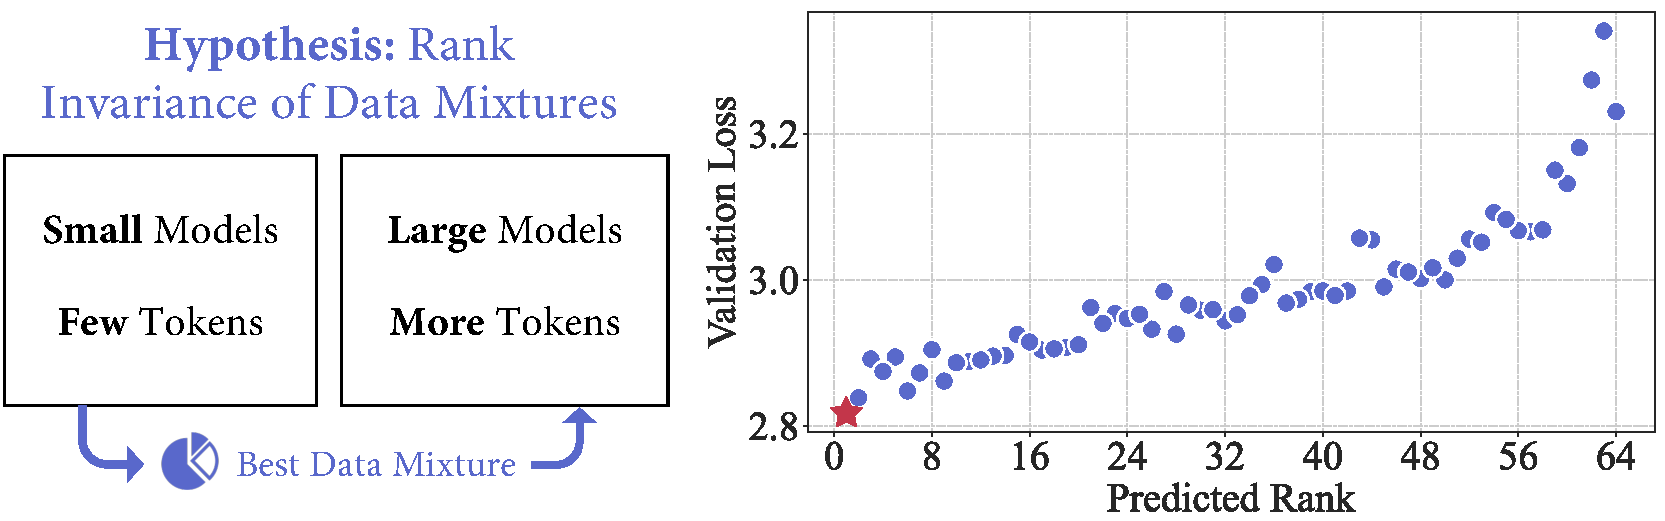
\includegraphics[width=1.0\textwidth]{figures/figure_1_overview.pdf}
    \caption{\textbf{Left}: We hypothesize the rank invariance of data mixtures across model sizes and numbers of training tokens. Leveraging this hypothesis, we use small models trained on fewer tokens to predict the effective data mixture for training large models with substantially more tokens. \textbf{Right}: By training $512 \times$ 1M models, our method identifies the best data mixture prior to training $64 \times$ 1B models. The predicted best data mixture, denoted by the red star, achieves the lowest validation loss.}
    \label{fig:1M_to_1B}
\end{figure}

The availability of large-scale public datasets has been a key factor enabling the creation of large language models (LLMs). Most data is available on the Internet and includes academic papers (e.g. arXiv), books (e.g. Project Gutenberg), and code (e.g. GitHub). For the creation of one of the first LLMs, GPT-3~\citep{gpt3paper}, the authors had already recognized the importance of selecting the best data for training, and thus they decided to upsample Wikipedia due to its perceived high quality. However, such manual data selection is not scalable and may lead to a suboptimal selection~\citep{albalak2024survey}.
As the size and diversity of data used for LLM pre-training continue to grow, determining the optimal data mixture becomes increasingly challenging.
It gives rise to the critical research question: \textit{How can we select the optimal data mixture in a scalable and efficient manner?} \looseness=-1

Prior work~\citep{xie2023doremi,fan2023doge,albalak2023efficient} employs small-scale models (``proxy models'') to predict the domain weights for large-scale language models. These works train proxy models with a substantial number of tokens (e.g., 100B), sometimes even the same number as used for training LLMs, and dynamically adjust the data allocation strategy by monitoring the training dynamics. However, these approaches become inefficient as the training data used for pre-training LLMs continues to grow.
Training a proxy model for current models, such as Llama-3, would require using up to 15T tokens~\citep{meta_llama_3_2024} with current approaches, which is likely too expensive and too slow to make it worthwhile~\footnote{These approaches often suffer from instability issues. Details can be found in Appendix~\ref{appendix:stability}.}.

In this work, we argue that \textit{training small models on a limited set of tokens} is sufficient to predict an effective data mixture for LLM training. Our key assumption is the \textit{rank invariance of data mixtures}, which posits that the relative ranking of data mixtures in terms of their impact on model performance is consistent across different model sizes and numbers of training tokens. Under this assumption, the key challenge lies in discovering the top-ranked data mixture from the near-infinite number of potential data mixtures. To do so, we treat the data mixture selection as a regression task. Rather than exhaustively training small models with every possible mixture, we train only a set of small models, each with a unique data mixture. Based on the performance of these models and their mixtures, we fit a regression model to predict the performance of other data mixtures. Our approach is significantly more scalable than prior work, as it allows for parallel training of small proxy models rather than training a single model for a long time. Further, the regression model provides insights into domain interactions that can facilitate understanding and data curation.  \looseness=-1

To validate \ourmethod, we train models with 1M and 1B parameters\footnote{Our model sizes mentioned in this paper refer to the number of non-embedding parameters, as embedding parameters account for a disproportionately large portion in smaller models.} with different data mixtures. By training 512 models with 1M parameters on 1B tokens\footnote{The estimated FLOPs for training $512 \times$ 1M models is nearly 2\% of the FLOPs required for one 1B model.}, we are able to predict the optimal data mixture among 64 models that are $1000 \times$ larger (1B parameters) and trained $25 \times$ longer (25B tokens) as depicted in Figure~\ref{fig:1M_to_1B}.
Moreover, the optimized data mixture using \ourmethod yields a better model than human selection, and achieves performance on par with the flagship DoReMi method~\citep{xie2023doremi} despite it requiring less total compute and allowing for parallel training.
We also find that (1) Data mixture significantly impacts downstream performance, resulting in substantial differences of up to 14.6\% in single-task performance; (2) General web corpora (e.g., CommonCrawl), rather than Wikipedia, exhibit the strongest positive correlation with improved performance across downstream tasks;
(3) The interactions between domains are complex and often contradict intuition, highlighting the need for automated approaches like \ourmethod. (4) Data mixture effects transcend scaling laws, and \ourmethod captures the complexity by considering all domains together. \looseness=-1

\section{Related work}

\textbf{Data selection and mixture} is concerned with curating data to optimize some goals, usually model performance~\citep{koh2017understanding,albalak2024survey}. Prior methods can be categorized into: \textbf{(1) Token-level} selection is the most fine-grained level of selection dealing with the filtering of tokens~\cite{lin2024rho1}.
\textbf{(2) Sample-level} selection is about choosing individual training examples. It is commonly employed for selecting fine-tuning data~\citep{thakkar2023self, das2023deft,xie2023data,engstrom2024dsdm,xia2024less, liu2023makes, bukharin2023data,kang2024get,mekala2024smaller, sachin2024selectllm,yang2024smalltolarge}. For the pre-training of LLMs, most methods rely on heuristics~\citep{rae2023gopher,sharma2024text,soldaini2024dolma}, but there have been some learned approaches using optimization algorithms~\citep{chen2024take,mindermann2022prioritized,shao2024balanced,yu2024mates}, model perplexity~\citep{marion2023investigating,muennighoff2023scaling}, or LLMs to inform the sample selection process~\citep{alex2024qurating,sachdeva2024train,zhang2024autonomous}. \textbf{(3) Group-level} selection assumes the data can be grouped into pools that are then optimally mixed. While early work again relies on manual mixtures~\citep{the_pile_corpus,gpt3paper}, learned mixtures have become more common~\citep{albalak2024survey}. Learned approaches either leverage proxy models to determine fixed weights for each group (``offline selection'')~\citep{rae2023gopher,xie2023doremi,fan2023doge} or dynamically adjust the weights during training of the final model (``online selection'')~\citep{chen2023skill}. Our approach, \ourmethod, is an offline group-level selection method. Different from the flagship algorithm in this category, DoReMi~\citep{xie2023doremi}, \ourmethod does not require training a single model for hundreds of thousands of steps, but instead a few small models for short durations. As these can be trained in parallel, our approach is more scalable, while also yielding better weights leading to a more performant final model.

\textbf{Data scaling laws} explore interactions of data quantity, quality, and mixing proportions, as LLMs are scaled up. \citet{muennighoff2023scaling} introduce scaling laws for data-constrained scenarios and \citet{goyal2024scaling} try to extend this approach to deal with multiple data pools. Prior research has confirmed that different datasets require different scaling~\citep{hoffmann2022training,pandey2024gzip}, thus \citet{ye2024datamixing} and \citet{ge2024data} propose functional relationships to predict the impact of mixtures on language modeling loss. Some work has investigated optimal mixtures during continued pre-training rather than from scratch training~\citep{que2024dcpt,dou2024sailor}. While most of these works focus on validation loss, others investigate downstream performance and develop predictive relations with loss~\citep{gadre2024language,yang2024fine,xia2022training}.
Different from data scaling work that attempt to find an analytical scaling function~\citep{hoffmann2022training}, \ourmethod directly optimizes the target metric using regression models.
\ourmethod is designed for from-scratch pre-training. In line with previous research, we also find strong correlations between loss and downstream performance, especially for loss on web corpora.

% While early works manually decide the mixture~\citep{the_pile_corpus}, later LLMs try to optimize mixture weights based on downstream performance~\citep{rae2023gopher}. DoReMi~\citep{xie2023doremi} shows that using a small proxy model trained for 200K steps, they can predict a data mixture of a 30x larger model that outperforms a human-selected mixture. Our method, \ourmethod, is a group-level selection algorithm.
% Additionally, some work finds that validation loss and downstream task performance. \citet{gadre2024language,yang2024fine} related language model perplexity to downstream metrics via a power law in the over-trained regime, while \citet{yang2024fine} compared model capabilities across pre-training checkpoints, confirming similar downstream metric dynamics across model sizes.
% Important for our work, because of our rank invariance assumption. These past works generally show that scaling behavior at small scale can be extrapolated to larger scales.
% Our work is different in that we do not require fitting a scaling law which can require lots of runs~\citep{hoffmann2022training} and we can choose any target metric.



% }
\section{\ourmethod: Data mixture as regression}

\begin{figure}[t]
    \vspace{-0.2cm}
    \centering
    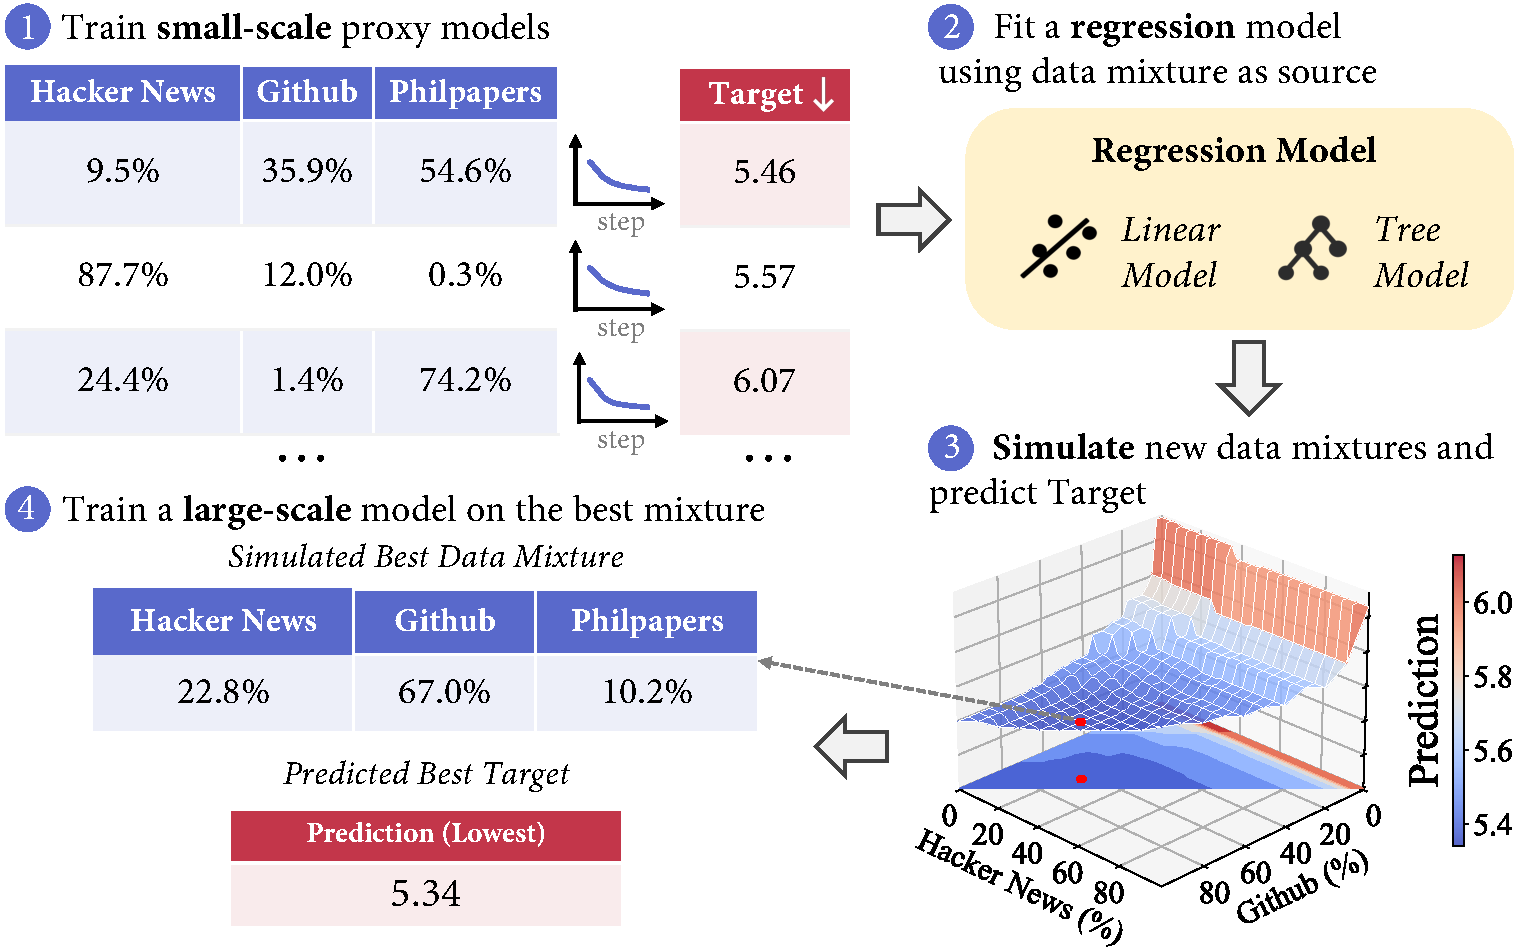
\includegraphics[width=0.9\textwidth]{figures/data_mixture_method_v9.pdf}
    \caption{The illustration of our method using Hacker News, GitHub, and Philpapers as training domains, with the loss on the StackExchange domain as the Target (where $\downarrow$ indicates lower is better). A regression model is fitted using small-scale proxy model training logs and employed to predict the best data mixture within the simulation space, enabling direct prediction of the data mixture for large-scale language model pre-training. Note that the Philpapers domain is omitted in the simulation plot (3) for simplicity.}
    \label{fig:method_overview}
    \vspace{-5mm}
\end{figure}

As illustrated in Figure~\ref{fig:method_overview}, our method involves four key steps: (1) Generate random data mixtures and train small-scale proxy models on these mixtures. (2) Fit a linear regression model using the mixtures as features and the target value as the label. (3) Simulate the data mixture space on a larger scale and leverage the regression model to identify the best mixture for the target value. (4) Train a large-scale model using the simulated best data mixture.

\subsection{Train small-scale proxy models}


The first step is to train a set of small-scale proxy models on multiple different data mixtures.
To reduce the required runs, we aim to select a diverse range of data mixtures that cover extreme weights from 0\% to 100\% for each domain.
We achieve this by using a Dirichlet distribution based on the token distribution, which allows us to sample a wide range of values and expose the regression models to various extremes.
Simultaneously, basing the distribution on the token distribution ensures that the overall data mixture statistically reflects the availability of data.
For example, this prevents any single domain with a token count below 1\% from being overly emphasized, which is not feasible for large-scale training since there are not enough available tokens from that domain.
In practice, we multiply the token distribution by a value from $0.1$ to $5.0$ to construct various sparse and near-uniform distributions, then use these distribution vectors as the Dirichlet distribution hyperparameter $\alpha$. \looseness=-1

After training small-scale proxy models for a few steps, we can obtain several well-trained small models. For example, in our main experiment, each proxy model contains 1M parameters and is trained on 1B tokens. We can then choose to evaluate these trained models on domains or benchmarks to get the target value we want to optimize.
Generally, the target value can be the loss on a domain, as shown in Figure~\ref{fig:method_overview} for the StackExchange domain.
Once we have obtained these target values, we can use the data mixture as features and the target values as labels to fit a regression model.

\subsection{Fit a regression model}

\begin{table*}[tb]
\centering
\small
\caption{Overview of the Pile dataset~\citep{the_pile_corpus} with datasets that are no longer available due to copyright issues marked in gray. In our experiments, we use the 17 available domains to study the data mixture for language model pre-training.}
\vspace{1mm}
\label{table:pile_overview}
\begin{tabular}{lr}
\toprule
\textbf{Component} & \textbf{Effective Size} \\
\midrule
Pile-CC  & 227.12 GiB  \\
PubMed Central & 180.55 GiB \\
\rowcolor{gray!25} Books3 & 151.44 GiB \\
\rowcolor{gray!25} OpenWebText2 & 125.54 GiB\\
ArXiv & 112.42 GiB \\
Github & 95.16 GiB\\
FreeLaw & 76.73 GiB \\
Stack Exchange & 64.39 GiB \\
USPTO Backgrounds & 45.81 GiB \\
PubMed Abstracts & 38.53 GiB \\
Gutenberg (PG-19) & 27.19 GiB \\
\bottomrule
\end{tabular}
\hspace{5mm}
\begin{tabular}{lr}
\toprule
\textbf{Component} & \textbf{Effective Size} \\
\midrule
\rowcolor{gray!25} OpenSubtitles & 19.47 GiB \\
Wikipedia (en) & 19.13 GiB \\
DM Mathematics  & 15.49 GiB \\
Ubuntu IRC & 11.03 GiB \\
\rowcolor{gray!25} BookCorpus2 & 9.45 GiB \\
EuroParl & 9.17 GiB \\
HackerNews & 7.80 GiB \\
\rowcolor{gray!25} YoutubeSubtitles & 7.47 GiB \\
PhilPapers & 4.76 GiB  \\
NIH ExPorter & 3.79 GiB  \\
Enron Emails & 1.76 GiB \\
\bottomrule
\end{tabular}
\vspace{-1mm}
\end{table*}

The second step is to fit a regression model using the data mixture as features, and the target value as labels.
The regression task is a conventional supervised learning task that involves predicting a continuous target variable $y$ based on input features $X = (x_1, x_2, \ldots, x_n)$. The goal is to find a function $f$ that best maps the input features to the target variable, such that $y=f(X) +\epsilon$, where $\epsilon$ represents the error or noise in the data. In the context of this paper, the input features $X$ correspond to the domain weights of the data mixture, and the target variable $y$ is the value we want to optimize. Using this data, we train regression models that learn a function to predict the target value based on arbitrary data mixtures without requiring further training.

\paragraph{Linear regression.}
The linear regression model is widely used in regression. It assumes a linear relationship between the input features and the target variable, which can be represented as:
\begin{equation}
y = \omega_0 + \omega_1 x_1 + \ldots + \omega_n x_n + \epsilon
\end{equation}
where $\omega_0$ is the intercept, and $\boldsymbol{\omega}=(\omega_1, \ldots, \omega_n)$ are the coefficients associated with the respective input features $x_1, \ldots, x_n$.
The coefficients $\boldsymbol{\omega}$ are typically estimated using techniques such as ordinary least squares, aiming to minimize the sum of squared residuals between the predicted and actual target values. In practice, we employ linear regression with L2 regularization, also known as ridge regression, which applies a penalty to the magnitude of $\boldsymbol{\omega}$ to prevent overfitting.

\paragraph{LightGBM regression.}
The LightGBM~\citep{ke2017lightgbm} is a powerful gradient-boosting algorithm that can be used for both regression and classification tasks. In the context of regression, LightGBM learns an ensemble of decision trees to predict the target variable. 
The process is guided by a gradient-based optimization algorithm, which minimizes a specified loss function (e.g. mean squared error). Moreover, LightGBM is designed to be efficient and scalable, making it suitable for large datasets.\looseness=-1

\subsection{Simulate and predict}

Once we have trained the regression model, we can efficiently explore the entire space of possible data mixtures.
By using the trained model to predict the target value for each potential data mixture, we can quickly identify the input that yields the best target value. This simulation-based optimization is relatively cheap, as both the simulation and the regression prediction are computationally fast. For example, running prediction for 1,000,000 data mixtures takes less than 10 CPU seconds.

\subsection{Large-scale model training}

After identifying the best data mixture with simulation, we generalize the top-ranked data mixture to a large-scale model training with many more tokens.  As shown in Figure~\ref{fig:method_overview}, we directly use the best data mixture for training the larger model. In practice, to increase the robustness of our regression prediction, we select the top $100$ mixtures and average them as the data mixture for large-scale training. \looseness=-1

\section{Evaluating on regression prediction}

\label{sec:evaluate_regression}

In this section, we evaluate the ability of \ourmethod to predict the effect of unseen data mixtures.
First, we fit the regression model using training artifacts of small (i.e., 1M parameter) models and evaluate the loss prediction performance on small models.
Then, to verify our \textit{rank invariance hypothesis}, we test the learned regression on predicting the rank across model sizes and the number of tokens.


\subsection{Experimental setup}

\paragraph{Datasets and models.}
We conduct our experiments using the domains of the Pile dataset~\citep{the_pile_corpus} depicted in Table~\ref{table:pile_overview}.
Due to copyright concerns, we utilize the 17 subsets available on HuggingFace~\footnote{\url{https://huggingface.co/datasets/monology/pile-uncopyrighted}} that do not violate copyright issues.
We consider both linear regression and LightGBM regression models, where the target variable $y$ is set to be the validation loss of the Pile-CC domain.


\begin{table}[t]
    \centering
    \small
    \caption{We fit the regression model based on the results of the $512 \times$ 1M models trained on 1B tokens, and evaluate it on \textbf{unseen data mixtures} for 1M, 60M, and 1B parameter models depicted below. Pearson's $r$ and MSE measure the loss prediction performance, while the Spearman correlation $\rho$ compares the predicted and actual ranks.}
    \label{tab:linear_vs_lightgbm}
    \scalebox{0.93}{
    \begin{tabular}{lccccccc}
        \toprule
        {Method} & \multicolumn{3}{c}{1M models with 1B tokens} & \multicolumn{2}{c}{60M models with 1B tokens} & \multicolumn{2}{c}{1B models with 25B tokens} \\
        \cmidrule(r){1-1} \cmidrule(lr){2-4} \cmidrule(lr){5-6} \cmidrule(lr){7-8}
         & \textbf{$\rho$ ($\uparrow$)} & {Pearson's $r$ ($\uparrow$)} &
         MSE ($\downarrow$) & $\rho$ ($\uparrow$) & {Pearson's $r$ ($\uparrow$)} & {$\rho$ ($\uparrow$)} & {Pearson's $r$ ($\uparrow$)} \\
        \midrule
        Linear & 90.08 & 87.78 & 0.13  & 89.26 & 86.79 & 88.01 & 72.57 \\
        LightGBM & \textbf{98.45} & \textbf{98.57} & \textbf{0.04} & \textbf{98.64} & \textbf{98.28} & \textbf{97.12} & \textbf{94.36} \\
        \bottomrule
    \end{tabular}
    }
    \vspace{1mm}
\end{table}

\paragraph{Training and evaluation.}
The regression model is fitted using the training artifacts of $512 \times$ 1M models with 1B tokens, and evaluated on $256 \times$ unseen data mixtures for 1M, 60M models (each trained with 1B tokens) and $64 \times$ unseen data mixtures for 1B models (each trained with 25B tokens).

\paragraph{Evaluation metrics.}
We use three different metrics to benchmark our regression models: (1) \textit{Spearman Rank Correlation ($\rho$)} is a non-parametric measure of the strength and direction of the association between two ranked variables. (2) \textit{Pearson's $r$} is a measure of the linear relationship between two variables. (3) \textit{Mean Squared Error (MSE)} is a common metric used to evaluate a regression model by measuring the average squared differences between predicted and actual values. 

\subsection{Experimental results}\label{sec:regression_results}


\paragraph{High correlation across model sizes.}
As shown in Table~\ref{tab:linear_vs_lightgbm}, the LightGBM model demonstrates superior performance over linear regression models across all three metrics, with its advantage becoming increasingly pronounced when evaluating on larger models with more training tokens.
Meanwhile, the fact that 1M models trained with 1B tokens can achieve such a high correlation of $97.12$\% on unseen mixtures of 1B models with 25B tokens directly validates our \textit{rank invariance hypothesis}. \looseness=-1


\paragraph{Proxy model count outweighs training token count.}
Given the same FLOPs budget for small-scale training, we can either increase the token count (i.e., the number of training tokens) or the number of proxy models. Therefore, we study which approach would yield better performance.
As shown in Figure~\ref{fig:1M-to-Test}, increasing the training tokens of the proxy models saturates after approximately 0.25B tokens.
In contrast, increasing the number of proxy models consistently enhances performance, particularly for the LightGBM model.
Notably, the performance of 512 models trained on 0.2B tokens surpasses that of 128 models trained on 0.8B tokens, indicating that increasing the number of proxy models is more effective than increasing the training token count beyond a certain token threshold. \looseness=-1
\section{Evaluating on downstream tasks}
\label{sec:app}


\begin{figure}[!t]
% \vspace{-0.8cm}
\vspace{-1mm}
\centering
\small
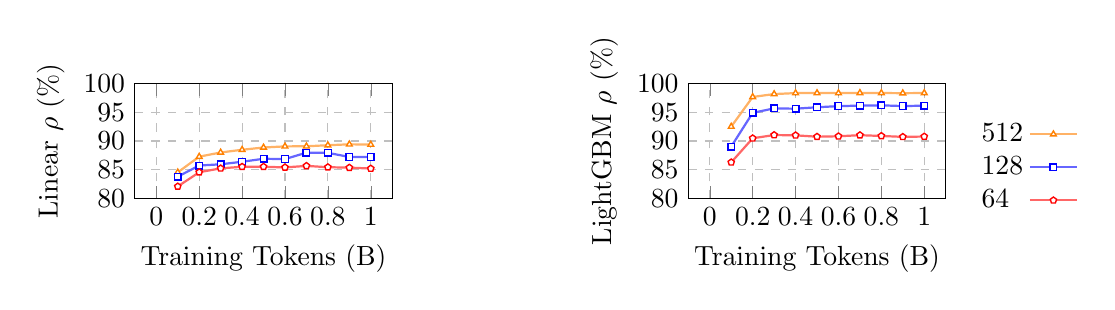
\begin{tikzpicture}
\begin{axis}[
at={(0em,0)},
width=.4\textwidth, height=.25\textwidth ,
xtick={0,0.2,...,1.0},
ytick={80, 85, ..., 105},
grid style=dashed,
ylabel={Linear $\rho$ (\%)},
xlabel={{Training Tokens (B)}},
xlabel style={align=center,yshift=0em},
ylabel style={yshift=0},
y tick style={opacity=0},
ymajorgrids=true,
xmajorgrids=true,
tick align=inside,
legend pos=outer north east,
yticklabel style={/pgf/number format/precision=0,/pgf/number format/fixed zerofill},
legend style={yshift=-0.5em,xshift=-9.7em,legend cell align=left,legend plot pos=right,draw=none},
xmin=-0.1,
xmax=1.1,
ymin=80.0,
ymax=100.0]

      \addplot[
        orange!60,mark=triangle*,mark size=1.2pt,thick,mark options={fill=white,draw=orange,line width=0.5pt}
        ]
        coordinates {
(0.1, 84.50739585717554)
(0.2, 87.25852597848477)
(0.3, 87.98917086289767)
(0.4, 88.46639677271683)
(0.5, 88.8603656443122)
(0.6, 89.05749313344012)
(0.7, 89.07301441977567)
(0.8, 89.2625600823987)
(0.9, 89.41834515907529)
(1.0, 89.3780041199359)
        };
      \addplot[
        blue!60,mark=square*,mark size=1.2pt,thick,mark options={fill=white,draw=blue,line width=0.5pt}
        ]
        coordinates {
(0.1, 83.76115815976193)
(0.2, 85.70146200503547)
(0.3, 85.92047665369648)
(0.4, 86.36615930418859)
(0.5, 86.88737411306934)
(0.6, 86.83294232089722)
(0.7, 87.96270599679559)
(0.8, 87.92558365758755)
(0.9, 87.2059538796063)
(1.0, 87.21818493934538)
        };
    \addplot[
        red!60,mark=pentagon*,mark size=1.2pt,thick,mark options={fill=white,draw=red,line width=0.5pt}
        ]
        coordinates {
(0.1, 82.03436140993362)
(0.2, 84.5289253833829)
(0.3, 85.20606832227053)
(0.4, 85.48960002288852)
(0.5, 85.48995765621422)
(0.6, 85.37587262531471)
(0.7, 85.63994907301439)
(0.8, 85.40898947127488)
(0.9, 85.33631837949186)
(1.0, 85.17452506294345)
        };
\end{axis}
\begin{axis}[
at={(20em,0)},
width=.4\textwidth, height=.25\textwidth ,
xtick={0,0.2,...,1.0},
ytick={80, 85, ..., 105},
grid style=dashed,
ylabel={LightGBM $\rho$ (\%)},
xlabel={{Training Tokens (B)}},
xlabel style={align=center,yshift=0em},
ylabel style={yshift=0},
y tick style={opacity=0},
ymajorgrids=true,
xmajorgrids=true,
tick align=inside,
legend pos=outer north east,
yticklabel style={/pgf/number format/precision=0,/pgf/number format/fixed zerofill},
legend style={yshift=-1.0em,xshift=0.5em,legend cell align=left,legend plot pos=right,draw=none},
xmin=-0.1,
xmax=1.1,
ymin=80,
ymax=100]
% \addplot[white!60,mark=triangle*,mark size=1.2pt,thick,mark options={fill=white,draw=white,line width=0.5pt}]coordinates {
% (0.0, 0.0)
% }; % dummy
      \addplot[
        orange!60,mark=triangle*,mark size=1.2pt,thick,mark options={fill=white,draw=orange,line width=0.5pt}
        ]
        coordinates {
(0.1, 92.5231746395056)
(0.2, 97.71550984206911)
(0.3, 98.22535191119248)
(0.4, 98.39100766765847)
(0.5, 98.39830338750286)
(0.6, 98.39050698100249)
(0.7, 98.42104886701762)
(0.8, 98.40695811398487)
(0.9, 98.37613012130923)
(1.0, 98.40960460059507)
        };
      \addplot[
        blue!60,mark=square*,mark size=1.2pt,thick,mark options={fill=white,draw=blue,line width=0.5pt}
        ]
        coordinates {
(0.1, 89.02838178072784)
(0.2, 94.935983634699)
(0.3, 95.712405584802)
(0.4, 95.66004806591896)
(0.5, 95.91268024719614)
(0.6, 96.11080910963605)
(0.7, 96.19771400778208)
(0.8, 96.24749656672006)
(0.9, 96.1234865178486)
(1.0, 96.18727111467155)
        };
    \addplot[
        red!60,mark=pentagon*,mark size=1.2pt,thick,mark options={fill=white,draw=red,line width=0.5pt}
        ]
        coordinates {
(0.1, 86.26339159912636)
(0.2, 90.47847422125)
(0.3, 91.04610683661835)
(0.4, 90.99587559002012)
(0.5, 90.75215395088516)
(0.6, 90.82915943331062)
(0.7, 91.02118619821466)
(0.8, 90.88363390053959)
(0.9, 90.72496478655565)
(1.0, 90.78300240329592)
        };
        % \legend{{Title}, {512},{128},{64}}
        \legend{{512},{128},{64}}
\end{axis}
\end{tikzpicture}
\vspace{-2mm}
\caption{The plot of Spearman Rank Correlation $\rho$ between the predicted ranks and true ranks of Linear regression (\textbf{Left}) and LightGBM regression (\textbf{Right}) across different training tokens and different number of proxy models. As shown, increasing the number of proxy models significantly boosts $\rho$, while adding more training tokens has diminishing returns. 
% \niklas{Are the `.00` on the y-axis necessary here? I think we can remove them}
}
\label{fig:1M-to-Test}
% \vspace{-2mm}
\end{figure}



In this section, we apply our method to demonstrate its effectiveness on realistic downstream tasks. For evaluation, we exclude specific benchmarks that exhibit large performance variance (e.g., RTE) according to the performance traces reported in previous work~\citep{openelm2024} and our observations during pre-training.
Ultimately, we select the following benchmarks as our downstream tasks: Social IQA~\citep{sap2019socialiqa}, HellaSwag~\citep{zellers2019hellaswag}, PiQA~\citep{bisk2020piqa}, OpenBookQA~\citep{mihaylov2018can}, Lambada~\citep{paperno2016lambada}, SciQ~\citep{welbl2017crowdsourcing}, ARC Easy~\citep{clark2018think}, COPA~\citep{sarlin2020superglue}, RACE~\citep{lai2017race}, LogiQA~\citep{liu2020logiqa}, QQP~\citep{wang2018glue}, WinoGrande~\citep{sakaguchi2021winogrande}, and MultiRC~\citep{khashabi2018looking}. These benchmarks cover a diverse range of tasks, enabling a comprehensive evaluation of the real-world impact of \ourmethod. For each benchmark, we use normalized accuracy as the evaluation metric if provided by lm-eval-harness~\citep{eval-harness} else we use regular accuracy.


\subsection{Data mixture significantly impacts downstream performance}

\begin{table}[t]
    \centering
    \small
    \caption{We experiment with 64 models, each with 1B parameters trained on different data mixtures, and evaluate their performance across various benchmarks. The reported performance on each task is the average score from 0-shot to 5-shot settings, following~\citet{muennighoff2023scaling}. Here, we present the worst and best model performances on each task, and detailed experimental results for individual models can be found in Appendix~\ref{appendix:all_model_results}.}
    \label{tab:worst_best_model_perf}
    \begin{tabular}{l|ccc}
    \toprule
     \textbf{Benchmark} & \textbf{Worst Model} & \textbf{Best Model} & $\Delta$ \\
     \midrule
        Social IQA~\citep{sap2019socialiqa} & 32.4 & 33.9 & 1.5 \\
        HellaSwag~\citep{zellers2019hellaswag} & 33.0 & 43.4 & 10.4 \\
        PiQA~\citep{bisk2020piqa} & 60.2 & 69.0 & 8.8 \\
        OpenBookQA~\citep{mihaylov2018can} & 25.8 & 31.2 & 5.4 \\
        Lambada~\citep{paperno2016lambada} & 18.9 & 33.5 & 14.6 \\
        SciQ~\citep{welbl2017crowdsourcing} & 76.7 & 82.9 & 6.2 \\
        ARC Easy~\citep{clark2018think} & 44.9 & 52.2 & 7.3 \\
        COPA~\citep{sarlin2020superglue}  & 61.5 & 70.5 & 9.0 \\
        RACE~\citep{lai2017race}  & 27.9 & 32.5 & 4.6 \\
        LogiQA~\citep{liu2020logiqa}  & 23.2 & 27.7 & 4.5 \\
        QQP~\citep{wang2018glue}  & 48.0 & 59.7 & 11.7 \\
        WinoGrande~\citep{sakaguchi2021winogrande} & 50.3 & 53.2 & 2.9 \\
        MultiRC~\citep{khashabi2018looking} & 47.6 & 55.7 & 8.1 \\
        \midrule
        Average Performance & 43.7 & 47.9 & 4.2 \\
    \bottomrule
    \end{tabular}
\end{table}

Initially, we train 64 models, each with 1B parameters, using different data mixtures.
Every model is trained on 25B tokens\footnote{We set the token quantity such that it is compute-optimal according to the Chinchilla scaling law~\citep{hoffmann2022training}.} from the Pile dataset~\citep{the_pile_corpus}, with tokens allocated based on their corresponding domain weights.
Table~\ref{tab:worst_best_model_perf} presents the performance of the worst and best models on each downstream task. The reported performance is the average from 0-shot to 5-shot evaluations, scored using the lm-eval-harness evaluation framework~\citep{eval-harness,biderman2024lessons}. We find that the data mixture significantly impacts downstream performances, with the largest performance $\Delta$ reaching $14.6$ on the Lambada task. This underscores the importance of studying the optimal data mixture.

\subsection{Web corpora benefits downstream performance the most}

\begin{figure}[t]
    \centering
    \subfigure[Correlation between validation loss by domains of the Pile and downstream performance.]{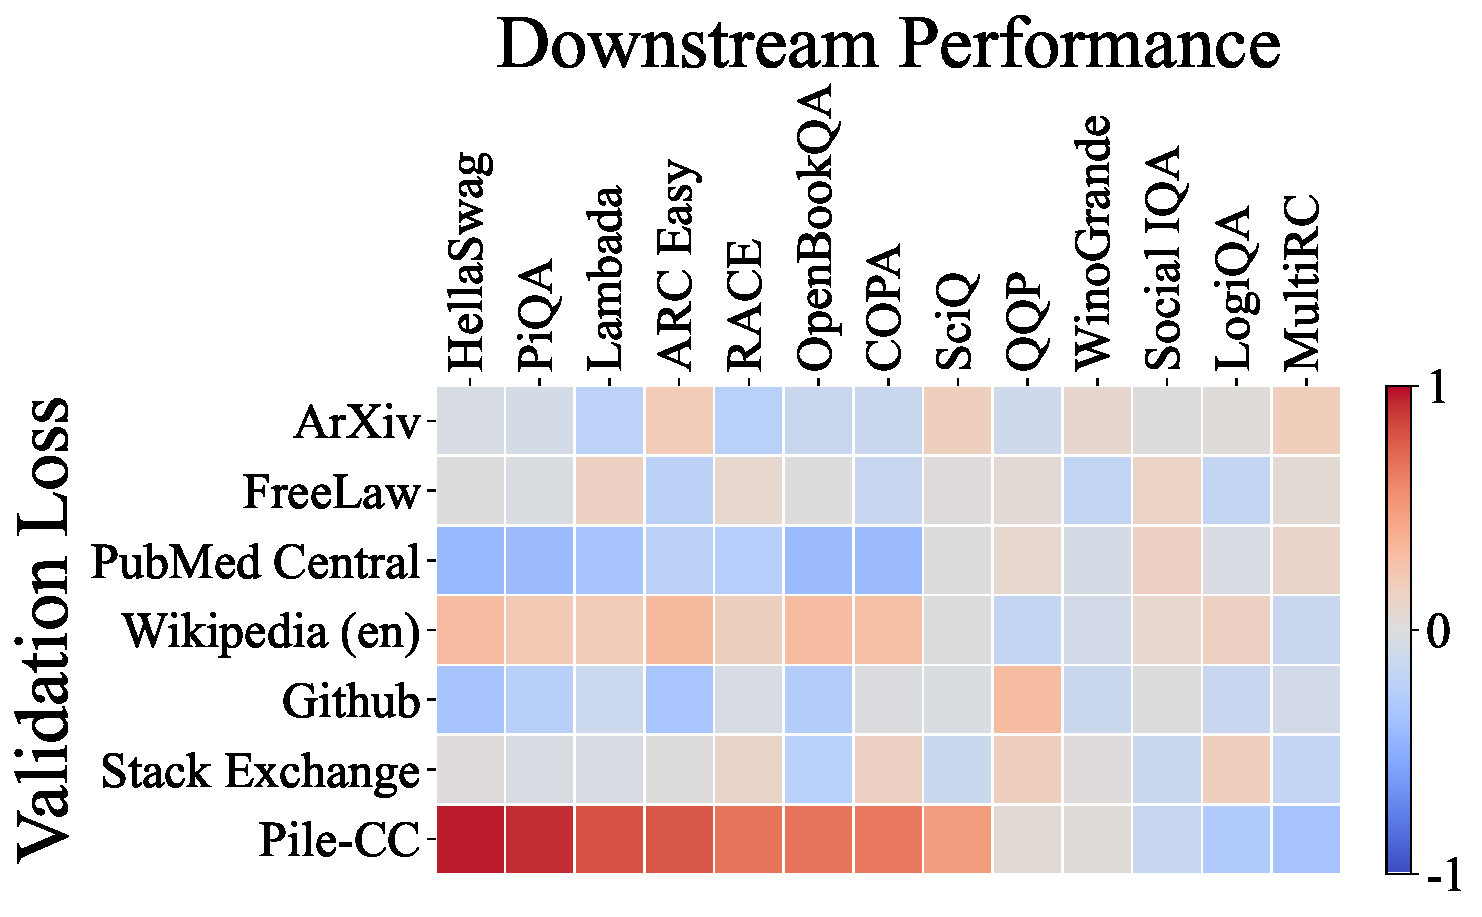
\includegraphics[height=0.28\textwidth]{figures/Domain_and_Task.pdf}}
    \hspace{1mm}
    \subfigure[Correlation between validation loss by URL domain within the Pile-CC subset and downstream performance.]
    {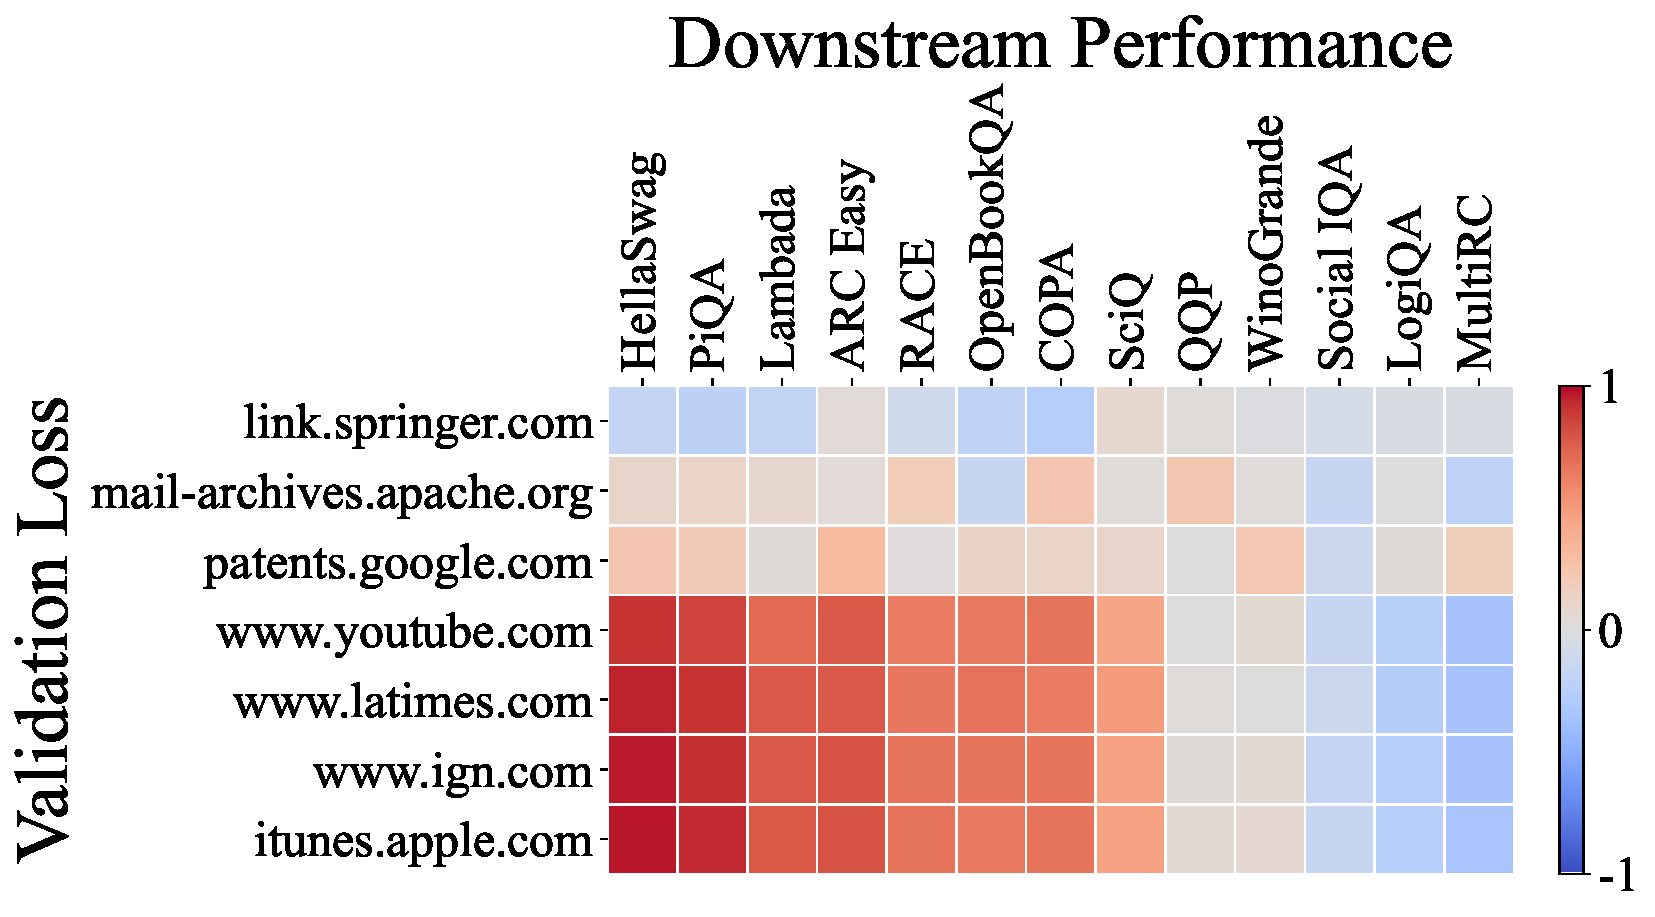
\includegraphics[height=0.28\textwidth]{figures/Domain_and_Task_c4100.pdf}}
    \caption{The correlation between validation losses across domains and downstream performance for the $64 \times$ 1B models. Note that we take the negative of the loss value when calculating the correlation, as this makes the visualization more intuitive. The same applies for Figure~\ref{fig:domain_interaction}. }
    \label{fig:domain-and-task}
\end{figure}

Next, we visualize the correlation between the validation losses of our 64 1B models across different domains and their performance on various downstream tasks in Figure~\ref{fig:domain-and-task} (a). Prior to visualization, we hypothesized that the validation loss on the Wikipedia (en) subset would exhibit a strong correlation with most downstream tasks, as it is a high-quality dataset, and many downstream tasks are derived from Wikipedia text. Similarly, previous work often takes WikiText~\citep{merity2016pointer} as a standard benchmark to indicate language model performance.

However, surprisingly, the validation loss on the Pile-CC dataset shows the strongest correlation with most downstream tasks. For instance, the correlation coefficient between the HellaSwag task and the Pile-CC validation loss is remarkably close to $1.0$.
This unexpected result challenges the conventional assumption that WikiText is the most representative dataset for evaluating LLMs.
Furthermore, this result aligns with the findings of previous studies~\citep{gadre2024language, huang2024compression}, which discovered that the validation loss on the web dataset closely relates to downstream performance. 

Moreover, we analyze the correlation between the loss of models on the C4100Domain validation set~\citep{paloma2023allen}, which is taken from the C4 dataset~\citep{2019t5} and supposed to share a similar distribution as Pile-CC since they are all derived from the CommonCrawl corpus. Since CommonCrawl is a collection of diverse domains, we would expect the correlation between the loss of each domain and the downstream tasks to vary. However, surprisingly more than 85\% of the domains exhibit a very strong correlation with Pile-CC (full correlation graph in Appendix~\ref{appendix:correaltion_graph}).
This is exemplified by the \texttt{www.ign.com} domain, which closely mirrors the overall correlation graph of Pile-CC, as illustrated in Figure~\ref{fig:domain-and-task} (b).
It also suggests that the high correlation between Pile-CC and downstream task performance may be attributed to its \textit{diverse coverage across various topics and domains}.

\subsection{Data mixture by \ourmethod improves downstream performance}
\label{sec:no_pile_exper}


\begin{table}[tb]
    \centering
    \small
    \caption{Performance comparison of different data selection methods. Human refers to the weights put forth in The Pile~\citep{the_pile_corpus}, Pile-CC Only to only training on the Pile-CC component, and DoReMi to the weights from \citet{xie2023doremi}. The reported performance for each task is the average score across 0-shot to 5-shot settings across five different runs, and the standard deviation. We estimate the compute (measured in FLOPs) required to arrive at the training data mixture. Scores significantly outperforming the Human baseline for each task are highlighted in \textbf{bold}, with significance determined using Cohen's d. To provide a comprehensive assessment, we also report the evaluation results using LightEval, following the setup by \citet{penedo2024finewebdatasetsdecantingweb} in Appendix~\ref{appendix:lighteval}. The LightEval results indicate that \ourmethod performs slightly better than DoReMi and Pile-CC Only.}
    \label{tab:downstream_perf_our}
    \begin{tabular}{l|l|lll}
    \toprule
         \textbf{Benchmark} & \textbf{Human} & \textbf{DoReMi} & \textbf{Pile-CC Only} & \textbf{\ourmethod} \\
    \midrule
        Social IQA~\citep{sap2019socialiqa} & {33.8}\text{\,\scriptsize$\pm$\,0.4} &  33.3\text{\,\scriptsize$\pm$\,\,0.2} &  33.4\text{\,\scriptsize$\pm$\,0.4} &  33.5\text{\,\scriptsize$\pm$\,0.2}  \\ 
        HellaSwag~\citep{zellers2019hellaswag} & 37.7\text{\,\scriptsize$\pm$\,0.2} & \textbf{43.3}\text{\,\scriptsize$\pm$\,0.3} & \textbf{43.2}\text{\,\scriptsize$\pm$\,0.6} & \textbf{44.0}\text{\,\scriptsize$\pm$\,0.2}  \\ 
        PiQA~\citep{bisk2020piqa} &  65.5\text{\,\scriptsize$\pm$\,0.7} & \textbf{68.6}\text{\,\scriptsize$\pm$\,0.4} & \textbf{68.8}\text{\,\scriptsize$\pm$\,0.6} & \textbf{69.1}\text{\,\scriptsize$\pm$\,0.4}  \\ 
        OpenBookQA~\citep{mihaylov2018can} & {28.5}\text{\,\scriptsize$\pm$\,0.4} & \textbf{30.0}\text{\,\scriptsize$\pm$\,0.3} & \textbf{30.5}\text{\,\scriptsize$\pm$\,0.4} & \textbf{29.8}\text{\,\scriptsize$\pm$\,0.5}  \\ 
        Lambada~\citep{paperno2016lambada} & {28.3}\text{\,\scriptsize$\pm$\,1.5}& \textbf{32.4}\text{\,\scriptsize$\pm$\,0.7} & \textbf{34.2}\text{\,\scriptsize$\pm$\,1.1} & \textbf{32.9}\text{\,\scriptsize$\pm$\,1.4}  \\
        SciQ~\citep{welbl2017crowdsourcing} & {81.5}\text{\,\scriptsize$\pm$\,1.1} & {\textbf{83.3}}\text{\,\scriptsize$\pm$\,1.9} & {82.4}\text{\,\scriptsize$\pm$\,1.0} & \textbf{82.8}\text{\,\scriptsize$\pm$\,0.4} \\ 
        ARC Easy~\citep{clark2018think} & 49.9\text{\,\scriptsize$\pm$\,0.9} &  {\textbf{52.3}}\text{\,\scriptsize$\pm$\,1.1} &  \textbf{51.8}\text{\,\scriptsize$\pm$\,0.4} & \textbf{52.1}\text{\,\scriptsize$\pm$\,0.9}  \\ 
        COPA~\citep{sarlin2020superglue} & 64.6\text{\,\scriptsize$\pm$\,1.8} & \textbf{69.7}\text{\,\scriptsize$\pm$\,2.7} & \textbf{67.5}\text{\,\scriptsize$\pm$\,2.0} & {\textbf{69.9}}\text{\,\scriptsize$\pm$\,0.6}  \\ 
        RACE~\citep{lai2017race} & {29.5}\text{\,\scriptsize$\pm$\,0.5} & \textbf{31.1}\text{\,\scriptsize$\pm$\,0.2} & {\textbf{31.5}}\text{\,\scriptsize$\pm$\,0.5} & \textbf{31.2}\text{\,\scriptsize$\pm$\,0.4} \\ 
        LogiQA~\citep{liu2020logiqa} & 25.7\text{\,\scriptsize$\pm$\,0.8} & 25.5\text{\,\scriptsize$\pm$\,0.7}& {26.6}\text{\,\scriptsize$\pm$\,1.0} & 25.4\text{\,\scriptsize$\pm$\,1.2} \\ 
        QQP~\citep{wang2018glue} & 55.6\text{\,\scriptsize$\pm$\,2.9} & 57.3\text{\,\scriptsize$\pm$\,1.4} & {\textbf{58.0}}\text{\,\scriptsize$\pm$\,1.9} &  55.7\text{\,\scriptsize$\pm$\,1.9}  \\ 
        WinoGrande~\citep{sakaguchi2021winogrande} & 52.0\text{\,\scriptsize$\pm$\,1.0}  & {52.1}\text{\,\scriptsize$\pm$\,0.3}  & 51.8\text{\,\scriptsize$\pm$\,0.7}  & {52.1}\text{\,\scriptsize$\pm$\,0.7}   \\ 
        MultiRC~\citep{khashabi2018looking} & {52.9}\text{\,\scriptsize$\pm$\,1.4} & {52.9}\text{\,\scriptsize$\pm$\,1.2} &  {51.2}\text{\,\scriptsize$\pm$\,1.5} &  {52.8}\text{\,\scriptsize$\pm$\,1.5} \\
        \midrule
        Average Performance & 46.6\text{\,\scriptsize$\pm$\,0.3} & 48.6\text{\,\scriptsize$\pm$\,0.3} & 48.5\text{\,\scriptsize$\pm$\,0.3} & 48.6\text{\,\scriptsize$\pm$\,0.3} \\
        Beat Human on & -- & 8 / 13 & 8 / 13 & 8 / 13 \\
        Estimated FLOPs & 0 & $3.7\times10^{19}$ & 0 & $3.5\times10^{18}$ \\
    \bottomrule
    \end{tabular}
\end{table}

Previous work has shown that the data mixture method can accelerate LLM pre-training by achieving a smaller validation loss (or perplexity) using less training tokens~\citep{xie2023doremi}. However, a key question is \textit{which validation loss should be optimized?}
The most intuitive approach, which is also adopted by previous work, is to minimize the loss across all domains. However, based on our study of 1M training logs, we found this to be nearly impossible to achieve in practice. None of the data mixtures were able to surpass the human selection on all domain validation losses simultaneously. This suggests that a naive approach of minimizing the loss across all domains is likely infeasible. Therefore, we choose to optimize the Pile-CC validation loss to achieve general performance improvement on downstream tasks since it shows the highest correlation with downstream performance.

We implement two approaches to determine the data mixture.
The first approach relies on human intuition.
Since Pile-CC and its own distribution should be the closest match, we hypothesized that pre-training solely on Pile-CC might yield better performance than baselines.
The second approach leverages \ourmethod, using the Pile-CC validation loss as the target variable. We employed LightGBM to predict the data mixture which can minimize the Pile-CC validation loss. \looseness=-1

We compare the performance of our proposed approaches to strong baselines, including selection done by humans for the Pile~\citep{the_pile_corpus}, and DoReMi~\citep{xie2023doremi}. For DoReMi we obtain the data mixture directly from their reported best domain weights and re-normalize it across the available 17 domains. This may result in sub-optimal performance for DoReMi compared to the originally reported results. As shown in Table~\ref{tab:downstream_perf_our}, both Pile-CC Only and \ourmethod demonstrate strong performance compared to the baselines. On the widely used HellaSwag benchmark, \ourmethod shows an improvement of $6.8$ over Human selection. Additionally, \ourmethod beats all other three methods on the task performance in 8 out of 14 cases and yields the highest average score. The surprisingly strong performance of Pile-CC Only reinforces the conclusion from our previous section: web corpora benefits on downstream performance. Finally, \ourmethod surpasses the Best Model in Table~\ref{tab:worst_best_model_perf}, demonstrating that our automatic data mixture approach is more efficient than random search.


\begin{figure}[!t]
% \vspace{-0.8cm}
\centering
\small
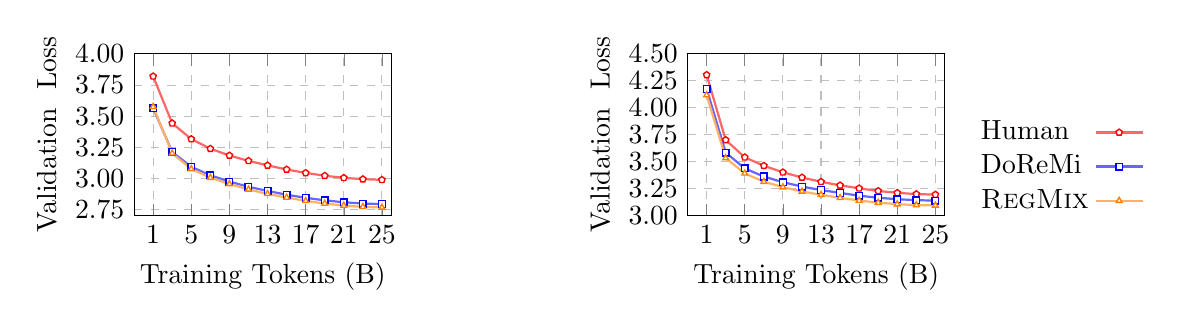
\begin{tikzpicture}
\begin{axis}[
at={(0em,0)},
width=.4\textwidth, height=.3\textwidth ,
xtick={1,5,...,25},
ytick={2.75, 3.0, ..., 4.5},
grid style=dashed,
ylabel={Validation\ \ Loss},
xlabel={{Training Tokens (B)}},
xlabel style={align=center,yshift=0em},
ylabel style={yshift=0},
y tick style={opacity=0},
ymajorgrids=true,
xmajorgrids=true,
tick align=inside,
legend pos=outer north east,
yticklabel style={/pgf/number format/precision=2,/pgf/number format/fixed zerofill},
legend style={yshift=-0.5em,xshift=-9.7em,legend cell align=left,legend plot pos=right,draw=none},
xmin=-1,
xmax=26,
ymin=2.7,
ymax=4.0]
    \addplot[
        red!60,mark=pentagon*,mark size=1.2pt,thick,mark options={fill=white,draw=red,line width=0.5pt}
        ]
        coordinates {
(1, 3.820050001)
% (2, 3.563014746)
(3, 3.443202972)
% (4, 3.371057034)
(5, 3.316340208)
% (6, 3.273290396)
(7, 3.238892794)
% (8, 3.210097551)
(9, 3.184519053)
% (10, 3.161157131)
(11, 3.141363859)
% (12, 3.121436596)
(13, 3.104880571)
% (14, 3.088854313)
(15, 3.072213173)
% (16, 3.058333397)
(17, 3.04462266)
% (18, 3.032625914)
(19, 3.021899939)
% (20, 3.012994051)
(21, 3.00503087)
% (22, 2.999095917)
(23, 2.994301796)
% (24, 2.991042376)
(25, 2.989006996)
        };
      \addplot[
        blue!60,mark=square*,mark size=1.2pt,thick,mark options={fill=white,draw=blue,line width=0.5pt}
        ]
        coordinates {
(1, 3.564236641)
% (2, 3.318056822)
(3, 3.212352514)
% (4, 3.141084194)
(5, 3.092962027)
% (6, 3.051904917)
(7, 3.025346518)
% (8, 2.99630475)
(9, 2.975091696)
% (10, 2.951140165)
(11, 2.93320632)
% (12, 2.914949179)
(13, 2.89994359)
% (14, 2.884443521)
(15, 2.869195461)
% (16, 2.857667685)
(17, 2.844691038)
% (18, 2.833688259)
(19, 2.824284554)
% (20, 2.815539598)
(21, 2.808733463)
% (22, 2.803073645)
(23, 2.798743486)
% (24, 2.795792103)
(25, 2.793961763)
        };
      \addplot[
        orange!60,mark=triangle*,mark size=1.2pt,thick,mark options={fill=white,draw=orange,line width=0.5pt}
        ]
        coordinates {
(1, 3.575109243)
% (2, 3.322744131)
(3, 3.201750994)
% (4, 3.126943827)
(5, 3.07610321)
% (6, 3.03995347)
(7, 3.006507158)
% (8, 2.976192474)
(9, 2.955598593)
% (10, 2.932467222)
(11, 2.911984682)
% (12, 2.894156218)
(13, 2.876117468)
% (14, 2.859216928)
(15, 2.846674204)
% (16, 2.832516909)
(17, 2.820066452)
% (18, 2.809194803)
(19, 2.798643112)
% (20, 2.789196491)
(21, 2.782349825)
% (22, 2.776001453)
(23, 2.771711111)
% (24, 2.76859498)
(25, 2.76705265)
        };
        % \legend{\tiny{Human},\tiny{DoreMi},\tiny{\ourmethod}}
\end{axis}
\begin{axis}[
at={(20em,0)},
width=.4\textwidth, height=.3\textwidth ,
xtick={1,5,...,25},
ytick={2.75, 3.0, ..., 4.5},
grid style=dashed,
ylabel={Validation\ \ Loss},
xlabel={{Training Tokens (B)}},
xlabel style={align=center,yshift=0em},
ylabel style={yshift=0},
y tick style={opacity=0},
ymajorgrids=true,
xmajorgrids=true,
tick align=inside,
legend pos=outer north east,
yticklabel style={/pgf/number format/precision=2,/pgf/number format/fixed zerofill},
legend style={yshift=-2em,xshift=0.5em,legend cell align=left,legend plot pos=right,draw=none},
xmin=-1,
xmax=26,
ymin=3.0,
ymax=4.50]
    \addplot[
        red!60,mark=pentagon*,mark size=1.2pt,thick,mark options={fill=white,draw=red,line width=0.5pt}
        ]
        coordinates {
(1, 4.305472374)
% (2, 3.856157064)
(3, 3.702566862)
% (4, 3.607195139)
(5, 3.542406321)
% (6, 3.499405861)
(7, 3.463979483)
% (8, 3.427306652)
(9, 3.402868032)
% (10, 3.375495434)
(11, 3.355190039)
% (12, 3.334785461)
(13, 3.315196753)
% (14, 3.296992064)
(15, 3.28206563)
% (16, 3.267296791)
(17, 3.254812002)
% (18, 3.240809202)
(19, 3.230043173)
% (20, 3.220910549)
(21, 3.213106632)
% (22, 3.206263304)
(23, 3.201158285)
% (24, 3.197825193)
(25, 3.196551085)
        };
      \addplot[
        blue!60,mark=square*,mark size=1.2pt,thick,mark options={fill=white,draw=blue,line width=0.5pt}
        ]
        coordinates {
(1, 4.17596674)
% (2, 3.736148596)
(3, 3.586002111)
% (4, 3.499732018)
(5, 3.438609838)
% (6, 3.398218393)
(7, 3.364253044)
% (8, 3.333914757)
(9, 3.311367512)
% (10, 3.291027069)
(11, 3.271058083)
% (12, 3.253663778)
(13, 3.238744497)
% (14, 3.22495842)
(15, 3.212095261)
% (16, 3.199076176)
(17, 3.186464071)
% (18, 3.176945448)
(19, 3.167378426)
% (20, 3.159505844)
(21, 3.153804779)
% (22, 3.148664713)
(23, 3.14490509)
% (24, 3.142236948)
(25, 3.140860558)
        };
      \addplot[
        orange!60,mark=triangle*,mark size=1.2pt,thick,mark options={fill=white,draw=orange,line width=0.5pt}
        ]
        coordinates {
(1, 4.119034767)
% (2, 3.685588598)
(3, 3.535004854)
% (4, 3.449685335)
(5, 3.393175602)
% (6, 3.349918127)
(7, 3.316093445)
% (8, 3.289763212)
(9, 3.265641689)
% (10, 3.245405912)
(11, 3.225485563)
% (12, 3.210350275)
(13, 3.195032358)
% (14, 3.17729187)
(15, 3.166511536)
% (16, 3.15453434)
(17, 3.141429901)
% (18, 3.133812904)
(19, 3.121953964)
% (20, 3.114748478)
(21, 3.107906342)
% (22, 3.103094816)
(23, 3.099808216)
% (24, 3.097485781)
(25, 3.095982313)
        };
        \legend{{Human},{DoReMi},{\ourmethod}}
\end{axis}
\end{tikzpicture}
\vspace{-5mm}
\caption{\textbf{Left}: The validation loss on Pile-CC of different methods with Pile-CC in the pre-training corpus. \textbf{Right}: The validation loss on Pile-CC excluding Pile-CC in the pre-training.}
\label{fig:loss_curve}
\vspace{-1mm}
\end{figure}



While the Pile-CC validation loss is an informative indicator for downstream performance, it may not generalize to every task of interest. Sometimes we may not be able to assume that the validation set stems from a similar data distribution as the training set, but rather face an out-of-distribution scenario.
To verify the effectiveness of our method in out-of-distribution scenarios, we fully exclude the Pile-CC domain from the pre-training corpus and use the remaining domains to find the optimal data mixture that minimizes Pile-CC validation loss. As illustrated in Figure~\ref{fig:loss_curve} (right), our proposed method still outperforms baseline approaches. This demonstrates that \ourmethod is robust regardless of whether the target domain is in- or out-of-distribution.
We additionally provide the results of regression evaluation under this setting in Figure~\ref{tab:linear_vs_lightgbm_1M_OOD}.

\subsection{Domain interactions are challenging for humans to understand}\label{sec:domain_interaction}


\begin{figure}[t]
    \centering
    \subfigure{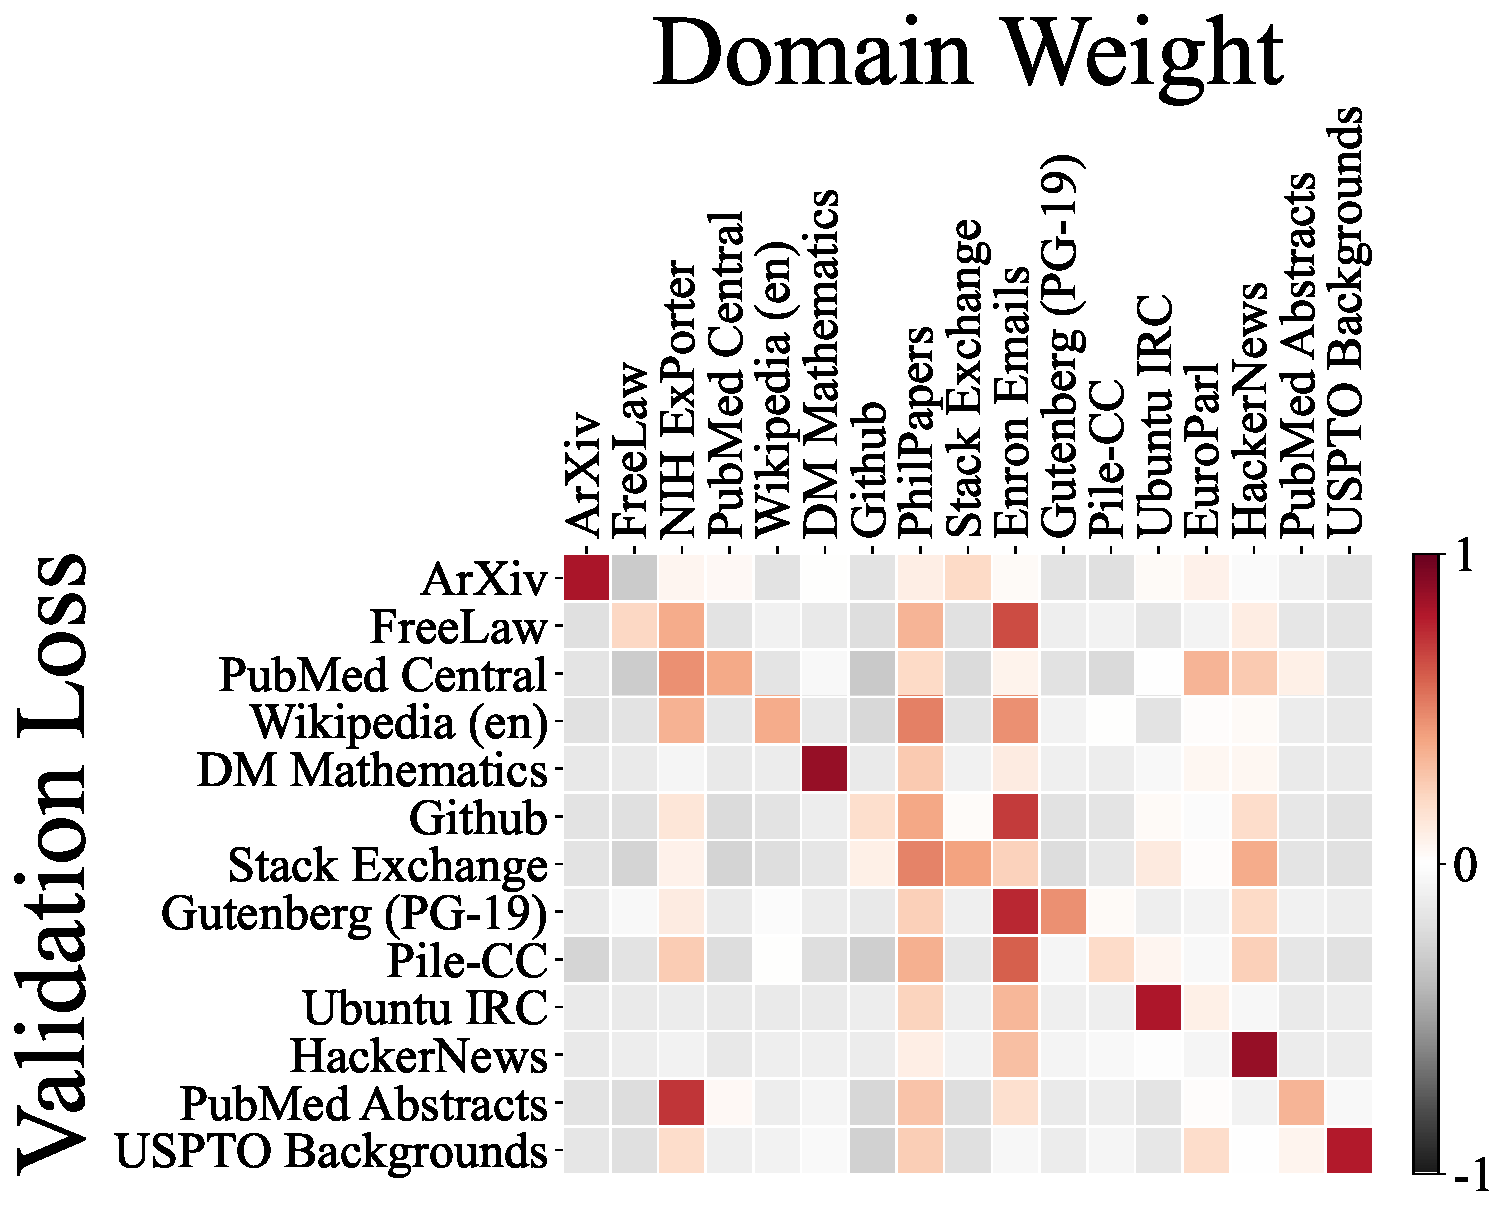
\includegraphics[height=.285\textwidth]{figures/1M_pile_4B_w.pdf}}
    \subfigure{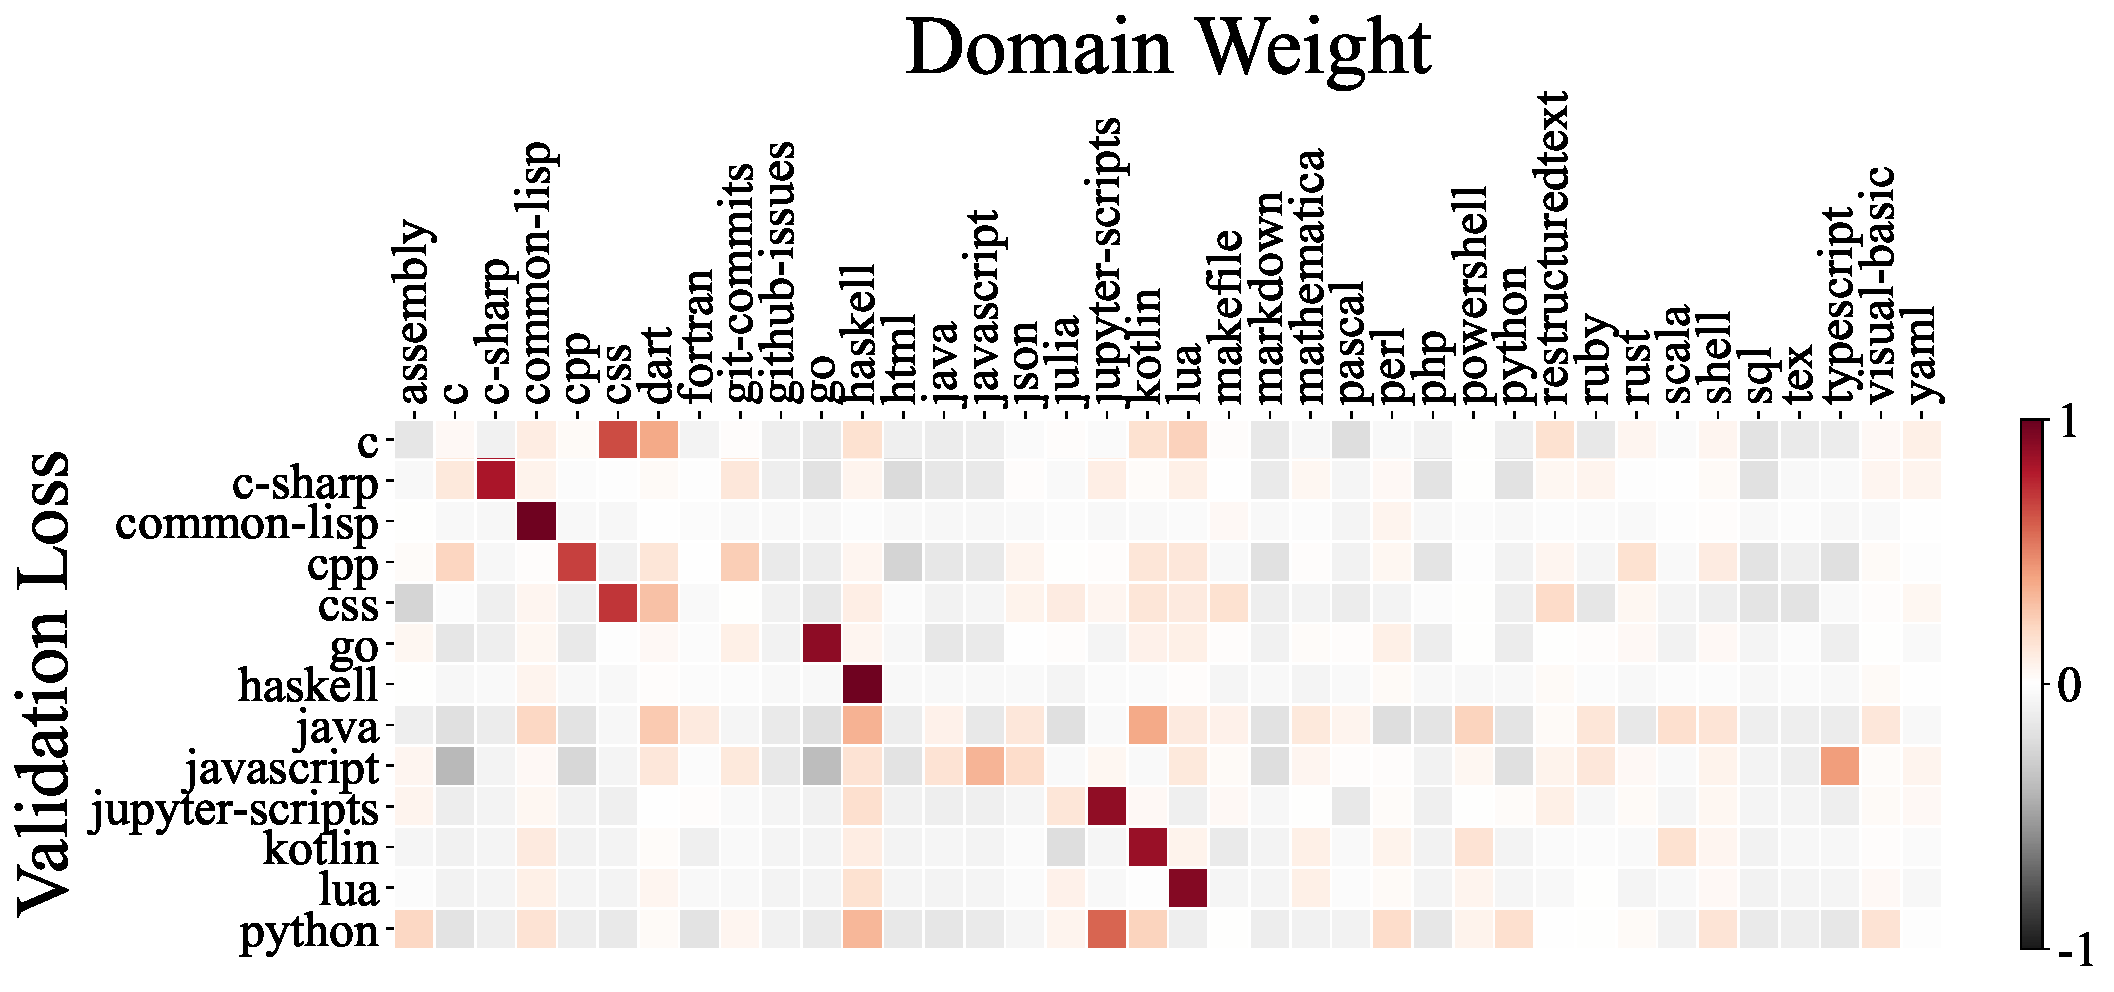
\includegraphics[height=.285\textwidth]{figures/1M_code_w.pdf}}
    \caption{The visualization of correlations between different target domain validation losses and training domain weights using the linear regression model. \textbf{Left} is on the Pile dataset, and \textbf{Right} is on the Stack dataset. A high correlation indicates that increasing the training domain weight has a positive impact on reducing the target domain validation loss. }
    \label{fig:domain_interaction}
\end{figure}

To understand the impact of different domains on each other, we visualize the coefficients ($\boldsymbol{\omega}$) of the linear regression model in Figure~\ref{fig:domain_interaction}. The visualization provides insights into how the various data domains contribute to the others, revealing complex interactions among them. We also display code correlation diagrams for each 1M code model trained on The Stack dataset~\citep{thestack2022paper}. Surprisingly, both the domain interaction visualization and the code correlation diagrams display complex relationships that are difficult for human experts to fully comprehend. For example, the PhilPapers domain in the Pile dataset appears to provide gains for all other domains under the linear regression modeling, which is a non-obvious finding that challenges intuitive human understanding. These visualizations highlight the inherent complexity in determining the optimal data mixture, underscoring the value of our automated \ourmethod approach in efficiently identifying high-performing mixtures, rather than relying solely on human intuition.


\subsection{Data mixture effects transcend scaling laws}

\begin{figure}[t]
    \centering
    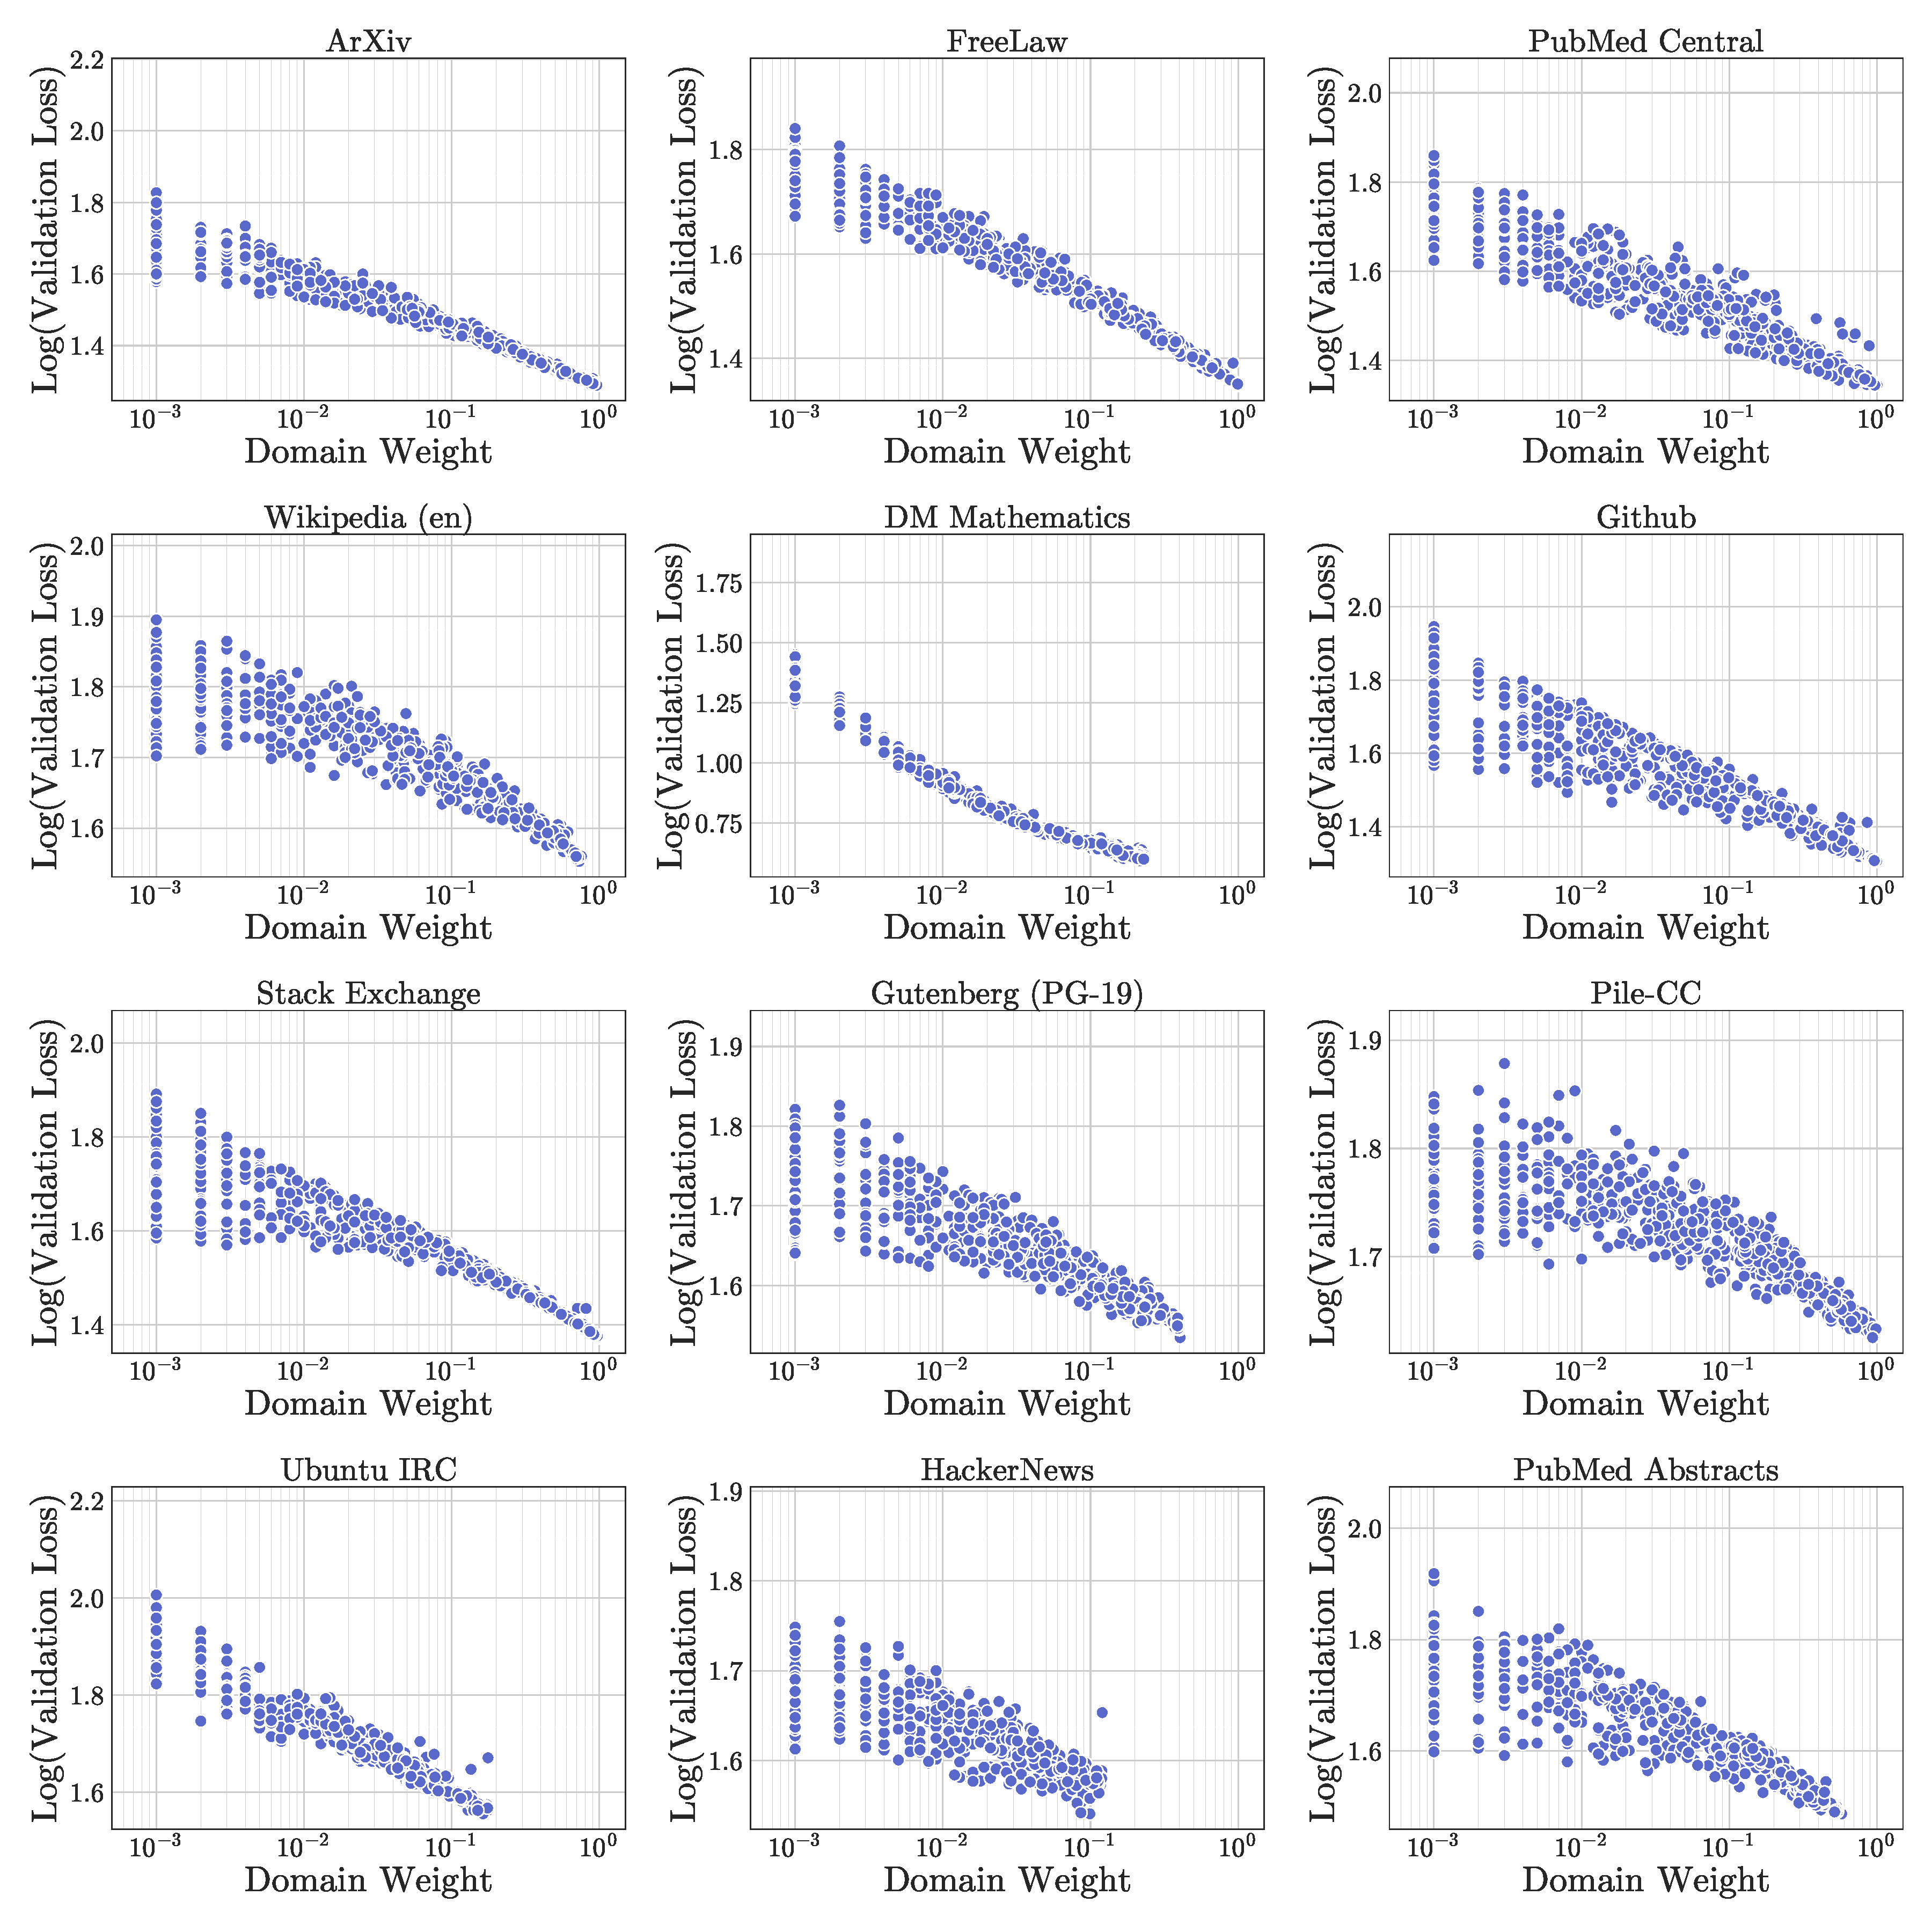
\includegraphics[width=1.0\textwidth]{figures/minimum_1024_log.pdf}
    \caption{The visualization of 1M training logs across various data mixture. The x-axis represents the weight of each domain in data mixture and the y-axis shows the log value of validation loss for that domain. As seen in the variation along the y-axis, predicting the validation loss solely based on the domain weight is challenging.}
    \label{fig:log_loss_vs_weight}
\end{figure}

Recent research~\citep{ye2024datamixing,ge2024data} has demonstrated the feasibility of scaling laws for data mixture.
However, our findings in Section~\ref{sec:domain_interaction} suggest that the relationship between domain weights and validation loss is more complex than scaling laws might imply.
To visualize this complexity, we plotted all experimental points of our 1M training logs in Figure~\ref{fig:log_loss_vs_weight}.
If the scaling law of data mixture held true, we would expect to see a clear log-log linear relationship across all domains.
However, our results reveal a more nuanced picture.
For example, the DM Mathematics domain, possibly due to its distinct distribution compared to other domains, exhibits a near log-log linear relationship between loss and domain weight.
In contrast, for most domains like Pile-CC show more complex patterns, where predicting validation loss is non-trivial.
As shown, domain interactions appear to be intricate, making it challenging to predict the validation loss for a domain based solely on its weight in the mixture.
These findings suggest that while scaling laws provide valuable insights, they may not fully capture the intricacies of data mixture dynamics.
Our approach addresses the challenge by modeling the entire data mixture as input for the regression model, providing a more comprehensive framework for understanding and predicting the validation loss while simultaneously accounting for all domain weights.

\section{Conclusion}

In this paper, we present a novel approach, \ourmethod, for automatically selecting the optimal data mixture for pre-training large language models. \ourmethod formulates the data mixture problem as a regression task and trains small models to predict the impact of different data mixtures. This enables efficient identification of the best mixture, which we then generalize to large-scale model training. \ourmethod predicts the best data mixture among 64 x 1B models demonstrating its effectiveness. Moreover, our large-scale study provides valuable insights into the impact of data mixture, the relationship between loss and downstream performance, and the domain interaction challenges for human experts in determining the optimal mixture.


\bibliography{ms}
\bibliographystyle{plainnat}

\clearpage
\appendix
\section{Limitations}
\label{sec:limitations}

Despite making progress in understanding and optimizing data mixtures for better performance, our method still has several limitations.

\paragraph{The maximum model parameters.} We have verified that small models can be used to predict the optimal data mixture for large-scale runs with up to 1B parameters. However, much larger models are commonly trained with 7B or 70B parameters~\citep{llama2paper}. Due to compute constraints we leave the verification of \ourmethod at larger scales to future work.

\paragraph{The benchmark coverage.} Owing to the scarcity of relevant data in the Pile corpus and the relatively small size of our model at 1B scale, their performance on the MMLU benchmark~\citep{MMLU2021} is nearly random and negligible on GSM8K~\citep{gsm8k2021}. Consequently, we do not compute the correlation between the validation loss and scores on these challenging benchmarks.


\paragraph{The infinite data assumption.} Most existing data mixing methods assume the availability of unlimited data for each domain. Although we consider this issue in our no Pile-CC experiments in Section~\ref{sec:no_pile_exper}, systematically incorporating the effect of available data into the method remains challenging. Combining our method with the decay coefficient of data reuse proposed in~\citet{muennighoff2023scaling} could be an interesting future work to explore, potentially addressing the limited data availability scenario.

\paragraph{The domain assumption.} 

A common assumption of existing data mixture methods (including ours) is that the domain each example belongs to is known. However, this may not always be the case and the domain needs to be obtained first. Assigning examples to domains is a hard task, which may make it challenging to apply our methods when the domain boundaries are unclear.

\paragraph{The tokenizer assumption.}

All existing data mixture methods require the use of proxy models to obtain domain weights. However, a fundamental assumption of these methods is that the proxy model uses the same tokenizer and vocabulary size as the large model. Generalizing weights across different tokenizers poses significant challenges.


\section{Ethic statements}
\label{sec:ethic}
Optimizing the data mixture for LLM pre-training raises several ethical issues. 
First, the optimized data mixture might be biased toward certain domains, which is good for achieving better performance. However, certain domains might be underrepresented or misrepresented, leading the trained models to perform poorly or produce biased results for these domains.
Second, though our method aims to optimize the data mixture efficiently, searching for the optimal data mixture still requires computational resources, leading to high energy consumption and environmental impact.
It is worthwhile to explore how to further reduce the computation cost. 



\clearpage
\section{Additional results}

\subsection{The regression prediction visualization}

As shown in Figure~\ref{fig:1M-to-128-1M-Joint}, we visualize the predicted and true loss pairs of the linear model and LightGBM model on the 1M models. 
The LightGBM model performs better than the linear model, achieving near 100\% Spearman Rank Correlation $\rho$.

\begin{figure}[t]
    \centering
    \subfigure{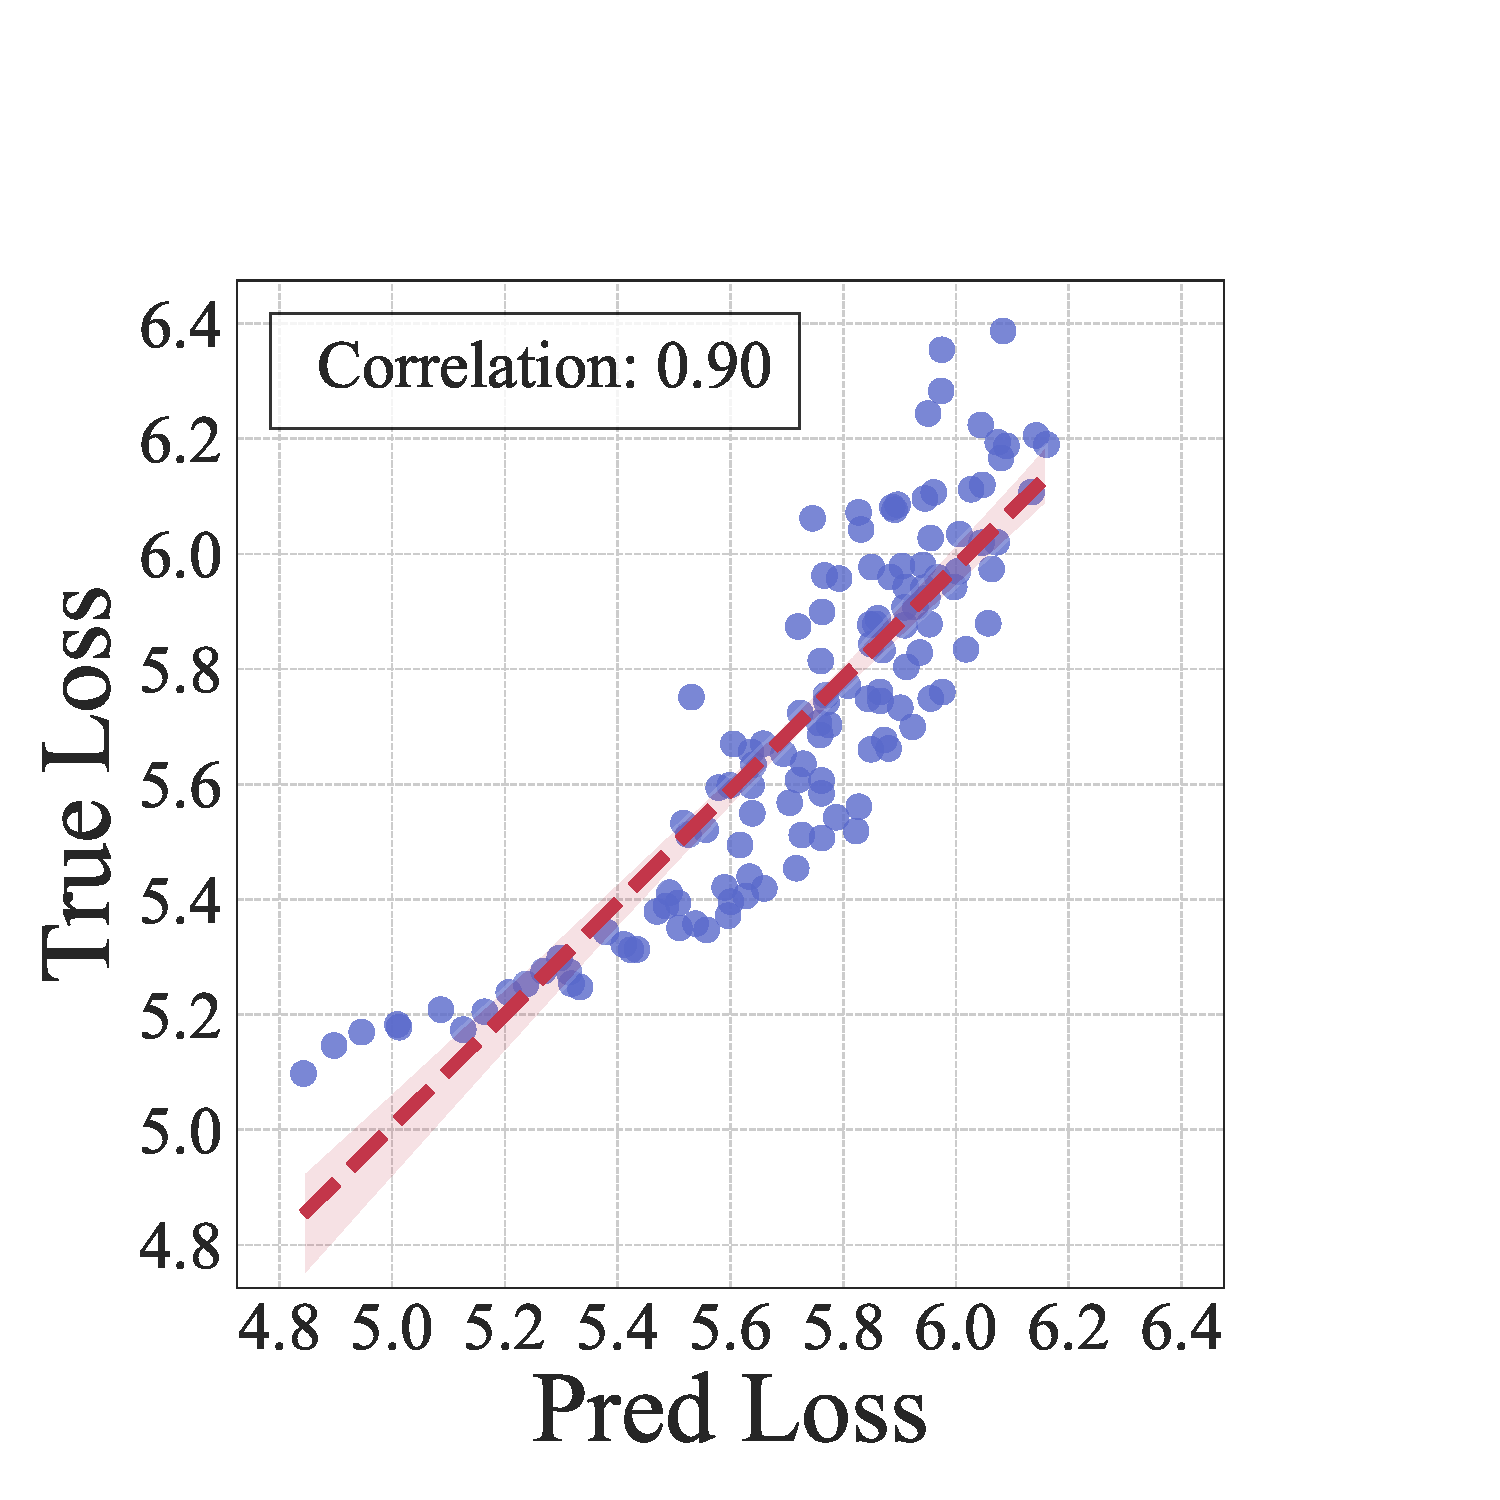
\includegraphics[width=0.45\textwidth]{figures/1M_pile_cc_Joint_linear.pdf}}
    \subfigure{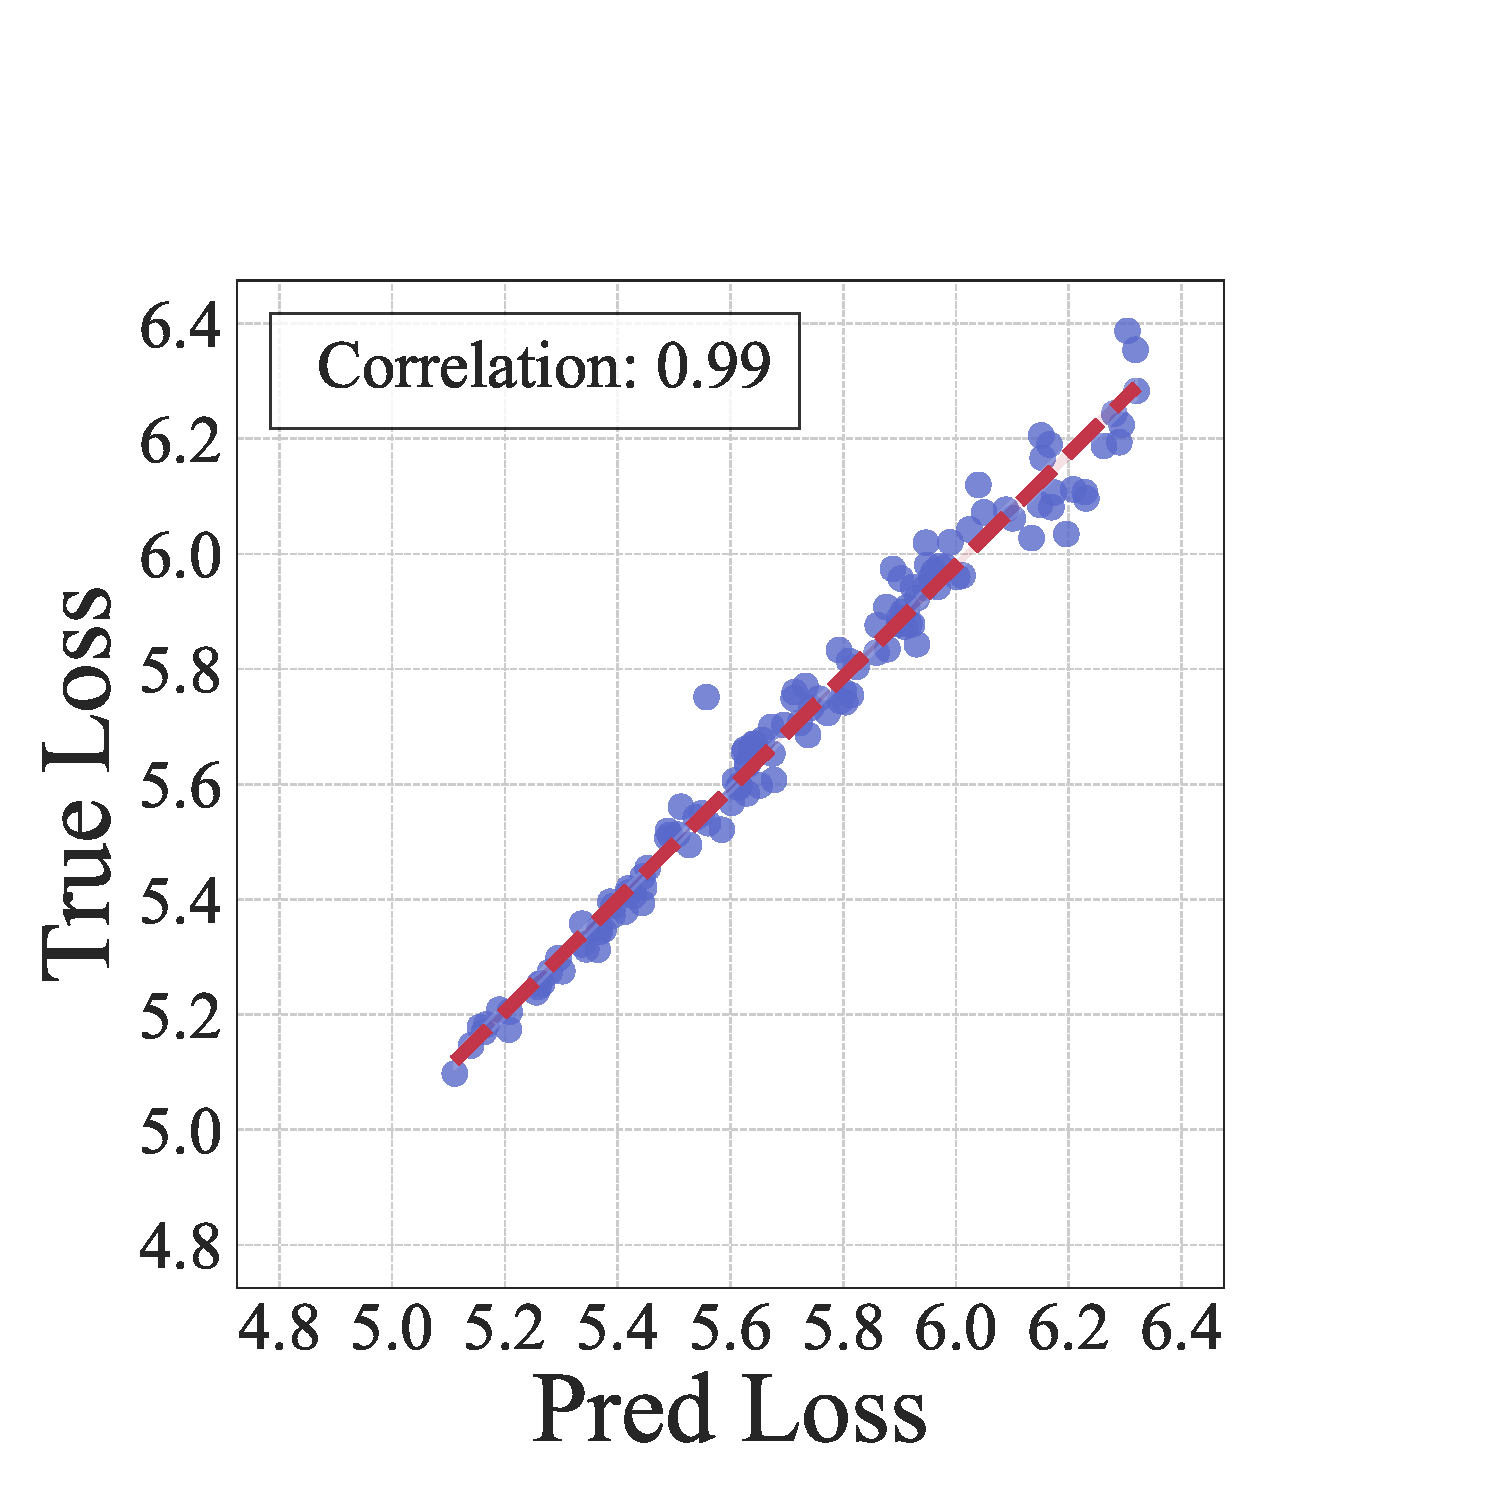
\includegraphics[width=0.45\textwidth]{figures/1M_pile_cc_Joint.pdf}}
    \caption{The visualization of loss prediction on small models (e.g., 1M parameters). \textbf{Left}: The scatter plot of predicted and true loss pairs of Linear model. \textbf{Right}: The scatter plot of predicted and true loss pairs of LightGBM model.}
    \label{fig:1M-to-128-1M-Joint}
\end{figure}


\subsection{Loss and rank prediction on small models for out-of-distribution setting}

In Section~\ref{sec:app}, we verify the effectiveness of our method in out-of-distribution scenarios where we fully exclude the Pile-CC domain from the pre-training corpus and use the remaining domains to find the optimal data mixture that minimizes Pile-CC validation loss. 
We also provide the results of regression evaluation under this setting in Figure~\ref{tab:linear_vs_lightgbm_1M_OOD}.
Similarly, LightGBM model outperforms the linear model and achieves nearly 100\% Spearman Rank Correlation $\rho$.

\begin{table}[htbp]
    \centering
    \small
    \caption{The regression model is fitted using the training artifacts of $512 \times$ 1M models trained with 1B tokens excluding the Pile-CC domain, and evaluated on \textbf{unseen data mixtures} for 1M parameter models. Pearson's r and MSE measure the loss prediction performance, while $\rho$ compares the predicted and actual ranks.}
    \label{tab:linear_vs_lightgbm_1M_OOD}
    \begin{tabular}{lccc}
        \toprule
        {Method} & \multicolumn{3}{c}{1M models with 1B tokens}\\
        \cmidrule(r){1-1} \cmidrule(lr){2-4}
        & $\rho$ ($\uparrow$) & 
        Pearson's $r$ ($\uparrow$) & MSE ($\downarrow$) \\
        \midrule
        Linear  & 83.00 & 84.18 & 0.08  \\
        LightGBM & \textbf{95.47} & \textbf{95.48} & \textbf{0.04} \\
        \bottomrule
    \end{tabular}
\end{table}

\subsection{The derived data mixtures}

Table~\ref{tab:data_mixture_all} presents the derived data mixture weights for different methods. As illustrated, \ourmethod assigns a high weight of 0.87 to the Pile-CC dataset, aligning with human intuition.


\begin{table}[t]
    \centering
    \caption{The domain weights of different methods. In our experiments, DoReMi refers to the reported best reference model with 280M parameters and its corresponding domain weights. $^\dagger$Note that the domain weights of Human and DoReMi are re-normalized from the weights reported in~\citet{xie2023doremi} to adapt them to the available domains. The DoReMi weight are derived from the best-performing configuration obtained using a 280M parameter model.}
    \label{tab:data_mixture_all}
\begin{threeparttable}
    \begin{tabular}{l|cccc}
    \toprule
        \textbf{Domain Weights} & \textbf{Human}$^\dagger$ & \textbf{DoReMi}$^\dagger$ & \textbf{Pile-CC Only} & \textbf{\ourmethod} \\
        \midrule
        ArXiv & 0.134  & 0.004  & 0.0 & 0.001 \\ 
        FreeLaw & 0.049  & 0.005  & 0.0 & 0.001 \\ 
        NIH ExPorter & 0.007  & 0.008  & 0.0 & 0.001 \\ 
        PubMed Central & 0.136  & 0.006  & 0.0 & 0.003 \\ 
        Wikipedia (en) & 0.117  & 0.086  & 0.0 & 0.016 \\ 
        DM Mathematics & 0.025  & 0.002  & 0.0 & 0.0 \\ 
        Github & 0.054  & 0.022  & 0.0 & 0.0 \\ 
        PhilPapers & 0.003  & 0.034  & 0.0 & 0.0 \\ 
        Stack Exchange & 0.118  & 0.019  & 0.0 & 0.0 \\ 
        Enron Emails & 0.004  & 0.009  & 0.0 & 0.002 \\ 
        Gutenberg (PG-19) & 0.025  & 0.009  & 0.0 & 0.002 \\ 
        Pile-CC & 0.142  & 0.743  & 1.0 & {0.87} \\ 
        Ubuntu IRC & 0.009  & 0.011  & 0.0 & {0.064} \\ 
        EuroParl & 0.005  & 0.008  & 0.0 & 0.0 \\ 
        HackerNews & 0.01  & 0.016  & 0.0 & {0.012} \\ 
        PubMed Abstracts & 0.107  & 0.014  & 0.0 & {0.024} \\ 
        USPTO Backgrounds & 0.053 & 0.004 & 0.0 & 0.002 \\
    \bottomrule
    \end{tabular}
    \end{threeparttable}
\end{table}

\subsection{The evaluation results using LightEval}\label{appendix:lighteval}


\begin{table}[tb]
    \centering
    \small
    \caption{Performance comparison of different data selection methods using LightEval following previous work~\citep{penedo2024finewebdatasetsdecantingweb}. Human refers to the weights put forth in The Pile~\citep{the_pile_corpus}, Pile-CC Only to only training on the Pile-CC component, and DoReMi to the weights from \citet{xie2023doremi}. The reported performance for each task is the average \textit{zero-shot task performance} across five different runs, and the standard deviation. We estimate the compute (measured in FLOPs) required to arrive at the training data mixture. Scores significantly outperforming the Human baseline for each task are highlighted in \textbf{bold}, with significance determined using Cohen's d. }
    \vspace{1mm}
    \label{tab:downstream_lighteval}
    \begin{tabular}{l|l|lll}
    \toprule
         \textbf{Benchmark} & \textbf{Human} & \textbf{DoReMi} & \textbf{Pile-CC Only} & \textbf{\ourmethod} \\
    \midrule
        ARC Easy~\citep{clark2018think} & 45.3\text{\,\scriptsize$\pm$\,0.4} &  {\textbf{46.6}}\text{\,\scriptsize$\pm$\,0.7} &  \textbf{47.1}\text{\,\scriptsize$\pm$\,0.6} & \textbf{47.2}\text{\,\scriptsize$\pm$\,0.9}  \\ 
        ARC Challenge~\citep{clark2018think} & 25.5\text{\,\scriptsize$\pm$\,0.8} & {25.9}\text{\,\scriptsize$\pm$\,0.8} & 25.6\text{\,\scriptsize$\pm$\,0.5} & 25.6\text{\,\scriptsize$\pm$\,0.5}  \\ 
        CommonsenseQA~\citep{talmor-etal-2019-commonsenseqa} & 31.8\text{\,\scriptsize$\pm$\,1.2} & {\textbf{34.1}}\text{\,\scriptsize$\pm$\,0.7} & \textbf{34.9}\text{\,\scriptsize$\pm$\,0.3} & \textbf{35.0}\text{\,\scriptsize$\pm$\,0.5}  \\ 
        HellaSwag~\citep{zellers2019hellaswag} & 36.5\text{\,\scriptsize$\pm$\,0.2} & \textbf{41.5}\text{\,\scriptsize$\pm$\,0.3} & \textbf{39.7}\text{\,\scriptsize$\pm$\,0.5} & \textbf{42.1}\text{\,\scriptsize$\pm$\,0.3}  \\ 
        OpenBookQA~\citep{mihaylov2018can} & {29.8}\text{\,\scriptsize$\pm$\,0.6} & \textbf{31.0}\text{\,\scriptsize$\pm$\,0.8} & \textbf{31.5}\text{\,\scriptsize$\pm$\,0.4} & \textbf{31.8}\text{\,\scriptsize$\pm$\,0.8}  \\ 
        PiQA~\citep{bisk2020piqa} &  65.4\text{\,\scriptsize$\pm$\,0.6} & \textbf{68.7}\text{\,\scriptsize$\pm$\,0.3} & \textbf{69.0}\text{\,\scriptsize$\pm$\,0.5} & \textbf{69.4}\text{\,\scriptsize$\pm$\,0.5}  \\ 
        Social IQA~\citep{sap2019socialiqa} & {41.7}\text{\,\scriptsize$\pm$\,0.3} &  42.0\text{\,\scriptsize$\pm$\,\,0.2} &  \textbf{42.7}\text{\,\scriptsize$\pm$\,0.3} &  \textbf{42.6}\text{\,\scriptsize$\pm$\,0.7}  \\ 
        WinoGrande~\citep{sakaguchi2021winogrande} & 51.1\text{\,\scriptsize$\pm$\,1.0}  & {51.2}\text{\,\scriptsize$\pm$\,0.4}  & 50.7\text{\,\scriptsize$\pm$\,1.0}  & {50.9}\text{\,\scriptsize$\pm$\,0.4}   \\ 
        MMLU~\citep{MMLU2021} & 28.6\text{\,\scriptsize$\pm$\,0.2}  & {28.9}\text{\,\scriptsize$\pm$\,0.4}  & 28.5\text{\,\scriptsize$\pm$\,0.2}  & {28.7}\text{\,\scriptsize$\pm$\,0.3}   \\ 
        \midrule
        Average Performance & 39.5\text{\,\scriptsize$\pm$\,0.3} & {41.1}\text{\,\scriptsize$\pm$\,0.3} & {41.2}\text{\,\scriptsize$\pm$\,0.3} & {41.5}\text{\,\scriptsize$\pm$\,0.2} \\
        Beat Human on & -- & 5 / 9 & 6 / 9 & 6 / 9 \\
        Estimated FLOPs & 0 & $3.7\times10^{19}$ & 0 & $3.5\times10^{18}$ \\
    \bottomrule
    \end{tabular}
\end{table}

Following the approach of FineWeb~\citep{penedo2024finewebdatasetsdecantingweb}, we employ the LightEval~\footnote{\url{https://github.com/huggingface/lighteval}} library to evaluate our models using a suite of benchmarks selected for their stability and suitability. The chosen benchmarks exhibit three key characteristics: low score variance across different data samples, monotonic score improvement during training, and above-random baseline scores for models in the 1B parameter range.
Table~\ref{tab:downstream_lighteval} presents the evaluation results. Our method, \ourmethod, consistently outperforms the Human baseline on 6 benchmarks. Moreover, \ourmethod demonstrates superior average performance compared to the DoReMi and the Pile-CC Only methods.



\clearpage
\section{URL domain correlation graph}\label{appendix:correaltion_graph}

\begin{figure}[htbp]
    \centering
    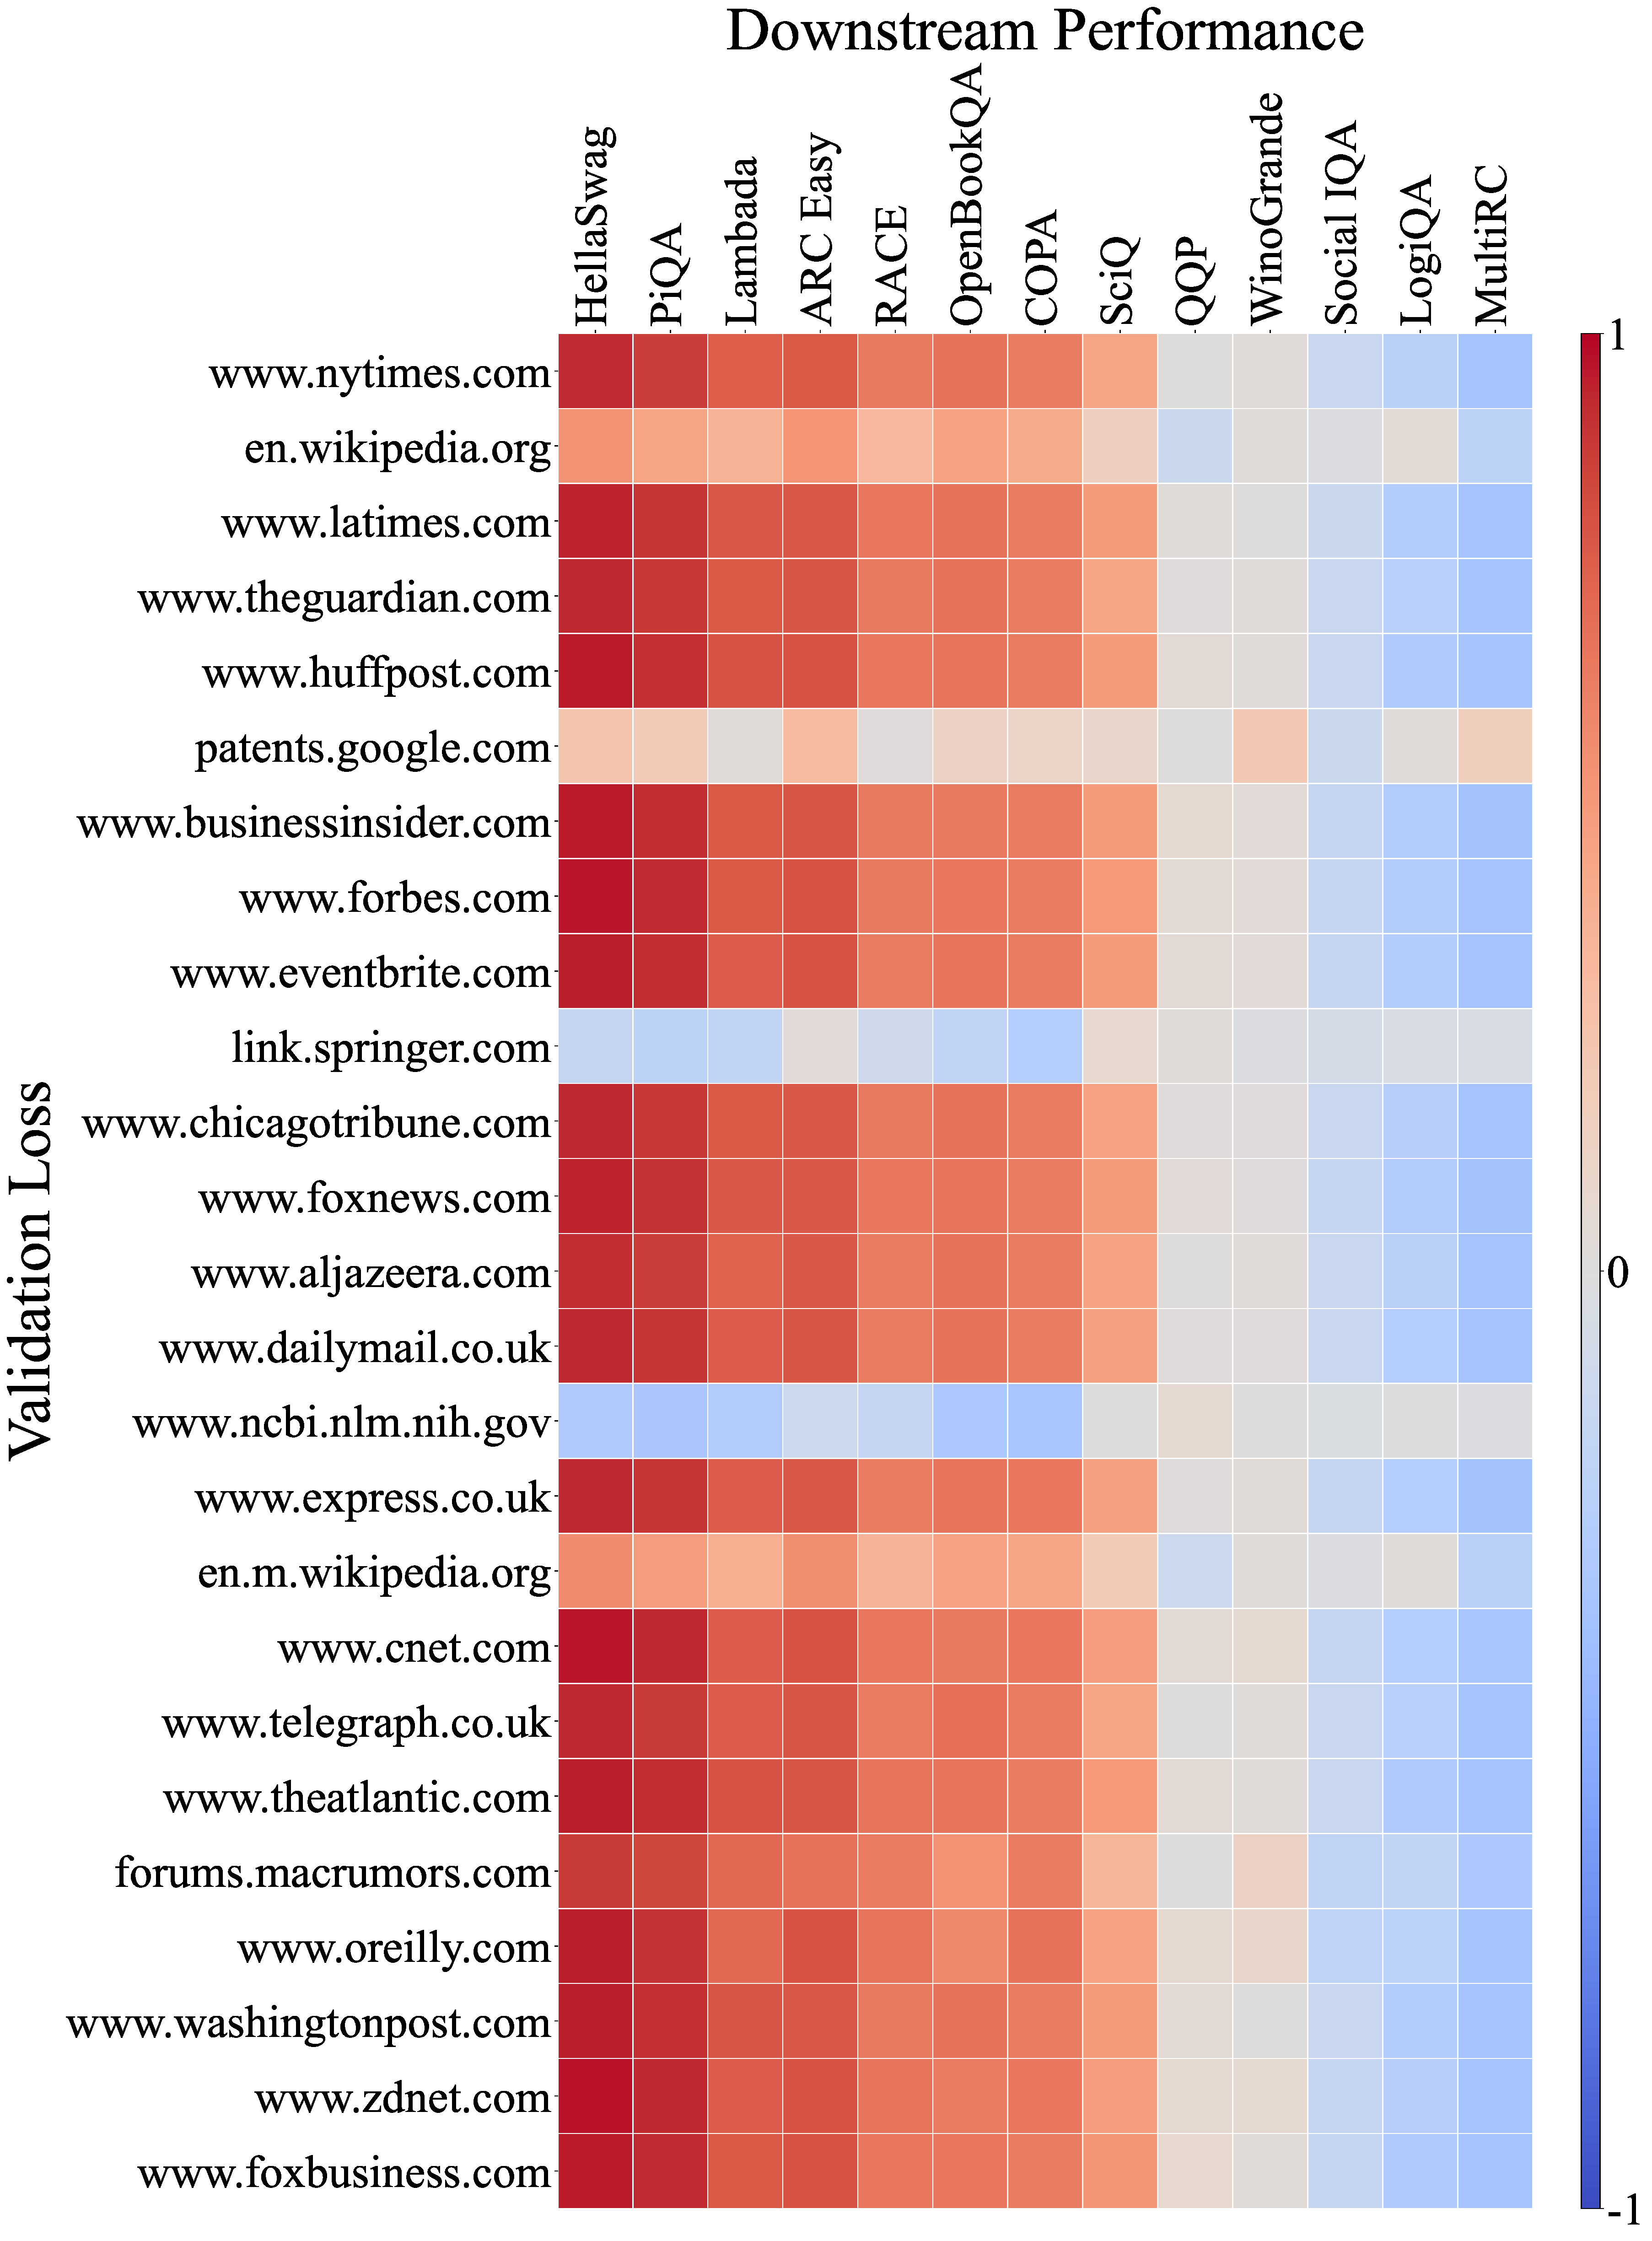
\includegraphics[height=0.9\textwidth]{figures/Domain_and_Task_c4100_full_1.pdf}
    \caption{The visualization of correlations between different URL domains within the C4 subsets and the downstream performance (Part 1).}
    \label{fig:c4100-full-1}
\end{figure}

\begin{figure}[htbp]
    \centering
    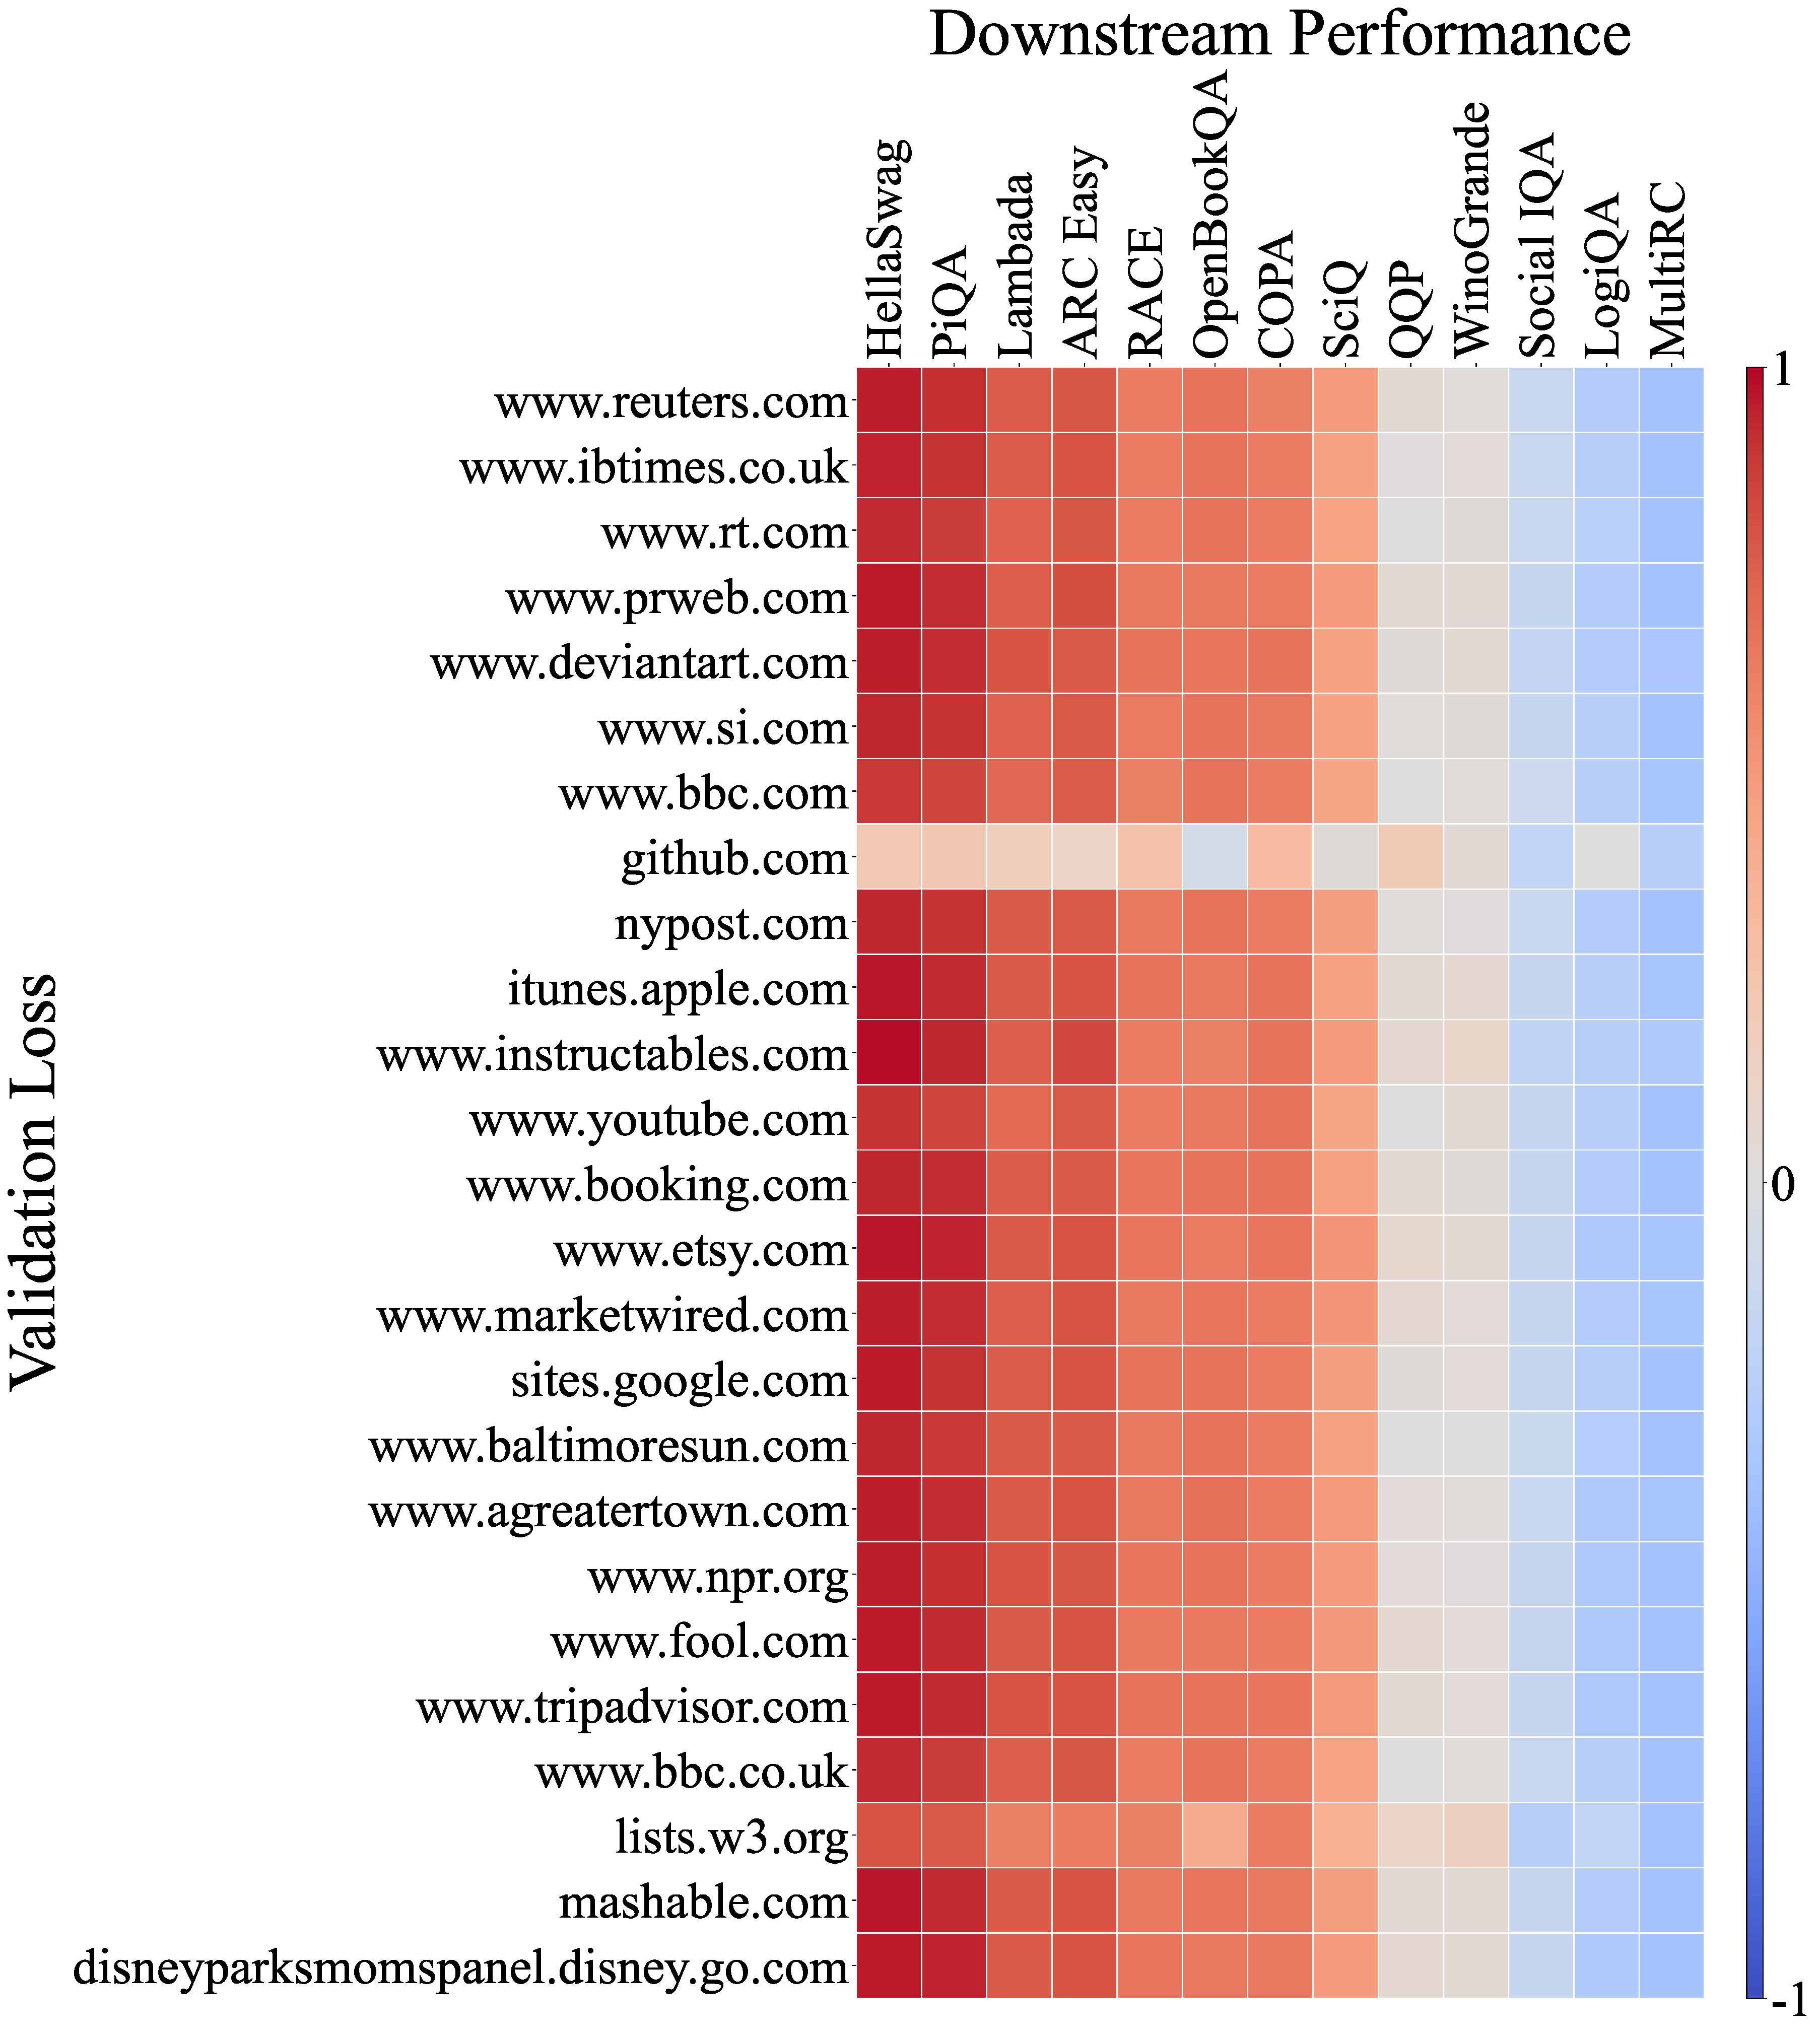
\includegraphics[height=0.9\textwidth]{figures/Domain_and_Task_c4100_full_2.pdf}
    \caption{The visualization of correlations between different URL domains within the C4 subsets and the downstream performance (Part 2).}
    \label{fig:c4100-full-2}
\end{figure}

\begin{figure}[htbp]
    \centering
    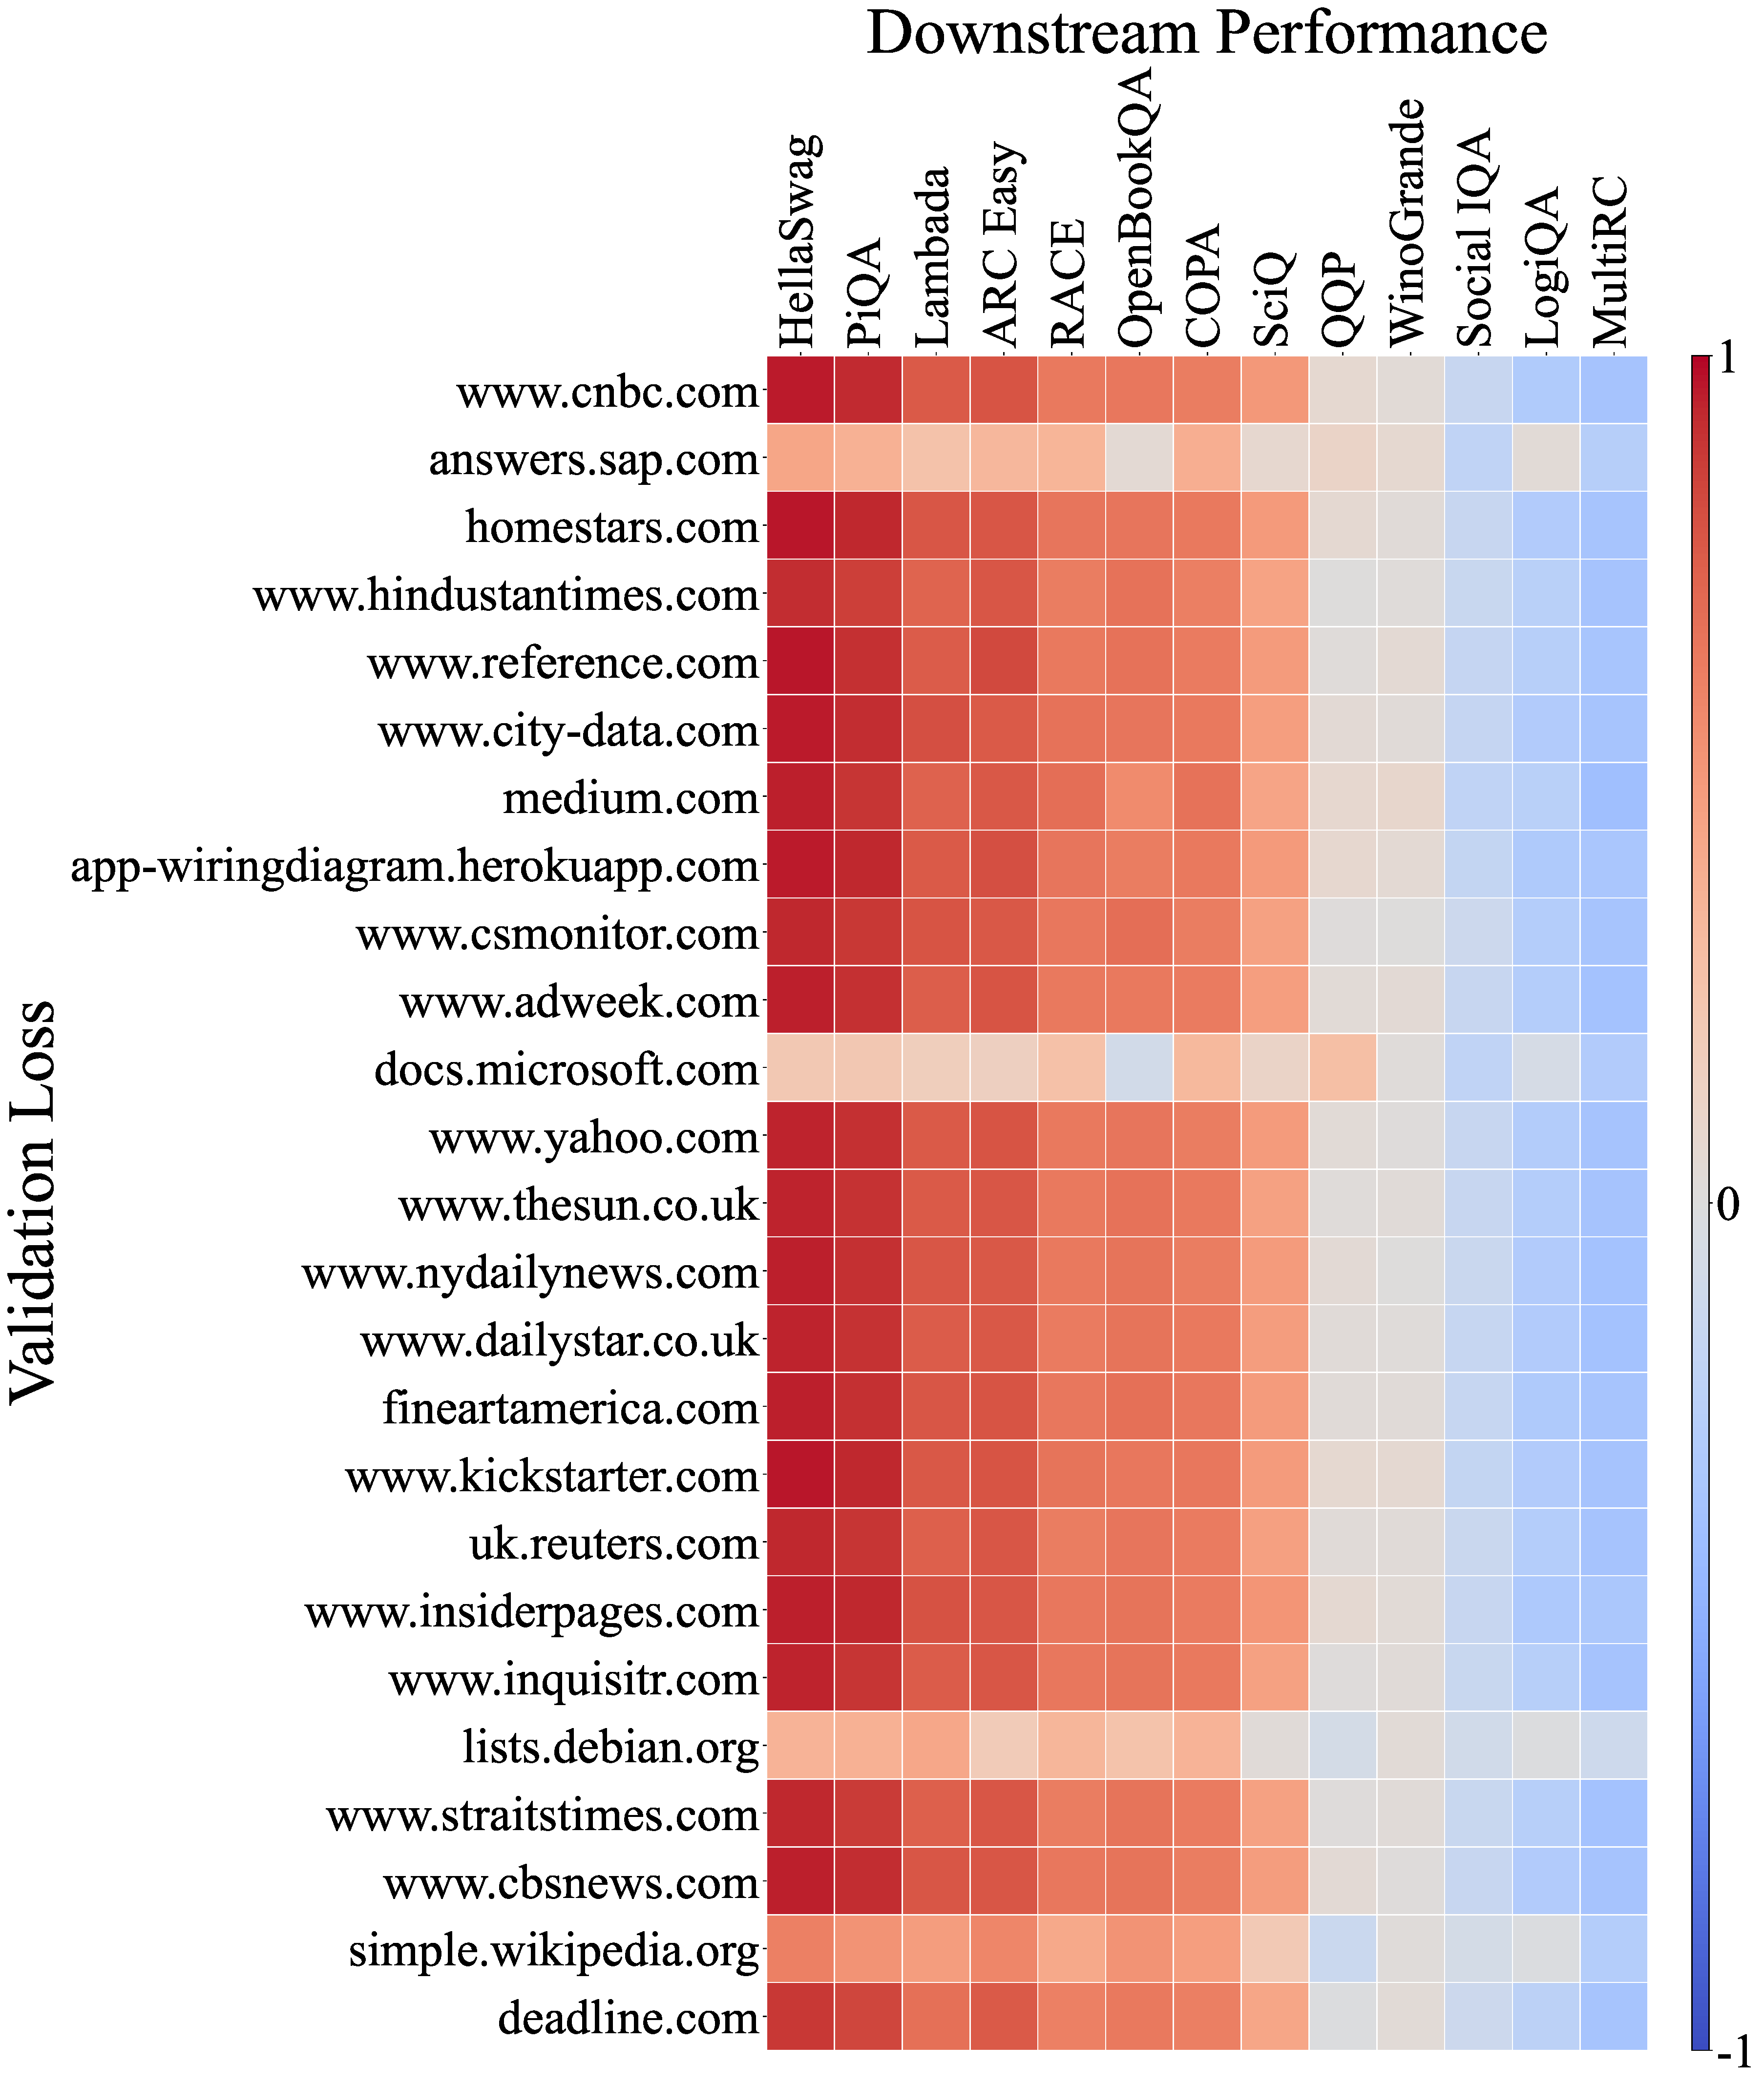
\includegraphics[height=0.9\textwidth]{figures/Domain_and_Task_c4100_full_3.pdf}
    \caption{The visualization of correlations between different URL domains within the C4 subsets and the downstream performance (Part 3).}
    \label{fig:c4100-full-3}
\end{figure}

\begin{figure}[htbp]
    \centering
    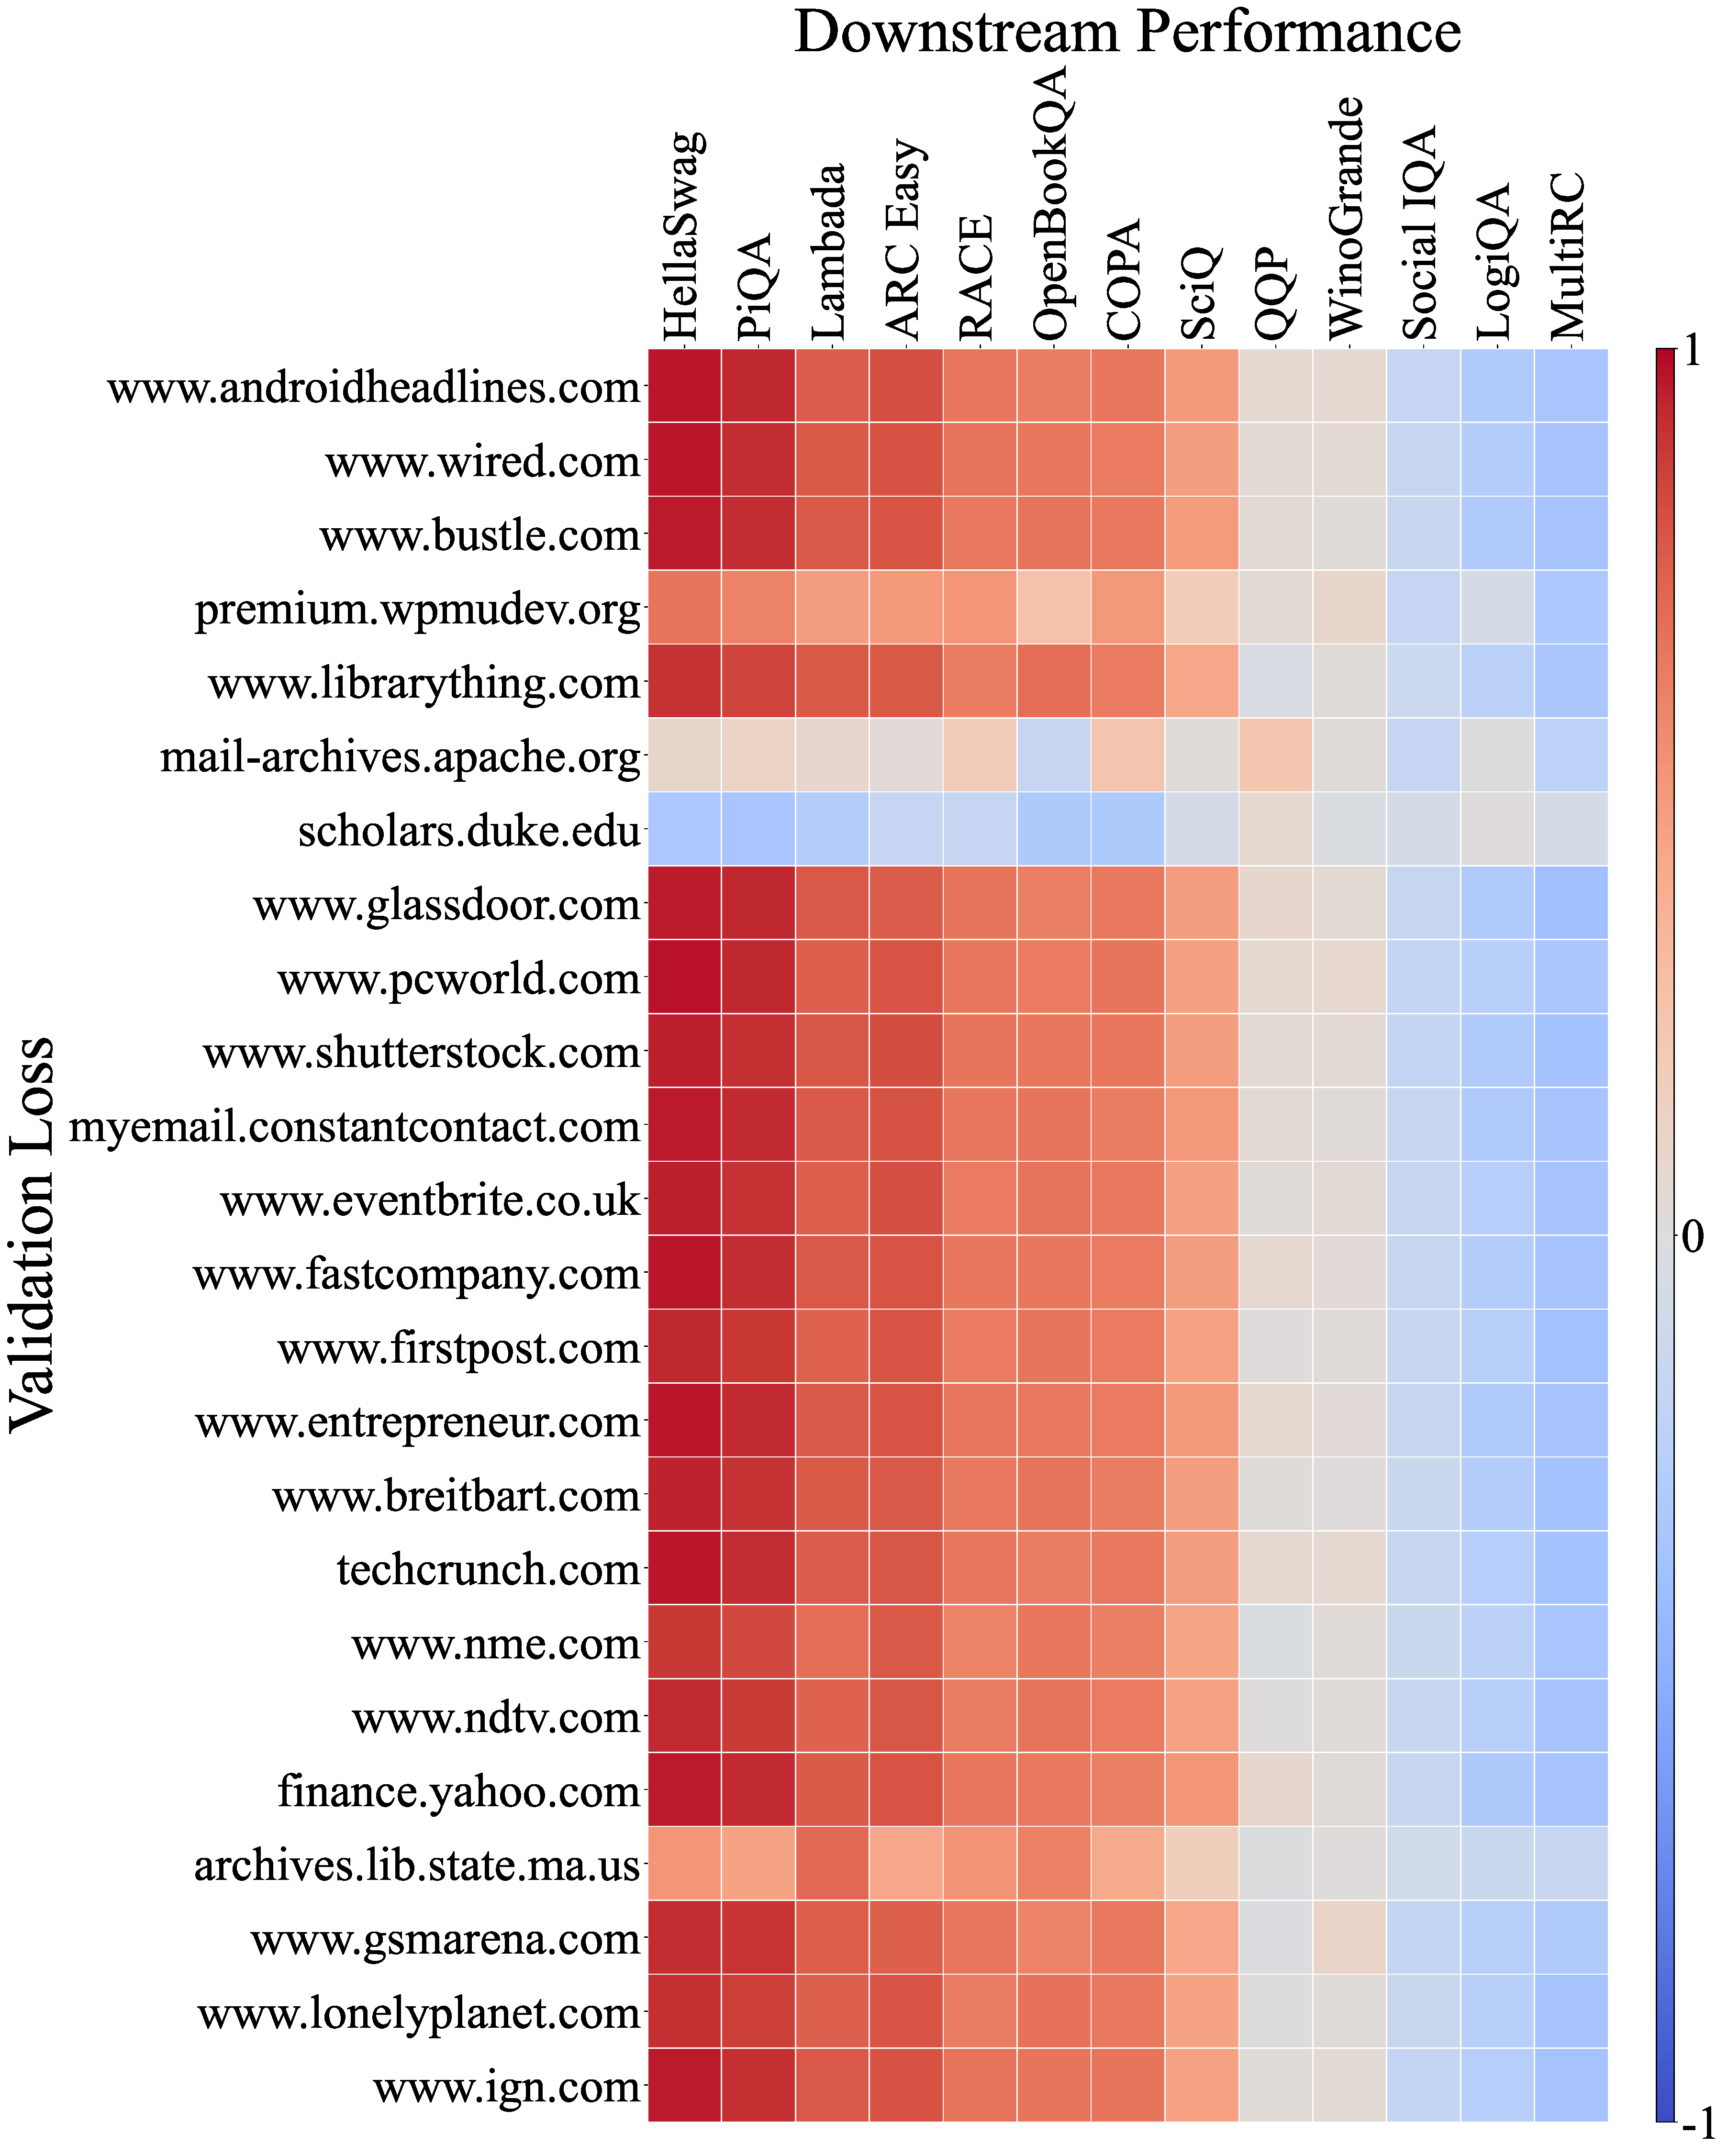
\includegraphics[height=0.9\textwidth]{figures/Domain_and_Task_c4100_full_4.pdf}
    \caption{The visualization of correlations between different URL domains within the C4 subsets and the downstream performance (Part 4).}
    \label{fig:c4100-full-4}
\end{figure}


\clearpage
\section{Implementation details}
\label{appendix:implement}
We utilize the model architecture proposed by \citet{zhang2024tinyllama} and create various model variants by modifying the number of layers, the number of attention heads, and the dimensions of token embeddings and hidden states, as illustrated in Figure~\ref{tab:model_config}.
For tokenization, we employ the GPTNeoX tokenizer \citep{black2022gpt}, which has a vocabulary size of 50,432.

For models with 1M and 60M parameters, we set the training iterations as 1000 and the batch size as 1M tokens, which means the training budget is 1B tokens.
Similarly, we train the larger model with 1B parameters with 25000 training iterations and the same batch size thus consuming 25B tokens in total.
We set the learning rate as 4e-4 and use the cosine learning rate scheduler.

For linear regression, we employ 5-fold cross-validation with ridge regression to determine the optimal $\ell_2$ regularization weight from the set [1e-3, 1e-2, 1e-1, 1e0, 1e1, 1e2, 1e3].
For LightGBM, we manually set the number of iterations to 1000 and the learning rate to 1e-2.
leaving all other hyperparameters at their default values.



\begin{table}[htbp]
    \centering
    \caption{The detailed model configuration for different model sizes.}
    \label{tab:model_config}
    \begin{tabular}{cccc}
        \toprule
        \textbf{Model} & \textbf{1M} & \textbf{60M} & \textbf{1B} \\
        \midrule
        Vocabulary Size & 50432 & 50432 & 50432 \\
        $n_{\rm layers}$ & 2 & 10 & 22 \\
        $n_{\rm heads}$ & 8 & 8 & 16 \\
        $d_{\rm embedding}$ & 256 & 768 & 2048 \\
        $d_{\rm model}$ & 512 & 1536 & 5632 \\
        \bottomrule
    \end{tabular}
\end{table}
\section{The stability of our method}\label{appendix:stability}

\begin{figure}[tb]
    \centering
    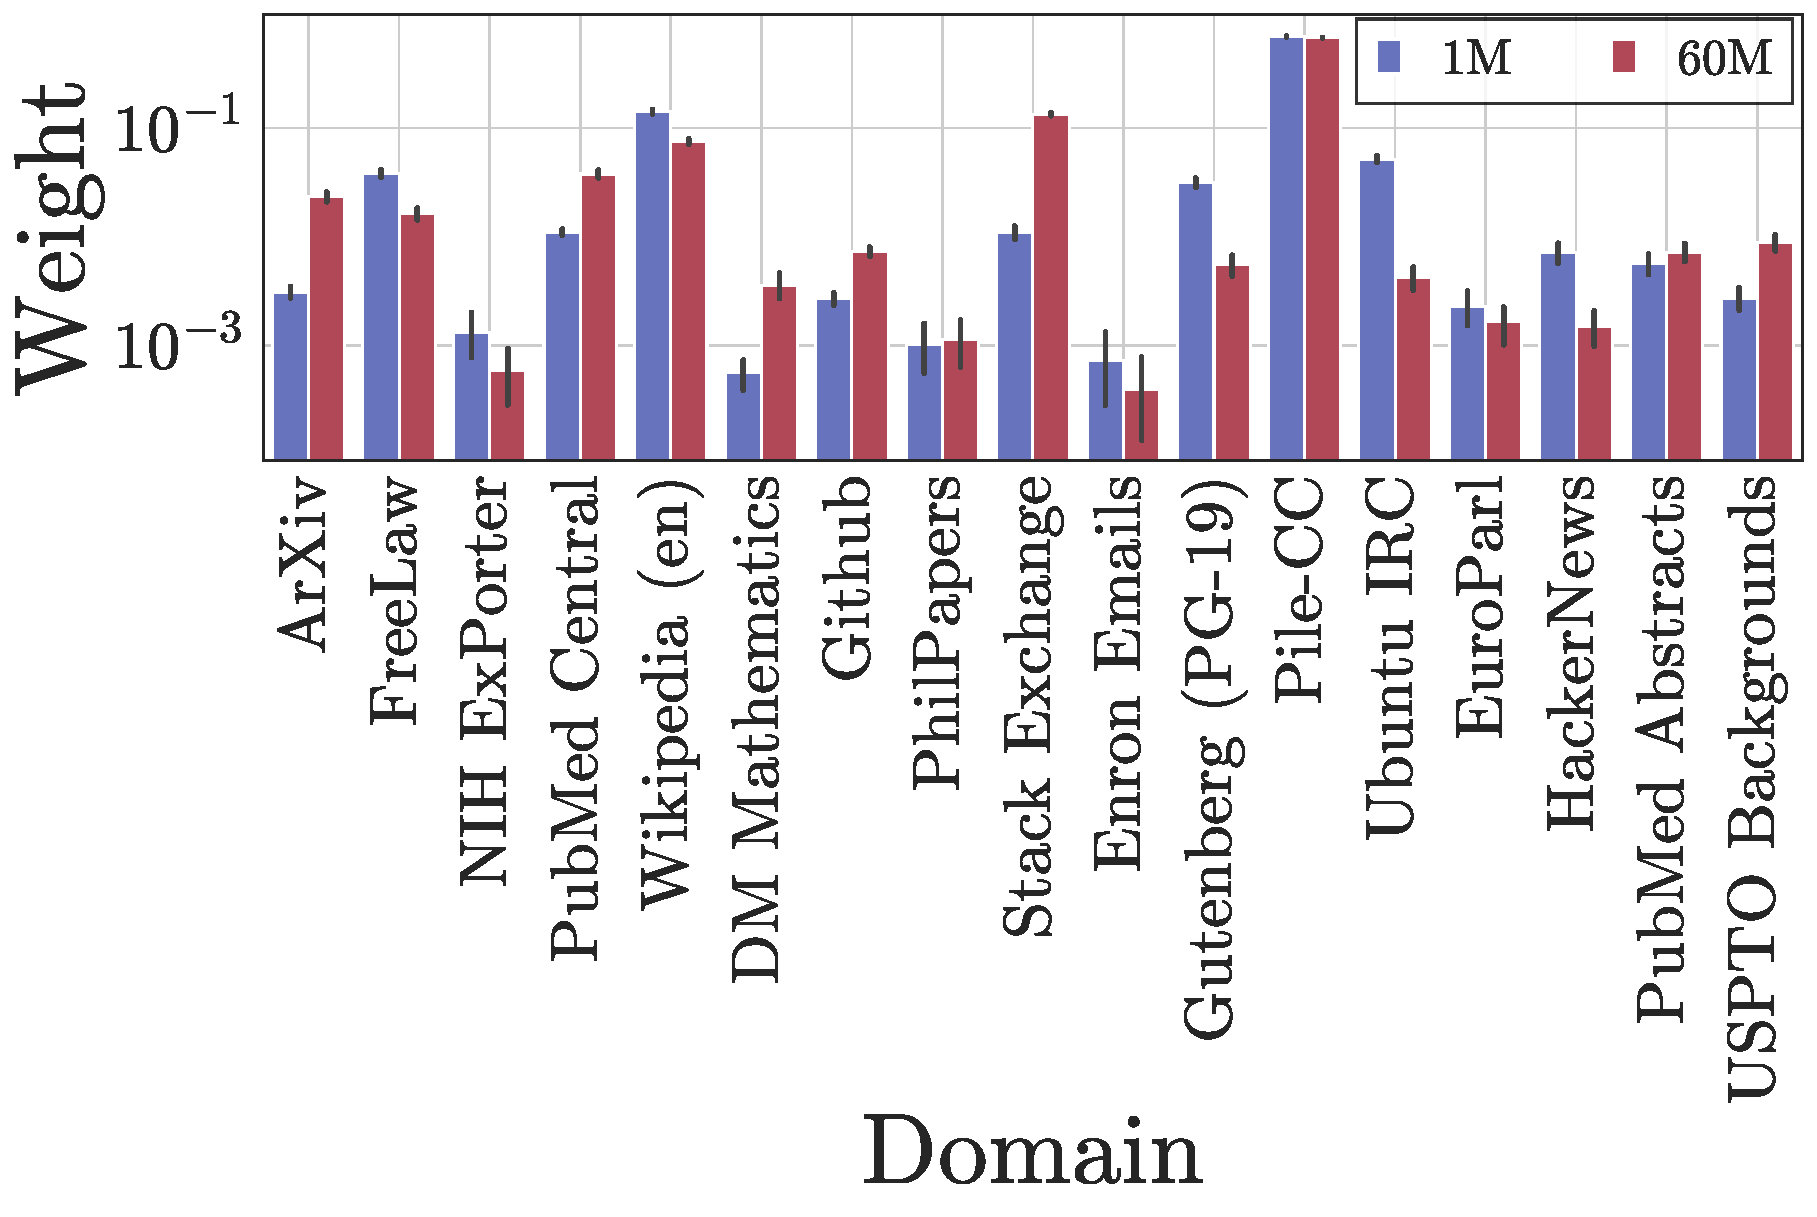
\includegraphics[width=0.5\textwidth]{figures/1M_vs_60M.pdf}
    \caption{\ourmethod yields similar data mixture distributions when using the 1M model and the 60M model as proxy models, demonstrating the stability of our method. Note that the y-axis is in log-scale for visualization purpose.}
    \label{fig:robustness_ours}
\end{figure}

Previous research~\citep{xie2023doremi,fan2023doge,albalak2023efficient} has employed small-scale proxy models, trained on substantial volumes of tokens, to predict optimal data mixtures for large language models.
However, these approaches often suffer from instability issues.
For example, DoReMi~\citep{xie2023doremi} reported that different proxy model sizes can result in significantly different predicted data mixtures.
Their findings (Figure 8, Appendix) show that using a 280M proxy model resulted in a Pile-CC weight of 0.67, while a 1B proxy model yielded a Pile-CC weight below 0.20.
The large discrepancy highlights potential instabilities in previous approaches.
To evaluate the robustness of \ourmethod against such instabilities, we conducted comparative experiments using two distinct model scales: a 1M proxy model and a 60M proxy model. We used their respective training logs to fit regression models and subsequently simulated the top 1024 predictions. The resulting distributions are plotted in Figure~\ref{fig:robustness_ours}.
Our results demonstrate that while the prediction distributions for the 1M and 60M models are not identical, they exhibit remarkably similar patterns. This consistency suggests that \ourmethod achieves improved stability compared to previous approaches, even when varying the scale of proxy training models.


\section{Detailed experimental results}\label{appendix:all_model_results}

To facilitate future research, we share all the data mixtures and the corresponding downstream performances of the 64 trained models with 1B parameters.

\begin{table}[!ht]
    \centering
    \begin{tabular}{lllllllll}
    \toprule
        \textbf{Model Index} & \textbf{1} & \textbf{2} & \textbf{3} & \textbf{4} & \textbf{5} & \textbf{6} & \textbf{7} & \textbf{8} \\ 
        \midrule
        \multicolumn{9}{c}{\textit{Pre-training Domain Weights}} \\
        ArXiv & 0.123 & 0.066 & 0.055 & 0.059 & 0.201 & 0.036 & 0.042 & 0.126 \\ 
        FreeLaw & 0.065 & 0.071 & 0.052 & 0.083 & 0.004 & 0.212 & 0.113 & 0.21 \\ 
        NIH ExPorter & 0.0 & 0.0 & 0.004 & 0.0 & 0.014 & 0.0 & 0.0 & 0.0 \\ 
        PubMed Central & 0.126 & 0.211 & 0.177 & 0.174 & 0.243 & 0.153 & 0.089 & 0.123 \\ 
        Wikipedia (en) & 0.036 & 0.013 & 0.02 & 0.177 & 0.01 & 0.005 & 0.022 & 0.055 \\ 
        DM Mathematics & 0.0 & 0.0 & 0.011 & 0.0 & 0.03 & 0.047 & 0.007 & 0.008 \\ 
        Github & 0.034 & 0.153 & 0.095 & 0.194 & 0.017 & 0.205 & 0.028 & 0.008 \\ 
        PhilPapers & 0.0 & 0.033 & 0.0 & 0.0 & 0.0 & 0.0 & 0.0 & 0.0 \\ 
        Stack Exchange & 0.039 & 0.097 & 0.18 & 0.0 & 0.103 & 0.075 & 0.011 & 0.129 \\ 
        Enron Emails & 0.0 & 0.0 & 0.0 & 0.0 & 0.0 & 0.0 & 0.0 & 0.0 \\ 
        Gutenberg (PG-19) & 0.0 & 0.0 & 0.016 & 0.0 & 0.002 & 0.0 & 0.217 & 0.035 \\ 
        Pile-CC & 0.27 & 0.101 & 0.381 & 0.192 & 0.359 & 0.209 & 0.232 & 0.288 \\ 
        Ubuntu IRC & 0.0 & 0.0 & 0.001 & 0.005 & 0.0 & 0.0 & 0.08 & 0.0 \\ 
        EuroParl & 0.0 & 0.0 & 0.0 & 0.109 & 0.0 & 0.001 & 0.117 & 0.0 \\ 
        HackerNews & 0.0 & 0.011 & 0.005 & 0.0 & 0.0 & 0.0 & 0.018 & 0.0 \\ 
        PubMed Abstracts & 0.0 & 0.136 & 0.0 & 0.005 & 0.014 & 0.002 & 0.011 & 0.016 \\ 
        USPTO Backgrounds & 0.307 & 0.106 & 0.003 & 0.0 & 0.002 & 0.055 & 0.011 & 0.0 \\
        \midrule
        \multicolumn{9}{c}{\textit{Downstream Performance (\%)}} \\
        Social IQA & 33.27 & 33.33 & 33.62 & 33.53 & 33.49 & 33.56 & 33.62 & 33.55 \\ 
        HellaSwag & 40.58 & 36.86 & 40.58 & 36.06 & 40.07 & 37.85 & 37.93 & 39.59 \\ 
        PiQA & 67.29 & 65.14 & 67.97 & 64.66 & 67.03 & 65.36 & 66.0 & 66.55 \\ 
        OpenBookQA & 28.63 & 27.87 & 29.33 & 29.1 & 29.23 & 28.33 & 29.13 & 28.73 \\ 
        Lambada & 29.17 & 26.86 & 31.55 & 27.11 & 29.16 & 28.92 & 31.53 & 30.92 \\ 
        SciQ & 80.68 & 79.98 & 81.05 & 80.8 & 82.4 & 79.88 & 78.67 & 79.7 \\ 
        COPA & 70.5 & 63.83 & 69.17 & 65.0 & 67.5 & 66.0 & 66.67 & 68.67 \\ 
        RACE & 29.47 & 30.0 & 32.11 & 28.82 & 31.13 & 30.06 & 29.9 & 30.75 \\ 
        ARC Easy & 50.03 & 48.72 & 50.01 & 46.64 & 51.06 & 47.46 & 46.75 & 48.39 \\ 
        LogiQA & 23.76 & 24.17 & 25.29 & 25.29 & 24.55 & 25.96 & 25.45 & 26.32 \\ 
        QQP & 55.71 & 55.9 & 54.84 & 56.52 & 54.01 & 56.34 & 52.35 & 54.2 \\ 
        WinoGrande & 51.54 & 51.59 & 51.39 & 50.91 & 53.13 & 52.26 & 51.26 & 51.45 \\ 
        MultiRC & 52.65 & 53.39 & 51.89 & 50.92 & 49.03 & 53.09 & 53.64 & 50.23 \\
        \midrule
        \textbf{Avg} & 47.18 & 45.97 & 47.60 & 45.80 & 47.06 & 46.54 & 46.38 & 46.85 \\ \bottomrule
    \end{tabular}
\end{table}



\begin{table}[!ht]
    \centering
    \begin{tabular}{lllllllll}
    \toprule
        \textbf{Model Index} & \textbf{9} & \textbf{10} & \textbf{11} & \textbf{12} & \textbf{13} & \textbf{14} & \textbf{15} & \textbf{16} \\
        \midrule
        \multicolumn{9}{c}{\textit{Pre-training Domain Weights}} \\
        ArXiv & 0.184 & 0.226 & 0.107 & 0.139 & 0.101 & 0.099 & 0.251 & 0.147 \\ 
        FreeLaw & 0.009 & 0.046 & 0.276 & 0.048 & 0.047 & 0.002 & 0.024 & 0.046 \\ 
        NIH ExPorter & 0.0 & 0.0 & 0.0 & 0.0 & 0.001 & 0.022 & 0.0 & 0.0 \\ 
        PubMed Central & 0.094 & 0.261 & 0.157 & 0.184 & 0.119 & 0.501 & 0.101 & 0.196 \\ 
        Wikipedia (en) & 0.035 & 0.001 & 0.009 & 0.032 & 0.049 & 0.003 & 0.17 & 0.14 \\ 
        DM Mathematics & 0.007 & 0.001 & 0.0 & 0.001 & 0.092 & 0.0 & 0.0 & 0.008 \\ 
        Github & 0.106 & 0.189 & 0.024 & 0.055 & 0.078 & 0.017 & 0.048 & 0.237 \\ 
        PhilPapers & 0.0 & 0.0 & 0.0 & 0.0 & 0.0 & 0.043 & 0.019 & 0.0 \\ 
        Stack Exchange & 0.142 & 0.077 & 0.051 & 0.109 & 0.002 & 0.065 & 0.007 & 0.06 \\ 
        Enron Emails & 0.0 & 0.0 & 0.0 & 0.0 & 0.0 & 0.0 & 0.0 & 0.0 \\ 
        Gutenberg (PG-19) & 0.0 & 0.01 & 0.001 & 0.0 & 0.051 & 0.091 & 0.0 & 0.012 \\ 
        Pile-CC & 0.341 & 0.114 & 0.273 & 0.354 & 0.283 & 0.055 & 0.339 & 0.111 \\ 
        Ubuntu IRC & 0.0 & 0.003 & 0.0 & 0.0 & 0.057 & 0.0 & 0.017 & 0.0 \\ 
        EuroParl & 0.0 & 0.0 & 0.003 & 0.003 & 0.0 & 0.006 & 0.0 & 0.0 \\ 
        HackerNews & 0.002 & 0.0 & 0.034 & 0.0 & 0.0 & 0.0 & 0.0 & 0.001 \\ 
        PubMed Abstracts & 0.005 & 0.039 & 0.009 & 0.075 & 0.061 & 0.007 & 0.0 & 0.01 \\ 
        USPTO Backgrounds & 0.075 & 0.033 & 0.056 & 0.0 & 0.057 & 0.088 & 0.024 & 0.032 \\
        \midrule
        \multicolumn{9}{c}{\textit{Downstream Performance (\%)}} \\
        Social IQA & 33.43 & 33.21 & 33.31 & 33.17 & 33.28 & 32.43 & 33.57 & 33.7 \\ 
        HellaSwag & 40.05 & 35.89 & 39.55 & 39.89 & 38.63 & 36.18 & 39.52 & 35.94 \\ 
        PiQA & 66.6 & 64.74 & 66.29 & 66.27 & 66.9 & 64.05 & 66.7 & 64.51 \\ 
        OpenBookQA & 28.87 & 26.6 & 29.33 & 28.73 & 29.4 & 27.87 & 29.67 & 27.83 \\ 
        Lambada & 31.39 & 27.37 & 30.32 & 30.31 & 31.38 & 26.25 & 29.86 & 26.95 \\ 
        SciQ & 81.1 & 79.12 & 79.97 & 82.85 & 79.42 & 81.4 & 81.38 & 81.23 \\ 
        COPA & 67.0 & 64.5 & 66.83 & 69.5 & 67.33 & 65.83 & 69.5 & 66.33 \\ 
        RACE & 30.57 & 29.63 & 30.49 & 30.85 & 30.35 & 28.66 & 31.21 & 29.57 \\ 
        ARC Easy & 50.66 & 47.74 & 47.47 & 50.18 & 49.92 & 49.52 & 50.73 & 48.65 \\ 
        LogiQA & 23.6 & 25.65 & 26.37 & 23.81 & 25.58 & 26.29 & 25.86 & 25.12 \\ 
        QQP & 54.89 & 54.79 & 54.2 & 55.23 & 53.69 & 57.09 & 53.95 & 54.24 \\ 
        WinoGrande & 50.83 & 51.84 & 51.05 & 51.83 & 52.12 & 52.0 & 51.01 & 51.82 \\ 
        MultiRC & 54.18 & 54.48 & 50.17 & 52.12 & 51.42 & 52.69 & 51.87 & 53.48 \\ 
        \midrule
        \textbf{Avg} & 47.17 & 45.81 & 46.57 & 47.29 & 46.88 & 46.17 & 47.30 & 46.11 \\ \bottomrule    
        \end{tabular}
\end{table}

\begin{table}[!ht]
    \centering
    \begin{tabular}{lllllllll}
    \toprule
        \textbf{Model Index} & \textbf{17} & \textbf{18} & \textbf{19} & \textbf{20} & \textbf{21} & \textbf{22} & \textbf{23} & \textbf{24} \\
        \midrule
        \multicolumn{9}{c}{\textit{Pre-training Domain Weights}} \\
        ArXiv & 0.228 & 0.0 & 0.501 & 0.101 & 0.047 & 0.031 & 0.078 & 0.068 \\ 
        FreeLaw & 0.016 & 0.019 & 0.005 & 0.03 & 0.014 & 0.073 & 0.024 & 0.181 \\ 
        NIH ExPorter & 0.0 & 0.0 & 0.0 & 0.0 & 0.0 & 0.0 & 0.0 & 0.0 \\ 
        PubMed Central & 0.204 & 0.084 & 0.156 & 0.272 & 0.163 & 0.053 & 0.302 & 0.126 \\ 
        Wikipedia (en) & 0.02 & 0.159 & 0.17 & 0.021 & 0.218 & 0.129 & 0.027 & 0.07 \\ 
        DM Mathematics & 0.036 & 0.009 & 0.0 & 0.099 & 0.0 & 0.0 & 0.0 & 0.001 \\ 
        Github & 0.02 & 0.012 & 0.022 & 0.124 & 0.137 & 0.066 & 0.04 & 0.195 \\ 
        PhilPapers & 0.004 & 0.0 & 0.017 & 0.0 & 0.0 & 0.0 & 0.0 & 0.0 \\ 
        Stack Exchange & 0.002 & 0.052 & 0.062 & 0.113 & 0.173 & 0.12 & 0.007 & 0.24 \\ 
        Enron Emails & 0.0 & 0.0 & 0.0 & 0.0 & 0.0 & 0.0 & 0.0 & 0.0 \\ 
        Gutenberg (PG-19) & 0.0 & 0.001 & 0.002 & 0.054 & 0.001 & 0.089 & 0.002 & 0.0 \\ 
        Pile-CC & 0.244 & 0.361 & 0.061 & 0.154 & 0.19 & 0.057 & 0.499 & 0.023 \\ 
        Ubuntu IRC & 0.0 & 0.296 & 0.002 & 0.0 & 0.029 & 0.001 & 0.0 & 0.0 \\ 
        EuroParl & 0.004 & 0.0 & 0.0 & 0.001 & 0.007 & 0.0 & 0.0 & 0.0 \\ 
        HackerNews & 0.0 & 0.0 & 0.0 & 0.0 & 0.011 & 0.031 & 0.0 & 0.0 \\ 
        PubMed Abstracts & 0.196 & 0.001 & 0.0 & 0.011 & 0.008 & 0.351 & 0.0 & 0.059 \\ 
        USPTO Backgrounds & 0.026 & 0.007 & 0.002 & 0.02 & 0.001 & 0.001 & 0.021 & 0.036 \\
        \midrule
        \multicolumn{9}{c}{\textit{Downstream Performance (\%)}} \\
        Social IQA & 33.89 & 33.31 & 33.53 & 33.38 & 33.75 & 33.24 & 33.56 & 33.71 \\ 
        HellaSwag & 38.68 & 39.9 & 34.67 & 37.12 & 37.44 & 36.07 & 42.15 & 34.67 \\ 
        PiQA & 66.83 & 67.39 & 63.33 & 64.83 & 65.0 & 63.68 & 67.8 & 62.99 \\ 
        OpenBookQA & 28.13 & 30.67 & 28.03 & 29.4 & 27.67 & 27.77 & 29.37 & 25.83 \\ 
        Lambada & 28.78 & 28.56 & 24.13 & 29.41 & 27.67 & 28.03 & 33.47 & 24.04 \\ 
        SciQ & 79.6 & 78.83 & 77.42 & 78.98 & 78.95 & 78.72 & 81.83 & 79.12 \\ 
        COPA & 65.17 & 68.17 & 65.33 & 67.33 & 67.67 & 62.67 & 69.83 & 65.83 \\ 
        RACE & 28.74 & 30.03 & 29.76 & 29.49 & 30.77 & 29.76 & 31.21 & 27.91 \\ 
        ARC Easy & 48.86 & 49.42 & 47.9 & 48.3 & 47.88 & 46.68 & 50.92 & 45.24 \\ 
        LogiQA & 25.91 & 26.34 & 26.24 & 25.76 & 26.11 & 26.24 & 24.17 & 25.91 \\ 
        QQP & 53.35 & 53.18 & 50.61 & 51.49 & 54.27 & 54.99 & 52.77 & 55.19 \\ 
        WinoGrande & 52.54 & 51.17 & 52.01 & 51.09 & 52.13 & 52.03 & 52.5 & 50.28 \\ 
        MultiRC & 51.49 & 52.45 & 55.4 & 54.87 & 51.73 & 49.49 & 50.61 & 50.29 \\ 
        \midrule
        \textbf{Avg} & 46.30 & 46.88 & 45.26 & 46.27 & 46.23 & 45.34 & 47.71 & 44.69 \\ \bottomrule 
    \end{tabular}
\end{table}


\begin{table}[!ht]
    \centering
    \begin{tabular}{lllllllll}
    \toprule
        \textbf{Model Index} & \textbf{25} & \textbf{26} & \textbf{27} & \textbf{28} & \textbf{29} & \textbf{30} & \textbf{31} & \textbf{32} \\
        \midrule
        \multicolumn{9}{c}{\textit{Pre-training Domain Weights}} \\
        ArXiv & 0.074 & 0.076 & 0.05 & 0.067 & 0.244 & 0.073 & 0.234 & 0.08 \\ 
        FreeLaw & 0.214 & 0.085 & 0.039 & 0.052 & 0.023 & 0.087 & 0.015 & 0.134 \\ 
        NIH ExPorter & 0.0 & 0.0 & 0.0 & 0.0 & 0.0 & 0.026 & 0.0 & 0.0 \\ 
        PubMed Central & 0.135 & 0.214 & 0.049 & 0.221 & 0.064 & 0.175 & 0.086 & 0.255 \\ 
        Wikipedia (en) & 0.011 & 0.005 & 0.068 & 0.052 & 0.151 & 0.017 & 0.287 & 0.058 \\ 
        DM Mathematics & 0.0 & 0.0 & 0.019 & 0.0 & 0.0 & 0.101 & 0.026 & 0.037 \\ 
        Github & 0.121 & 0.127 & 0.042 & 0.101 & 0.073 & 0.1 & 0.04 & 0.171 \\ 
        PhilPapers & 0.006 & 0.0 & 0.0 & 0.0 & 0.0 & 0.019 & 0.0 & 0.0 \\ 
        Stack Exchange & 0.024 & 0.204 & 0.146 & 0.001 & 0.02 & 0.054 & 0.022 & 0.015 \\ 
        Enron Emails & 0.0 & 0.0 & 0.0 & 0.0 & 0.0 & 0.0 & 0.0 & 0.0 \\ 
        Gutenberg (PG-19) & 0.001 & 0.147 & 0.01 & 0.265 & 0.017 & 0.0 & 0.0 & 0.045 \\ 
        Pile-CC & 0.088 & 0.138 & 0.302 & 0.214 & 0.383 & 0.12 & 0.134 & 0.182 \\ 
        Ubuntu IRC & 0.001 & 0.002 & 0.0 & 0.026 & 0.01 & 0.134 & 0.0 & 0.0 \\ 
        EuroParl & 0.0 & 0.0 & 0.008 & 0.0 & 0.0 & 0.037 & 0.0 & 0.0 \\ 
        HackerNews & 0.004 & 0.0 & 0.0 & 0.0 & 0.0 & 0.0 & 0.0 & 0.0 \\ 
        PubMed Abstracts & 0.132 & 0.001 & 0.01 & 0.002 & 0.007 & 0.053 & 0.022 & 0.016 \\ 
        USPTO Backgrounds & 0.189 & 0.001 & 0.255 & 0.0 & 0.007 & 0.002 & 0.134 & 0.008 \\ 
        \midrule
        \multicolumn{9}{c}{\textit{Downstream Performance (\%)}} \\
        Social IQA & 33.51 & 33.4 & 33.59 & 33.52 & 33.53 & 33.49 & 33.16 & 33.56 \\ 
        HellaSwag & 36.75 & 36.97 & 40.81 & 38.25 & 40.28 & 35.71 & 37.37 & 37.39 \\ 
        PiQA & 64.09 & 64.74 & 67.97 & 66.15 & 66.88 & 63.84 & 64.47 & 65.05 \\ 
        OpenBookQA & 29.47 & 28.7 & 29.57 & 29.77 & 29.5 & 29.13 & 29.47 & 28.0 \\ 
        Lambada & 26.69 & 33.0 & 31.6 & 33.08 & 31.49 & 27.69 & 26.99 & 29.54 \\ 
        SciQ & 80.03 & 79.17 & 80.12 & 80.22 & 81.92 & 78.23 & 77.42 & 80.87 \\ 
        COPA & 67.67 & 65.5 & 69.0 & 65.67 & 68.33 & 63.33 & 64.67 & 67.17 \\ 
        RACE & 30.05 & 30.19 & 30.96 & 30.37 & 30.08 & 29.62 & 30.13 & 29.92 \\ 
        ARC Easy & 47.5 & 46.9 & 50.26 & 48.57 & 50.55 & 46.96 & 48.77 & 48.79 \\ 
        LogiQA & 27.24 & 25.55 & 25.86 & 24.37 & 25.32 & 25.12 & 26.4 & 24.3 \\ 
        QQP & 49.68 & 55.43 & 50.94 & 50.91 & 51.99 & 53.53 & 49.53 & 51.36 \\ 
        WinoGrande & 51.68 & 52.12 & 51.93 & 51.5 & 52.32 & 51.67 & 52.13 & 52.63 \\ 
        MultiRC & 51.24 & 51.91 & 50.33 & 52.42 & 52.52 & 54.04 & 52.05 & 53.04 \\ 
        \midrule
        \textbf{Avg} & 45.82 & 46.43 & 47.15 & 46.52 & 47.29 & 45.57 & 45.58 & 46.28 \\ \bottomrule 
    \end{tabular}
\end{table}



\begin{table}[!ht]
    \centering
    \begin{tabular}{lllllllll}
    \toprule
        \textbf{Model Index} & \textbf{33} & \textbf{34} & \textbf{35} & \textbf{36} & \textbf{37} & \textbf{38} & \textbf{39} & \textbf{40} \\ \midrule
        \multicolumn{9}{c}{\textit{Pre-training Domain Weights}} \\
        ArXiv & 0.105 & 0.295 & 0.142 & 0.279 & 0.052 & 0.251 & 0.239 & 0.157 \\ 
        FreeLaw & 0.007 & 0.029 & 0.122 & 0.01 & 0.07 & 0.007 & 0.087 & 0.062 \\ 
        NIH ExPorter & 0.0 & 0.0 & 0.001 & 0.0 & 0.253 & 0.007 & 0.0 & 0.0 \\ 
        PubMed Central & 0.407 & 0.061 & 0.065 & 0.184 & 0.4 & 0.331 & 0.223 & 0.039 \\ 
        Wikipedia (en) & 0.045 & 0.124 & 0.0 & 0.0 & 0.003 & 0.107 & 0.029 & 0.096 \\ 
        DM Mathematics & 0.054 & 0.0 & 0.001 & 0.0 & 0.0 & 0.0 & 0.0 & 0.007 \\ 
        Github & 0.017 & 0.006 & 0.006 & 0.108 & 0.033 & 0.13 & 0.049 & 0.057 \\ 
        PhilPapers & 0.0 & 0.0 & 0.003 & 0.0 & 0.0 & 0.0 & 0.0 & 0.0 \\ 
        Stack Exchange & 0.126 & 0.006 & 0.001 & 0.097 & 0.019 & 0.021 & 0.202 & 0.174 \\ 
        Enron Emails & 0.0 & 0.0 & 0.0 & 0.0 & 0.0 & 0.0 & 0.0 & 0.0 \\ 
        Gutenberg (PG-19) & 0.009 & 0.047 & 0.014 & 0.039 & 0.0 & 0.001 & 0.0 & 0.015 \\ 
        Pile-CC & 0.167 & 0.364 & 0.618 & 0.198 & 0.031 & 0.006 & 0.156 & 0.181 \\ 
        Ubuntu IRC & 0.0 & 0.0 & 0.001 & 0.0 & 0.0 & 0.12 & 0.0 & 0.0 \\ 
        EuroParl & 0.007 & 0.026 & 0.0 & 0.0 & 0.0 & 0.0 & 0.0 & 0.089 \\ 
        HackerNews & 0.0 & 0.004 & 0.0 & 0.0 & 0.018 & 0.0 & 0.0 & 0.012 \\ 
        PubMed Abstracts & 0.047 & 0.0 & 0.0 & 0.083 & 0.002 & 0.005 & 0.012 & 0.016 \\ 
        USPTO Backgrounds & 0.008 & 0.037 & 0.025 & 0.002 & 0.119 & 0.014 & 0.001 & 0.095 \\ 
        \midrule
        \multicolumn{9}{c}{\textit{Downstream Performance (\%)}} \\
        Social IQA & 33.48 & 33.28 & 33.35 & 33.29 & 33.63 & 33.61 & 33.21 & 33.61 \\ 
        HellaSwag & 38.0 & 40.18 & 43.37 & 37.69 & 32.96 & 32.98 & 37.31 & 37.79 \\ 
        PiQA & 65.3 & 66.68 & 69.04 & 66.46 & 62.25 & 60.17 & 65.24 & 65.32 \\ 
        OpenBookQA & 29.43 & 30.37 & 30.43 & 27.63 & 26.43 & 26.83 & 27.97 & 28.7 \\ 
        Lambada & 26.59 & 31.46 & 31.71 & 30.21 & 18.92 & 20.29 & 28.1 & 28.58 \\ 
        SciQ & 79.82 & 80.58 & 82.13 & 80.83 & 76.73 & 77.9 & 79.12 & 79.6 \\ 
        COPA & 64.33 & 69.33 & 67.0 & 67.83 & 61.5 & 62.67 & 64.67 & 66.0 \\ 
        RACE & 30.03 & 30.16 & 32.47 & 30.49 & 29.27 & 28.12 & 30.11 & 30.21 \\ 
        ARC Easy & 48.86 & 49.88 & 52.22 & 48.32 & 44.86 & 45.54 & 48.15 & 48.86 \\ 
        LogiQA & 25.91 & 24.3 & 23.35 & 24.96 & 26.19 & 27.68 & 25.47 & 25.37 \\ 
        QQP & 56.06 & 56.56 & 52.57 & 56.7 & 52.54 & 48.04 & 49.81 & 57.12 \\ 
        WinoGrande & 50.92 & 50.97 & 52.39 & 52.7 & 52.3 & 51.68 & 51.42 & 52.8 \\ 
        MultiRC & 53.09 & 49.97 & 52.18 & 49.05 & 53.78 & 52.27 & 51.45 & 55.68 \\ 
        \midrule
        \textbf{Avg} & 46.29 & 47.21 & 47.86 & 46.63 & 43.95 & 43.67 & 45.54 & 46.90 \\ \bottomrule
    \end{tabular}
\end{table}



\begin{table}[!ht]
    \centering
    \begin{tabular}{lllllllll}
    \toprule
        \textbf{Model Index} & \textbf{41} & \textbf{42} & \textbf{43} & \textbf{44} & \textbf{45} & \textbf{46} & \textbf{47} & \textbf{48} \\ \midrule
        \multicolumn{9}{c}{\textit{Pre-training Domain Weights}} \\
        ArXiv & 0.422 & 0.466 & 0.027 & 0.063 & 0.121 & 0.041 & 0.033 & 0.114 \\ 
        FreeLaw & 0.213 & 0.075 & 0.041 & 0.089 & 0.008 & 0.025 & 0.048 & 0.116 \\ 
        NIH ExPorter & 0.0 & 0.0 & 0.0 & 0.0 & 0.0 & 0.0 & 0.0 & 0.0 \\ 
        PubMed Central & 0.08 & 0.07 & 0.116 & 0.219 & 0.093 & 0.111 & 0.22 & 0.081 \\ 
        Wikipedia (en) & 0.019 & 0.006 & 0.021 & 0.001 & 0.008 & 0.092 & 0.027 & 0.038 \\ 
        DM Mathematics & 0.001 & 0.0 & 0.001 & 0.05 & 0.016 & 0.062 & 0.002 & 0.031 \\ 
        Github & 0.026 & 0.044 & 0.067 & 0.291 & 0.012 & 0.121 & 0.169 & 0.109 \\ 
        PhilPapers & 0.0 & 0.0 & 0.0 & 0.0 & 0.0 & 0.0 & 0.0 & 0.0 \\ 
        Stack Exchange & 0.003 & 0.078 & 0.137 & 0.002 & 0.408 & 0.124 & 0.082 & 0.001 \\ 
        Enron Emails & 0.0 & 0.0 & 0.0 & 0.0 & 0.0 & 0.0 & 0.0 & 0.0 \\ 
        Gutenberg (PG-19) & 0.01 & 0.0 & 0.001 & 0.0 & 0.006 & 0.0 & 0.057 & 0.021 \\ 
        Pile-CC & 0.026 & 0.2 & 0.549 & 0.238 & 0.156 & 0.214 & 0.312 & 0.428 \\ 
        Ubuntu IRC & 0.0 & 0.0 & 0.002 & 0.0 & 0.013 & 0.129 & 0.0 & 0.001 \\ 
        EuroParl & 0.0 & 0.0 & 0.0 & 0.001 & 0.001 & 0.006 & 0.0 & 0.0 \\ 
        HackerNews & 0.0 & 0.0 & 0.0 & 0.001 & 0.0 & 0.012 & 0.0 & 0.0 \\ 
        PubMed Abstracts & 0.101 & 0.028 & 0.002 & 0.045 & 0.005 & 0.012 & 0.0 & 0.031 \\ 
        USPTO Backgrounds & 0.099 & 0.031 & 0.037 & 0.0 & 0.153 & 0.052 & 0.05 & 0.029 \\ 
        \midrule
        \multicolumn{9}{c}{\textit{Downstream Performance (\%)}} \\
        Social IQA & 33.49 & 33.43 & 33.07 & 33.28 & 33.44 & 33.08 & 33.78 & 33.17 \\ 
        HellaSwag & 34.51 & 37.59 & 42.69 & 37.37 & 38.31 & 38.3 & 39.67 & 41.07 \\ 
        PiQA & 62.24 & 65.58 & 68.05 & 66.62 & 66.54 & 65.52 & 66.98 & 67.21 \\ 
        OpenBookQA & 27.1 & 28.77 & 28.9 & 28.07 & 28.07 & 27.6 & 31.17 & 29.73 \\ 
        Lambada & 22.78 & 26.99 & 31.34 & 29.51 & 27.87 & 29.47 & 30.34 & 32.71 \\ 
        SciQ & 77.78 & 80.25 & 79.47 & 80.25 & 80.7 & 79.72 & 81.35 & 81.77 \\ 
        COPA & 64.0 & 66.33 & 67.0 & 67.0 & 67.33 & 68.33 & 67.17 & 67.67 \\ 
        RACE & 28.33 & 28.82 & 30.78 & 30.8 & 30.08 & 30.24 & 30.24 & 30.67 \\ 
        ARC Easy & 45.48 & 48.64 & 51.49 & 46.99 & 48.79 & 48.05 & 49.58 & 49.49 \\ 
        LogiQA & 24.83 & 24.96 & 24.76 & 23.25 & 26.06 & 25.55 & 24.32 & 24.68 \\ 
        QQP & 50.27 & 54.73 & 53.96 & 57.0 & 53.73 & 51.19 & 57.52 & 56.91 \\ 
        WinoGrande & 51.79 & 51.63 & 51.32 & 50.76 & 53.18 & 52.45 & 50.72 & 52.24 \\ 
        MultiRC & 54.03 & 53.96 & 48.91 & 50.74 & 53.01 & 50.89 & 47.63 & 53.84 \\ 
        \midrule
        \textbf{Avg} & 44.35 & 46.28 & 47.06 & 46.28 & 46.7 & 46.18 & 46.96 & 47.78 \\ \bottomrule
    \end{tabular}
\end{table}


\begin{table}[!ht]
    \centering
    \begin{tabular}{lllllllll}
    \toprule
        \textbf{Model Index} & \textbf{49} & \textbf{50} & \textbf{51} & \textbf{52} & \textbf{53} & \textbf{54} & \textbf{55} & \textbf{56} \\ \midrule
        \multicolumn{9}{c}{\textit{Pre-training Domain Weights}} \\
        ArXiv & 0.082 & 0.091 & 0.194 & 0.011 & 0.039 & 0.294 & 0.012 & 0.25 \\ 
        FreeLaw & 0.12 & 0.084 & 0.04 & 0.022 & 0.063 & 0.119 & 0.16 & 0.058 \\ 
        NIH ExPorter & 0.0 & 0.0 & 0.022 & 0.0 & 0.0 & 0.0 & 0.0 & 0.0 \\ 
        PubMed Central & 0.051 & 0.343 & 0.126 & 0.37 & 0.079 & 0.186 & 0.311 & 0.104 \\ 
        Wikipedia (en) & 0.067 & 0.0 & 0.046 & 0.006 & 0.0 & 0.023 & 0.014 & 0.044 \\ 
        DM Mathematics & 0.034 & 0.174 & 0.028 & 0.0 & 0.002 & 0.005 & 0.0 & 0.0 \\ 
        Github & 0.205 & 0.144 & 0.048 & 0.14 & 0.482 & 0.023 & 0.117 & 0.028 \\ 
        PhilPapers & 0.0 & 0.0 & 0.01 & 0.0 & 0.0 & 0.0 & 0.0 & 0.0 \\ 
        Stack Exchange & 0.036 & 0.009 & 0.099 & 0.058 & 0.012 & 0.001 & 0.004 & 0.06 \\ 
        Enron Emails & 0.0 & 0.0 & 0.0 & 0.0 & 0.0 & 0.0 & 0.0 & 0.0 \\ 
        Gutenberg (PG-19) & 0.0 & 0.019 & 0.04 & 0.216 & 0.0 & 0.002 & 0.236 & 0.0 \\ 
        Pile-CC & 0.371 & 0.122 & 0.229 & 0.101 & 0.269 & 0.213 & 0.037 & 0.363 \\ 
        Ubuntu IRC & 0.0 & 0.001 & 0.0 & 0.033 & 0.0 & 0.023 & 0.007 & 0.0 \\ 
        EuroParl & 0.0 & 0.003 & 0.002 & 0.0 & 0.0 & 0.0 & 0.0 & 0.0 \\ 
        HackerNews & 0.0 & 0.001 & 0.0 & 0.002 & 0.0 & 0.0 & 0.0 & 0.0 \\ 
        PubMed Abstracts & 0.029 & 0.006 & 0.089 & 0.026 & 0.002 & 0.024 & 0.007 & 0.086 \\ 
        USPTO Backgrounds & 0.004 & 0.004 & 0.027 & 0.015 & 0.052 & 0.088 & 0.094 & 0.007 \\ 
        \midrule
        \multicolumn{9}{c}{\textit{Downstream Performance (\%)}} \\
        Social IQA & 33.53 & 33.74 & 33.37 & 33.41 & 32.96 & 33.88 & 33.75 & 33.79 \\ 
        HellaSwag & 39.09 & 35.65 & 38.68 & 36.07 & 37.68 & 38.53 & 35.4 & 40.5 \\ 
        PiQA & 66.81 & 64.58 & 65.68 & 63.99 & 65.85 & 65.76 & 64.51 & 66.89 \\ 
        OpenBookQA & 29.13 & 27.57 & 28.27 & 29.1 & 29.43 & 28.73 & 28.3 & 29.87 \\ 
        Lambada & 30.23 & 26.19 & 30.29 & 30.84 & 29.76 & 29.03 & 28.63 & 30.74 \\ 
        SciQ & 79.9 & 80.83 & 78.4 & 80.03 & 81.38 & 80.92 & 77.75 & 82.07 \\ 
        COPA & 68.17 & 61.83 & 67.0 & 66.0 & 66.17 & 63.17 & 66.33 & 64.0 \\ 
        RACE & 31.42 & 29.35 & 30.41 & 31.08 & 30.77 & 29.73 & 30.8 & 31.42 \\ 
        ARC Easy & 49.54 & 47.71 & 49.02 & 47.64 & 48.38 & 49.36 & 46.96 & 51.22 \\ 
        LogiQA & 24.99 & 24.58 & 25.32 & 24.91 & 25.17 & 26.22 & 24.63 & 24.91 \\ 
        QQP & 54.06 & 56.48 & 50.96 & 56.62 & 56.45 & 53.86 & 53.85 & 53.26 \\ 
        WinoGrande & 50.51 & 50.26 & 51.83 & 51.33 & 52.18 & 51.89 & 51.59 & 50.5 \\ 
        MultiRC & 50.25 & 54.37 & 50.94 & 52.38 & 51.21 & 55.34 & 54.52 & 50.5 \\ 
        \midrule
        \textbf{Avg} & 46.74 & 45.63 & 46.17 & 46.42 & 46.72 & 46.65 & 45.92 & 46.90 \\ \bottomrule
    \end{tabular}
\end{table}


\begin{table}[!ht]
    \centering
    \begin{tabular}{lllllllll}
    \toprule
        \textbf{Model Index} & \textbf{57} & \textbf{58} & \textbf{59} & \textbf{60} & \textbf{61} & \textbf{62} & \textbf{63} & \textbf{64} \\ \midrule
        \multicolumn{9}{c}{\textit{Pre-training Domain Weights}} \\
        ArXiv & 0.137 & 0.176 & 0.471 & 0.081 & 0.107 & 0.278 & 0.119 & 0.131 \\ 
        FreeLaw & 0.085 & 0.007 & 0.038 & 0.153 & 0.016 & 0.141 & 0.085 & 0.006 \\ 
        NIH ExPorter & 0.0 & 0.0 & 0.0 & 0.0 & 0.0 & 0.0 & 0.027 & 0.03 \\ 
        PubMed Central & 0.085 & 0.05 & 0.218 & 0.17 & 0.218 & 0.257 & 0.294 & 0.075 \\ 
        Wikipedia (en) & 0.059 & 0.122 & 0.005 & 0.017 & 0.003 & 0.099 & 0.02 & 0.0 \\ 
        DM Mathematics & 0.0 & 0.001 & 0.0 & 0.033 & 0.0 & 0.009 & 0.073 & 0.093 \\ 
        Github & 0.039 & 0.088 & 0.097 & 0.041 & 0.238 & 0.041 & 0.038 & 0.369 \\ 
        PhilPapers & 0.0 & 0.069 & 0.0 & 0.048 & 0.0 & 0.0 & 0.0 & 0.0 \\ 
        Stack Exchange & 0.017 & 0.05 & 0.016 & 0.077 & 0.113 & 0.027 & 0.046 & 0.06 \\ 
        Enron Emails & 0.009 & 0.0 & 0.0 & 0.0 & 0.0 & 0.0 & 0.001 & 0.0 \\ 
        Gutenberg (PG-19) & 0.007 & 0.0 & 0.018 & 0.001 & 0.0 & 0.0 & 0.026 & 0.002 \\ 
        Pile-CC & 0.435 & 0.339 & 0.112 & 0.268 & 0.272 & 0.128 & 0.232 & 0.188 \\ 
        Ubuntu IRC & 0.0 & 0.006 & 0.017 & 0.095 & 0.001 & 0.0 & 0.0 & 0.001 \\ 
        EuroParl & 0.0 & 0.012 & 0.0 & 0.0 & 0.0 & 0.0 & 0.001 & 0.003 \\ 
        HackerNews & 0.001 & 0.0 & 0.0 & 0.0 & 0.0 & 0.0 & 0.0 & 0.017 \\ 
        PubMed Abstracts & 0.004 & 0.004 & 0.001 & 0.0 & 0.02 & 0.0 & 0.013 & 0.016 \\ 
        USPTO Backgrounds & 0.122 & 0.077 & 0.006 & 0.016 & 0.013 & 0.02 & 0.025 & 0.009 \\ 
        \midrule
        \multicolumn{9}{c}{\textit{Downstream Performance (\%)}} \\
        Social IQA & 33.24 & 33.3 & 33.56 & 33.54 & 33.42 & 33.84 & 33.32 & 33.55 \\ 
        HellaSwag & 41.74 & 39.63 & 35.36 & 38.83 & 38.53 & 36.46 & 38.8 & 36.43 \\ 
        PiQA & 68.07 & 67.31 & 64.44 & 66.38 & 66.5 & 64.74 & 66.54 & 64.87 \\ 
        OpenBookQA & 29.2 & 29.5 & 28.1 & 27.97 & 27.83 & 27.37 & 28.83 & 27.87 \\ 
        Lambada & 31.79 & 31.11 & 27.32 & 30.17 & 28.75 & 26.22 & 30.38 & 26.25 \\ 
        SciQ & 80.42 & 79.83 & 80.85 & 79.6 & 78.93 & 80.05 & 79.5 & 78.65 \\ 
        COPA & 66.17 & 69.0 & 64.0 & 64.83 & 67.0 & 64.0 & 66.0 & 66.83 \\ 
        RACE & 31.39 & 29.82 & 29.67 & 30.08 & 29.98 & 29.46 & 30.37 & 29.19 \\ 
        ARC Easy & 51.14 & 49.24 & 47.13 & 47.88 & 48.2 & 47.09 & 49.09 & 46.9 \\ 
        LogiQA & 25.19 & 25.93 & 23.68 & 25.17 & 25.7 & 25.52 & 26.5 & 26.65 \\ 
        QQP & 55.37 & 54.46 & 52.73 & 53.17 & 59.65 & 58.15 & 57.5 & 55.31 \\ 
        WinoGrande & 53.21 & 51.46 & 50.83 & 52.16 & 52.37 & 51.41 & 51.63 & 51.85 \\ 
        MultiRC & 53.58 & 52.31 & 52.22 & 53.03 & 50.41 & 52.17 & 52.27 & 51.5 \\ 
        \midrule
        \textbf{Avg} & 47.73 & 47.15 & 45.38 & 46.37 & 46.71 & 45.88 & 46.98 & 45.84 \\ \bottomrule
    \end{tabular}
\end{table}





\end{document}
